%!TEX root=./pfc.tex
\chapter[Especificación de requisitos]{\label{}
Especificación de requisitos}

Corresponde a esta parte del documento revisar, desde el punto de vista técnico, las condiciones obtenidas durante el análisis de requisitos, deteniéndose en qué debe hacer el sistema y no en cómo debe hacerlo, que será objeto de la especificación del sistema. Primeramente, se realizará una descripción general o reconocimiento del problema, especificando cuáles son los objetivos y realizando una descripción del dominio de información del sistema. Seguidamente vamos a exponer los casos principales de uso y después comentaremos las clases utilizadas así como el diagrama de clases resultantes.

\section{Descripción del dominio de información del sistema}

Como se comentó en el capítulo de introducción, el principal objetivo de este proyecto es realizar un editor de código fuente en lenguaje C de modo colaborativo y que éste estuviera embebido dentro de una plataforma e-learning. A su vez este sistema tendría que darnos todas las posibilidades de un entorno de desarrollo y posibilitar la recolección de estadísticas sobre el código. Del mismo modo, debe permitir comunicarse a los usuarios de modo sencillo.

Para satisfacer estos requisitos, se ha propuesto dividir el proyecto en dos subsistemas que pueden ser analizados de modo independiente pero que están interconectados entre si. Estos son:

\begin{enumerate}
	\item Subsistema Wikicode-Mod.
	\item Subsistema Wikicode-Synchronizer.
\end{enumerate}

De este modo, cada uno de estos subsistemas tendrá sus propios requisitos funcionales, su propio modelo conceptual y estará dividido en una serie de módulos específicos.

Hay que comentar de modo que sirva como nota aclaratoria para el resto del documento que ambos subsistemas pertenecen al módulo creado para Moodle en el proyecto y que no se necesita de la instalación de dos aplicaciones independientes. La división en dos subsistemas distinto se hace para mayor claridad en la documentación y debido a que la sincronización no está realizada para ninguna plataforma e-learning concreta.

\begin{figure}[h]
	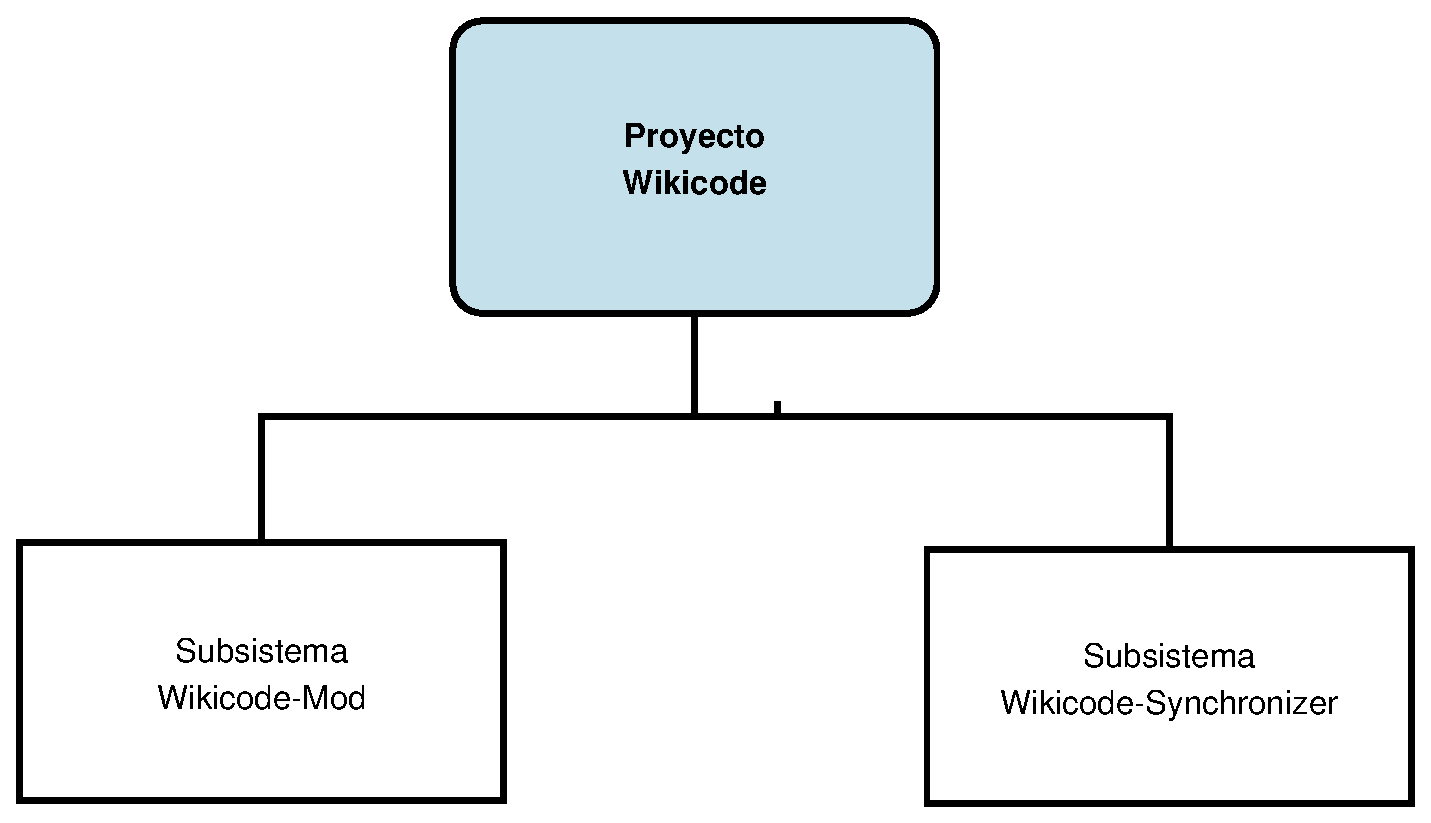
\includegraphics[width=\textwidth]{./img/c3-subsistemas.eps}
	\caption{Gráfico de Subsistemas}
\end{figure}

\subsection{Subsistema Wikicode-Mod}

El subsistema \emph{Wikicode-Mod} es el encargado de interactuar con el usuario y de aceptar o denegar las peticiones que este le pida. Será también el artífice de llevar la información al subsistema encargado de la sincronización del código fuente y de recibir el código actualizado y mostrarlo al usuario final. Dicho de otra manera, el subsistema \emph{Wikicode-Mod} servirá de interfaz entre los usuarios y el entorno de programación embebido en Moodle.

Este subsistema se puede dividir en estos ocho módulos para realizar lo expuesto anteriormente:

\begin{enumerate}
	\item Módulo para configurar el módulo dentro de la plataforma e-learning. A partir de este momento, se le llamará subsistema \emph{Configurar}.
	\item Módulo para visualizar el código fuente en texto plano. A partir de este momento, se le llamará subsistema \emph{Visualización del Código}.
	\item Módulo para editar el código fuente en lenguaje C. A partir de este momento, se le llamará subsistema \emph{Edición del Código}.
	\item Módulo para que los usuarios puedan interactuar de modo síncrono. A partir de este momento, se le llamará subsistema \emph{Chat}.
	\item Módulo para compilar el código fuente desarrollado en el proyecto. A partir de este momento, se le llamará subsistema \emph{Compilación del Código}.
	\item Módulo para visualizar las versiones antiguas del código fuente. A partir de este momento, se le llamará subsistema \emph{Histórico de Código}.
	\item Módulo para visualizar las estadísticas del código fuente. A partir de este momento, se le llamará subsistema \emph{Log Proyecto}.
	\item Módulo para administrar el proyecto. A partir de este momento, se le llamará subsistema \emph{Administración}.
\end{enumerate}

\begin{figure}[h]
	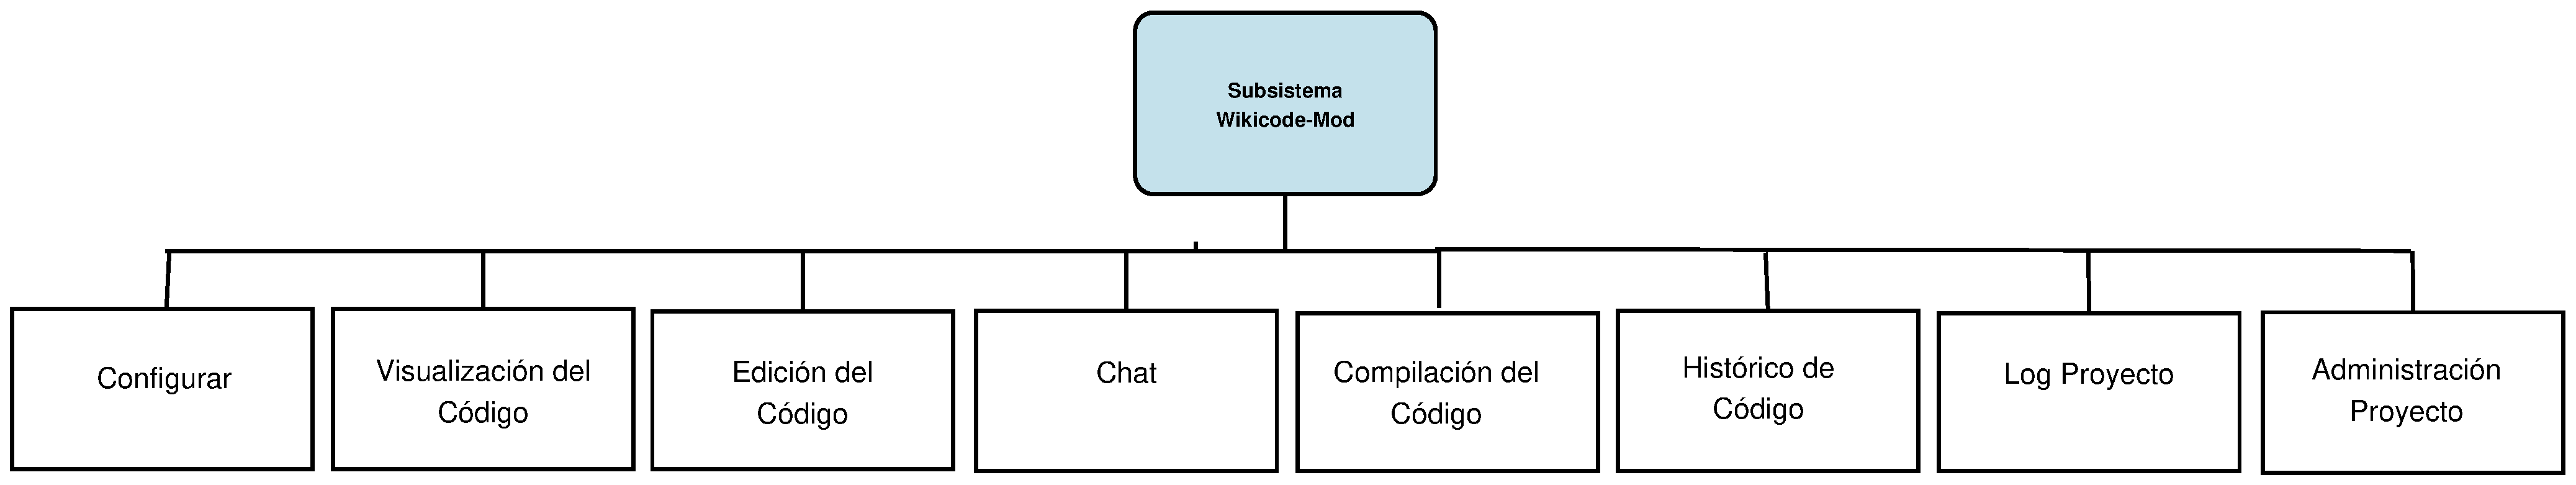
\includegraphics[width=\textwidth]{./img/c3-sub-mod.eps}
	\caption{Gráfico de Subsistema Wikicode-Mod}
\end{figure}

A continuación se van a describir la principales funcionalidades y requisitos para cada subsistema:

\subsubsection{Configurar}

Módulo encargado de crear y parametrizar de los proyectos Wikicode embebidos en Moodle. 

Los requisitos del módulo \emph{Configurar} son:

\begin{itemize}
	\item \textbf{RC1:} Se debe indicar la ruta del compilador o compiladores con los que se quiere crear la aplicación.
	\item \textbf{RC2:} Se debe posibilitar al tutor de personalizar si quiere que el código se edite de modo individual o grupal.
	\item \textbf{RC3:} Se debe permitir la parametrización de otros campos informativos como Nombre, Descripción, etc.
\end{itemize}

\subsubsection{Visualización del Código}

Módulo encargado de mostrar al usuario el código fuente desarrollado en texto plano.

Los requisitos del módulo \emph{Visualización del Código} son:

\begin{itemize}
	\item \textbf{RVC1:} Se debe mostrar el código fuente desarrollado sin ninguna etiqueta.
	\item \textbf{RVC2:} Se debe permitir al tutor la posibilidad de elección de grupo en caso de que el módulo se haya desarrollado de modo grupal.
\end{itemize}
	
\subsubsection{Edición del Código}

Módulo encargado de permitir la escritura al usuario de código fuente y a su vez de impedir acciones no permitidas. También debe de informar de una serie de requisitos que se marcaban como objetivos.

Los requisitos del módulo \emph{Edición del Código} son:

\begin{itemize}
	\item \textbf{REC1:} Permitir al usuario el desarrollo de código fuente en lenguaje C.
	\item \textbf{REC2:} Se debe proporcionar al usuario información para ayudarlo en la escritura del código fuente, mostrando la línea de código sobre la que nos encontramos actualmente.
	\item \textbf{REC3:} Se ha de parsear el código, ayudándose de colores y estilos tipográficos, para informar al usuario final de palabras claves, cadenas, definiciones, comentarios y funciones.
	\item \textbf{REC4:} Se debe impedir al usuario editar una parte bloqueada por otro usuario. 
	\item \textbf{REC5:} Se debe de informar al usuario sobre qué partes están bloqueadas y qué usuario la tiene bloqueada.
	\item \textbf{REC6:} Se debe de bloquear automáticamente la función que el usuario está modificando para impedir que otros usuarios puedan cambiarla.
\end{itemize}
	
\subsubsection{Chat}

Módulo encargado de permitir la interlocución entre los distintos usuarios de un proyecto Wikicode.

Los requisitos del módulo \emph{Chat} son:

\begin{itemize}
	\item \textbf{RCH1:} Se debe permitir enviar mensajes y recibirlos de forma grupal y mostrarlos en el interfaz del proyecto.
	\item \textbf{RCH2:} Se deben de conservar los mensajes enviados por todos los usuarios para poder mostrarse de modo posterior.
	\item \textbf{RCH3:} Se debe de mostrar además del mensaje el usuario que lo ha enviado y el momento en que fue enviado.
\end{itemize}
	
\subsubsection{Compilación del Código}

Módulo encargado de compilar el código fuente y de mostrarnos los errores en caso de que lo hubiera.

Los requisitos del módulo \emph{Compilación del Código} son:

\begin{itemize}
	\item \textbf{RCC1:} Se debe de enviar al compilador el código fuente conforme a la versión más actualizada del proyecto, teniendo en cuenta las posibles modificaciones de otros usuarios.
	\item \textbf{RCC2:} En caso de que haya errores en la programación del código, se nos debe de informar de en que línea se han producido dichos errores y mostrarnos una ayuda de como debemos solucionarlos.
\end{itemize}
	
\subsubsection{Histórico de Código}

Módulo encargado de informar de la historia del código fuente y de informarnos de los cambios realizados.

Los requisitos del módulo \emph{Histórico de Código} son:

\begin{itemize}
	\item \textbf{RHC1:} Debe mostrar todas las versiones del código desde su creación hasta el actual.
	\item \textbf{RHC2:} Debe permitir al usuario restaurar una versión antigua.
\end{itemize}
	
\subsubsection{Log Proyecto}

Módulo encargado de ofrecer estadísticas que se han ido recopilando durante la creación y modificación del código fuente.

Los requisitos del módulo \emph{Log Proyecto} son:

\begin{itemize}
	\item \textbf{RLP1:} Se debe de informar del tiempo empleado para la realización del código fuente.
	\item \textbf{RLP2:} Se debe de comunicar al usuario los errores compilando que se han producido durante la realización del proyecto.
\end{itemize}
	
\subsubsection{Administración}

Módulo encargado de facilitar al tutor las opciones necesarias para administrar el proyecto Wikicode.

Los requisitos del módulo \emph{Administración} son:

\begin{itemize}
	\item \textbf{RA1:} No se debe permitir el acceso a usuarios sin el rol de profesor o administrador.
	\item \textbf{RA2:} Permitir al tutor/administrador modificar las opciones creadas durante la configuración y, del mismo modo, eliminar información que no desee almacenar.
\end{itemize}
	
\subsection{Subsistema Wikicode-Synchronizer}

El subsistema \emph{Wikicode-Synchronizer} es el encargado de interactuar con la base de datos y crear los tags oportunos en el código para permitir los bloqueos y desbloqueos necesarios en el código fuente. Dicho de otro modo, es el encargado de hacer de interfaz entre el módulo de Moodle y los datos, modificándolos de manera abstracta al usuario final.

Debido a la naturaleza de los datos, se ha considerado oportuno el dividir este subsistema en los siguiente módulos.

\begin{enumerate}
	\item Módulo que realiza la interacción con la base de datos para salvar/cargar el código. A partir de este momento, se le llamará subsistema \emph{Salvar código}.
	\item Módulo para bloquear y desbloquear funciones dentro del código. A partir de este momento, se le llamará subsistema \emph{Locker/Unlocker código}.
	\item Módulo para actualizar las estadísticas referentes al código que se está tratando. A partir de este momento, se le llamará subsistema \emph{Actualizar Log}.
\end{enumerate}

\begin{figure}[h]
	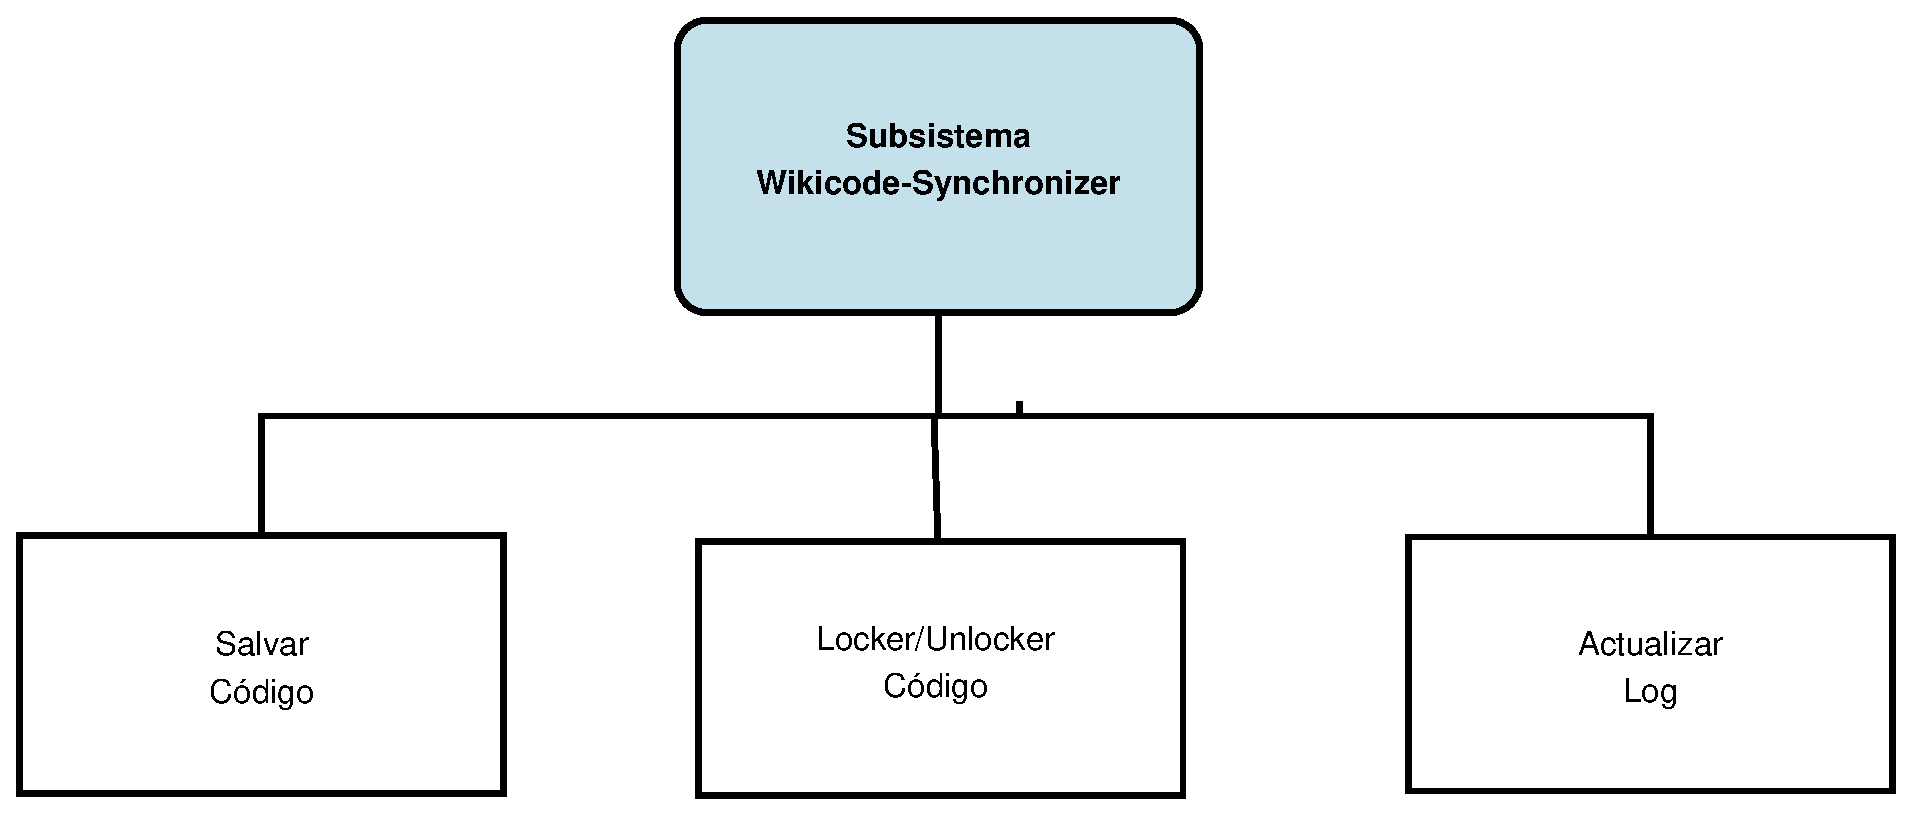
\includegraphics[width=\textwidth]{./img/c3-sub-syn.eps}
	\caption{Gráfico de Subsistema Wikicode-Synchronizer}
\end{figure}

A continuación se van a describir la principales funcionalidades y requisitos para cada subsistema:

\subsubsection{Salvar código}

Módulo encargado de hacer de interfaz entre la base de datos y el proyecto Wikicode. 

Los requisitos del módulo \emph{Salvar código} son:

\begin{itemize}
	\item \textbf{RSC1:} Se debe de obtener el código fuente del editor cada vez que se pulse una tecla clave.
	\item \textbf{RSC2:} Se considerará tecla clave el punto y coma (\textbf{;}), el intro y la apertura de corchetes (\textbf{\{}).
	\item \textbf{RSC3:} Se debe, tras comprobar que la función está bloqueada por el usuario, cambiar la función que ha sido modificada por el usuario en el código fuente global.
	\item \textbf{RSC4:} Se debe, si la función está bloqueada por otro usuario, devolver un código de error y no almacenar nada en base de datos.
	\item \textbf{RSC5:} Se debe, si el código ha sido modificado, enviar al editor el nuevo código fuente modificado. Este código debe tener embebida la información sobre sus bloqueos.
\end{itemize}

\subsubsection{Locker/Unlocker código}

Módulo encargado de recibir el código fuente y bloquear o desbloquear funciones del código.

Los requisitos del módulo \emph{Locker/Unlocker código} son:

\begin{itemize}
	\item \textbf{RLU1:} Se debe de bloquear el código de una función, si el usuario así lo desea, desde el principio de sus comentarios hasta la finalización del último corchete.
	\item \textbf{RLU2:} Si se desea bloquear una función ya bloqueada el sistema debe devolver un mensaje de error.
	\item \textbf{RLU3:} Se debe de permitir a cualquier usuario bloquear una función si esta ha sido desbloqueada.
	\item \textbf{RLU4:} Se debe de permitir a un usuario que tenga una función bloqueada desbloquearla cuando este desee.
\end{itemize}

\subsubsection{Actualizar Log}

Módulo encargado de actualizar la información referente a las estadísticas del código sobre el que se está trabajando.

Los requisitos del módulo \emph{Actualizar Log} son:

\begin{itemize}
	\item \textbf{RAL1:} La duración del proyecto se contabilizará desde el inicio de su escritura hasta la última modificación realizada.
	\item \textbf{RAL2:} Cada vez que exista una compilación errónea se aumentará en uno este dato. Se inicializará a cero.
\end{itemize}

\section{Especificación de la interfaz}

En este apartado se pretende analizar la interfaz de la aplicación a desarrollar. Partiendo de la interfaz utilizada por la plataforma Moodle, se ha intentado mantener la sencillez y claridad de la misma. Realmente, la interfaz de nuestra aplicación consiste en un módulo de Moodle que, como hemos comentado, mantendrá su sencillez, claridad y estilo. Este módulo contiene fundamentalmente una serie de acciones que son las que puede elegir el usuario: Creación, Visualización, Edición, Visualización del Histórico y Visualización de Estadísticas.

De esta manera, las interfaces que se encontrará el usuario al acceder a un curso determinado a través de moodle son:

\begin{itemize}
	\item Estructura general de la interfaz del curso. Esta estructura vendrá presentada en la siguiente figura:
\end{itemize}

\begin{figure}[h]
	\centering
	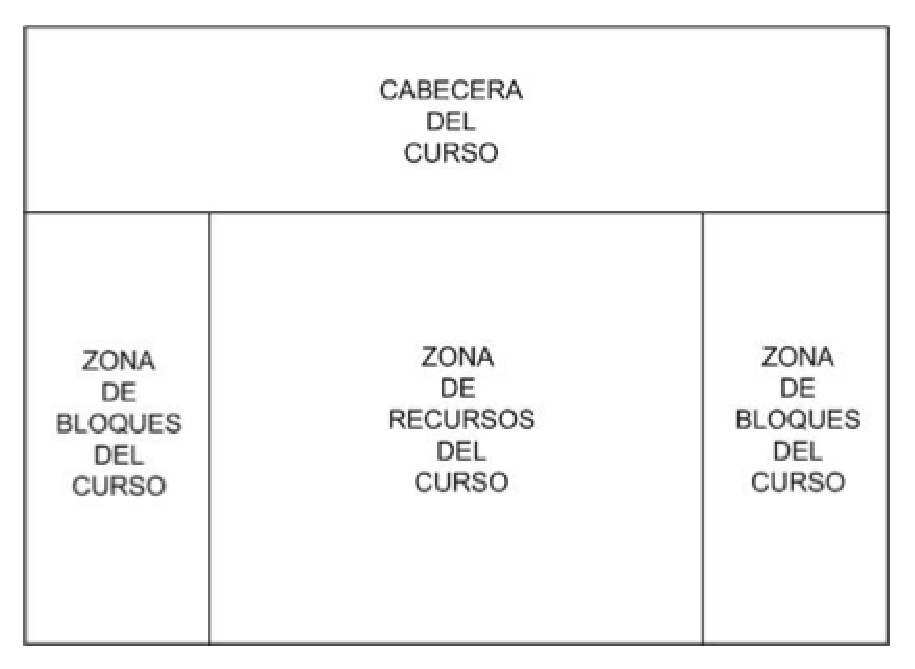
\includegraphics[width=0.5\textwidth]{./img/c3-estructuracursomoodle.eps}
	\caption{Estructura general de la interfaz del curso}
\end{figure}

Cuando un usuario desee acceder a la aplicación desarrollada o un tutor desee tanto entrar como crear un nuevo código fuente para que lo editen los usuarios lo hará desde la zona de recursos del curso.

\begin{itemize}
	\item Estructura general de creación de un nuevo módulo Wikicode. Esta estructura vendrá presentada en la siguiente figura:
\end{itemize}

\begin{figure}[h]
	\centering
	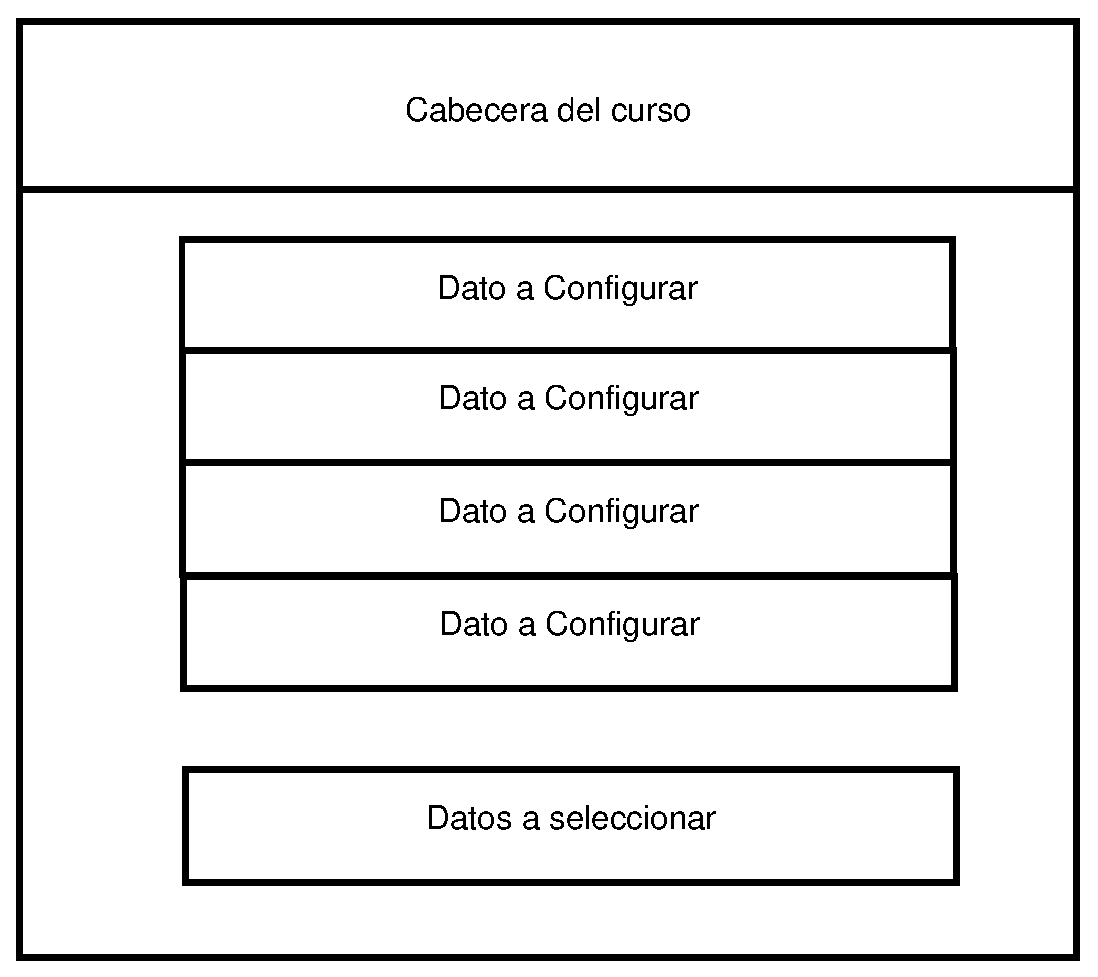
\includegraphics[width=0.5\textwidth]{./img/c3-create.eps}
	\caption{Estructura de la interfaz de creación}
\end{figure}

En este esquema podemos observar que se presenta un formulario a rellenar con los datos necesarios para la creación de un nuevo módulo Wikicode. Una vez queden introducidos o seleccionados, habrá que confirmar los cambios para que queden registrados en el sistema.

\newpage

\begin{itemize}
	\item Estructura general de visualización del código fuente en un módulo Wikicode. Esta estructura vendrá presentada en la siguiente figura:
\end{itemize}

\begin{figure}[h]
	\centering
	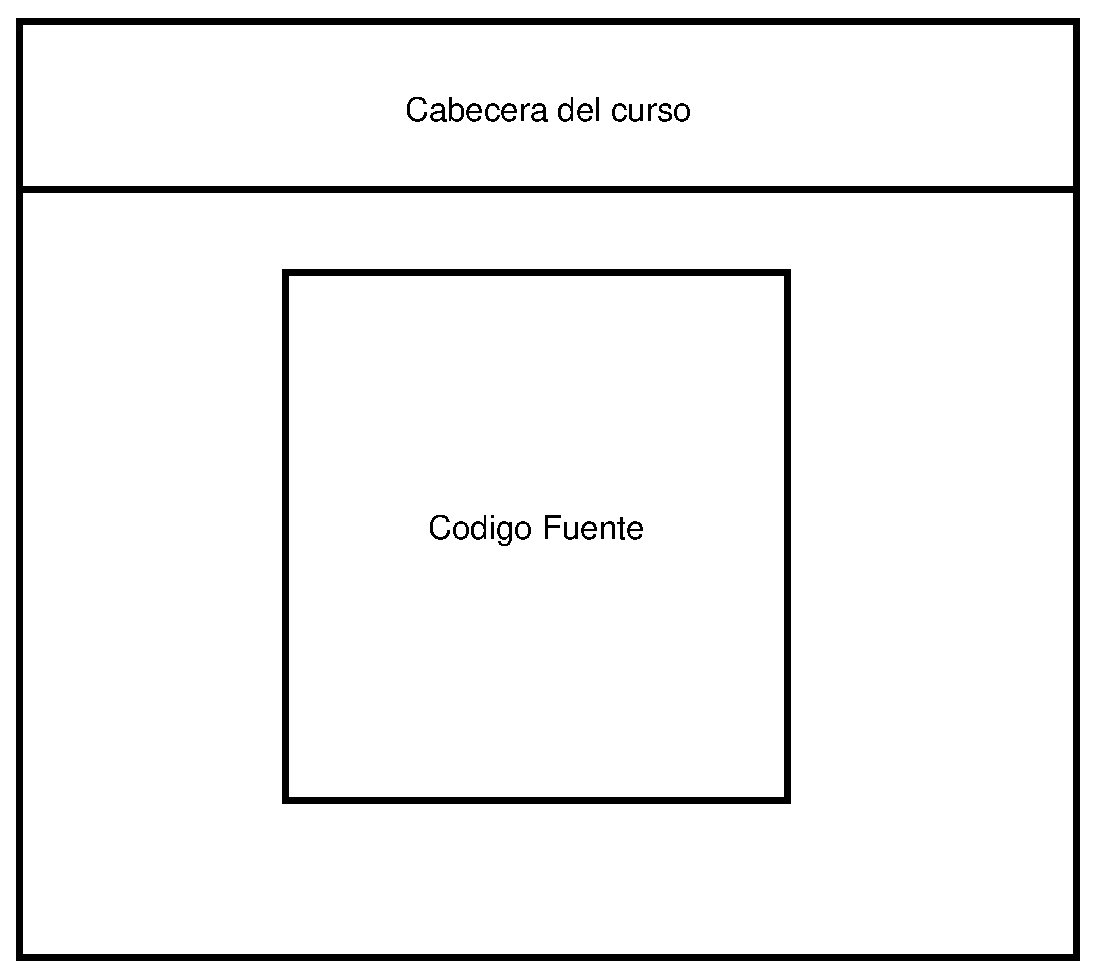
\includegraphics[width=0.5\textwidth]{./img/c3-view.eps}
	\caption{Estructura de la interfaz de vista}
\end{figure}

En este esquema podemos observar que se mantiene la cabecera del curso, en el que tendremos un menú superior para navegar por las opciones de la Wikicode, y un cuadro de texto con el código fuente que ha sido desarrollado.

\begin{itemize}
	\item Estructura general de edición del código fuente en un módulo Wikicode. Esta estructura vendrá presentada en la siguiente figura:
\end{itemize}

\begin{figure}[h]
	\centering
	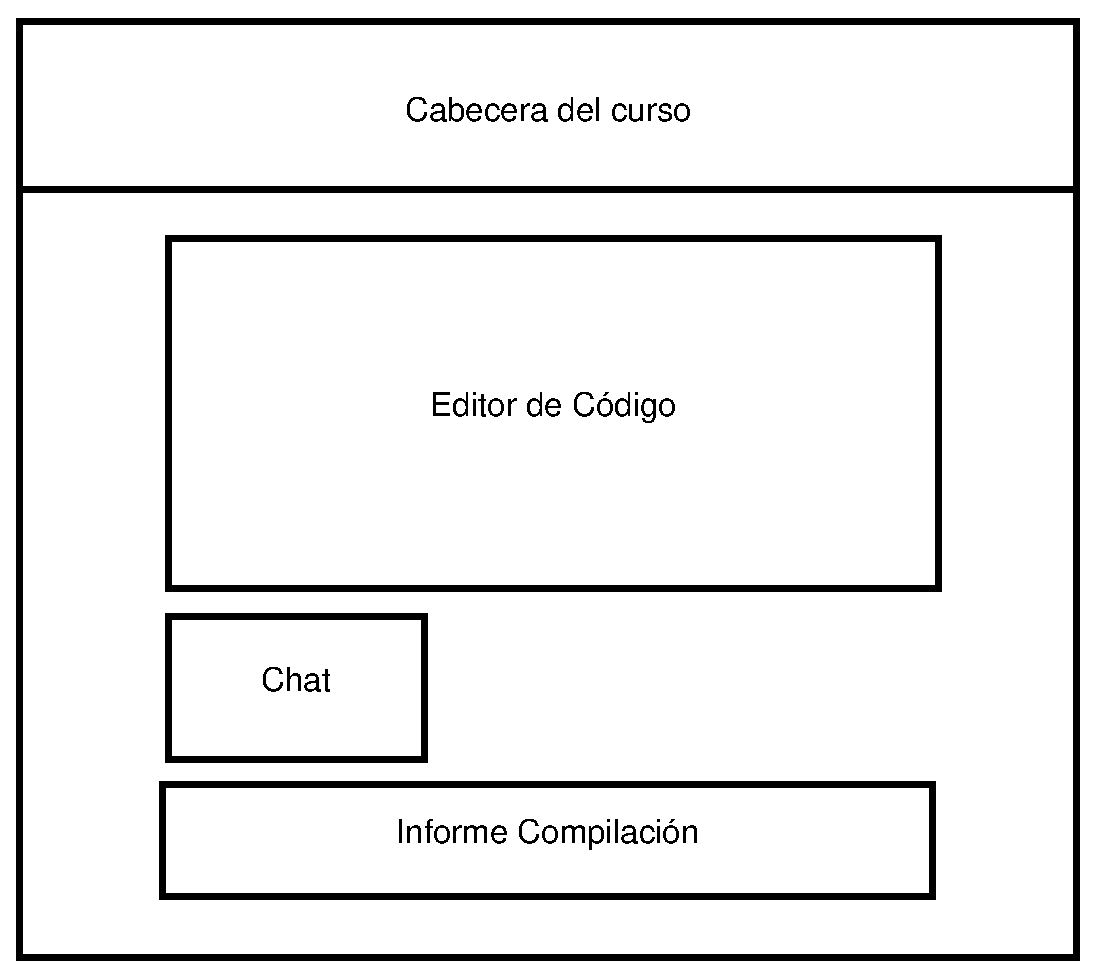
\includegraphics[width=0.5\textwidth]{./img/c3-edit.eps}
	\caption{Estructura de la interfaz de edición del código fuente}
\end{figure}

En esta estructura, vemos como en la parte superior conservamos la cabecera del curso para poder navegar por sus opciones. En el resto del cuerpo tenemos un editor de código para que el usuario pueda escribir el programa, un chat para comunicarse de modo síncrono con el resto de usuarios e información sobre los posibles errores de compilación.

\begin{itemize}
	\item Estructura general del histórico en un módulo Wikicode. Esta estructura vendrá presentada en la siguiente figura:
\end{itemize}

\begin{figure}[h]
	\centering
	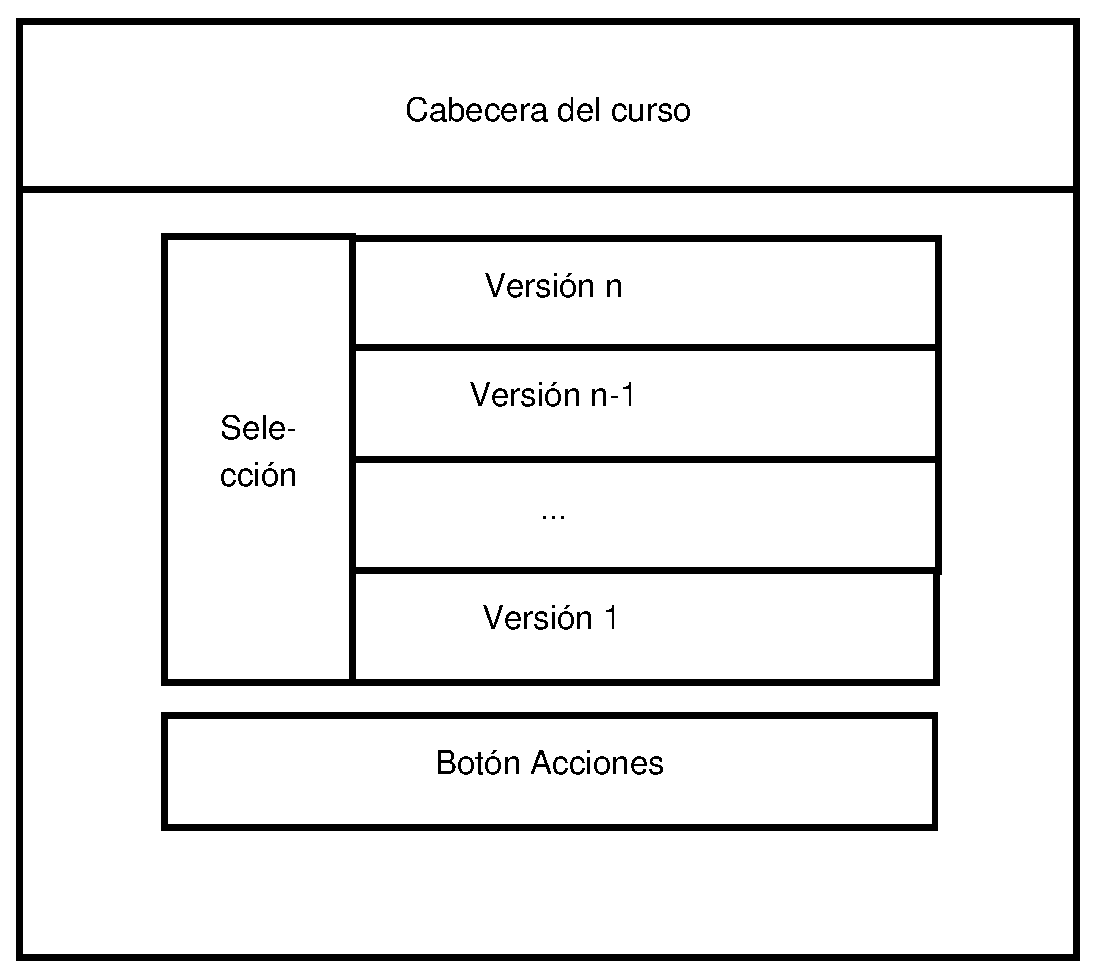
\includegraphics[width=0.5\textwidth]{./img/c3-history.eps}
	\caption{Estructura de la interfaz del histórico de un código fuente}
\end{figure}

Al igual que con las anteriores interfaces en esta seguimos manteniendo la misma estructura, un menú superior con información sobre el curso y la posibilidad de navegar más rápidamente. En el cuerpo se mostrarán todas las versiones desarrolladas por los usuarios, un \emph{radiobutton} para posibilitar elegir alguna en concreto y una botonera para poder realizar acciones sobre ellas.

\begin{itemize}
	\item Estructura general de visualización de las estadísticas de un módulo Wikicode. Esta estructura vendrá presentada en la siguiente figura:
\end{itemize}

\begin{figure}[h]
	\centering
	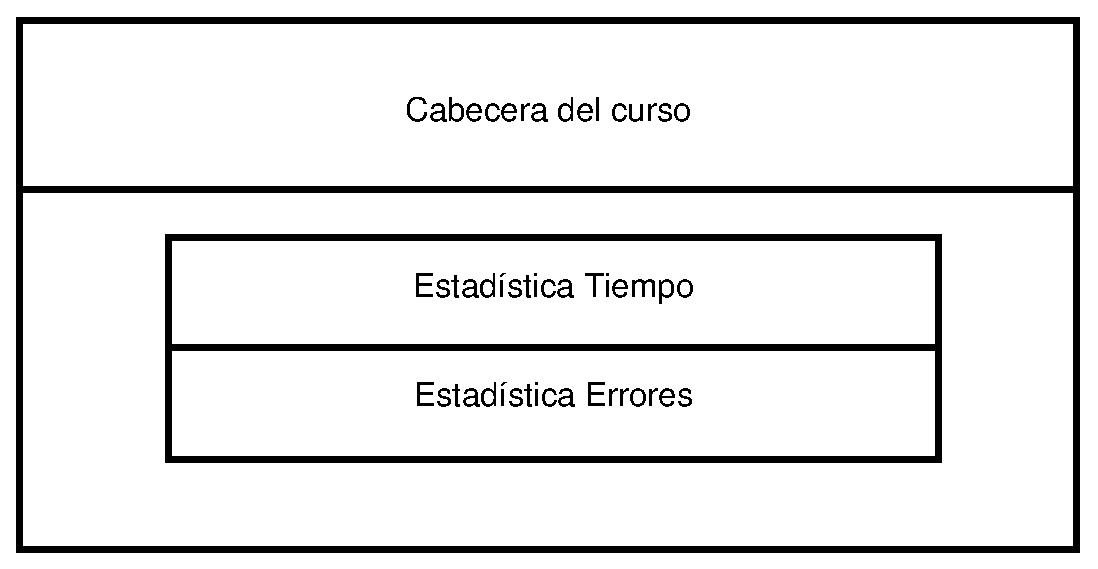
\includegraphics[width=0.5\textwidth]{./img/c3-logs.eps}
	\caption{Estructura de la interfaz de la información estadística de una Wikicode}
\end{figure}

De nuevo mantenemos la cabecera en la parte superior del interfaz, con las ventajas que ya hemos comentado con anterioridad de navegación, y en el cuerpo de esta mostraremos los resultados respecto a las estadísticas calculadas. De esta manera en primer lugar se presentará el tiempo necesitado y a continuación se informará del número de errores producidos. 

\section{Modelo funcional}

Para explicar el modelo funcional utilizado vamos a aplicar casos de uso. Un caso de uso se define como una colección de escenarios con éxitos y fallo relacionados, que describe a los actores utilizando un sistema para satisfacer un objetivo. 

Como hemos comentado anteriormente, el proyecto se ha divido en dos subsistemas que pueden ser estudiados por separado: Wkicode-Mod \emph{Módulo de Moodle} y Wikicode-Synchronizer \emph{Tratamiento de datos}. Por tanto, especificaremos los casos de uso así como los actores que están involucrados para cada uno de los sistemas.

\subsection{Identificación de actores}

Antes de nada tendremos que identificar los actores que interactuarán con nuestros sistemas. De esta manera, contaremos con los siguientes actores:

\subsubsection{Tutor}

A continuación se especifican las características que debe tener el actor \emph{Tutor}:

\begin{table}[h]
\centering
\begin{tabular}{ | p{0.25\textwidth} | p{0.60\textwidth} | }
	\hline
	\multicolumn{2}{|c|}{ACTOR: Tutor} \\
	\hline
	Identificador  & Tutor \\
	\hline 
	Id-Padre & No tiene \\
	\hline
	Descripción & Persona encargada de crear la Wikicode y de configurar los parámetros necesarios. Está involucrada con el sistema Wikicode-Mod.\\
	\hline
\end{tabular}
\caption{Descripción del Tutor}
\end{table}

\subsubsection{Usuario}

A continuación se especifican las características que debe tener el actor \emph{Usuario}:

\begin{table}[h]
\centering
\begin{tabular}{ | p{0.25\textwidth} | p{0.60\textwidth} | }
	\hline
	\multicolumn{2}{|c|}{ACTOR: Usuario} \\
	\hline
	Identificador  & Usuario \\
	\hline 
	Id-Padre & No tiene \\
	\hline
	Descripción & Persona encargada de editar el código fuente, comunicarse vía chat con otros usuarios y llamar al compilador de Código fuente. También tiene la posibilidad de navegar por el histórico del código y visualizar las estadísticas de la Wikicode. Está involucrada con el sistema Wikicode-Mod.\\
	\hline
\end{tabular}
\caption{Descripción del Tutor}
\end{table}

\newpage

\subsubsection{Módulo Wikicode-Mod}

A continuación se especifican las características que debe tener el actor \emph{Módulo Wikicode-Mod}:

\begin{table}[h]
\centering
\begin{tabular}{ | p{0.25\textwidth} | p{0.60\textwidth} | }
	\hline
	\multicolumn{2}{|c|}{ACTOR: Módulo Wikicode-Mod} \\
	\hline
	Identificador  & Módulo Wkicode-Mod \\
	\hline 
	Id-Padre & No tiene \\
	\hline
	Descripción & Módulo encargado de recibir las peticiones del usuario, así como la configuración para la creación del mismo. Es el encargado de llamar al compilador y de mostrarnos el mensaje de este. A su vez es el que se ocupa de escribir y leer los ficheros referentes al chat. También se encargará de hacer las peticiones necesarias al subsistema encargado de sincronizar y almacenar el código, así como de leer y mostrar el código fuente una vez haya sido devuelto. Está involucrada con el sistema Wikicode-Synchronizer.\\
	\hline
\end{tabular}
\caption{Descripción del Módulo Wikicode-Mod}
\end{table}

\subsubsection{Módulo Wikicode-Synchronizer}

A continuación se especifican las características que debe tener el actor \emph{Módulo Wikicode-Synchronizer}:

\begin{table}[h]
\centering
\begin{tabular}{ | p{0.25\textwidth} | p{0.60\textwidth} | }
	\hline
	\multicolumn{2}{|c|}{ACTOR: Módulo Wikicode-Synchronizer} \\
	\hline
	Identificador  & Módulo Wikicode-Synchronizer \\
	\hline 
	Id-Padre & No tiene \\
	\hline
	Descripción & Módulo encargado de hacer las modificaciones necesarias en el código fuente, así como desbloquear y bloquear para un usuario específico partes de este. Es el encargado de actualizar las estadísticas relacionadas con la Wikicode que se está trabajando. También debe de enviar al subsistema encargado de mostrar el código éste una vez actualizado. Está involucrada con el sistema Wikicode-Mod.\\
	\hline
\end{tabular}
\caption{Descripción del Módulo Wikicode-Synchronizer}
\end{table}

\subsection{Casos de uso de trazo grueso}

El siguiente paso para describir el modelo funcional es identificar los principales casos de uso.

Para el sistema Wikicode éstos serán los siguientes:

\begin{itemize}
	\item C1. Caso de uso Creación y Parametrización de la actividad Wikicode. Cuando el \emph{Tutor} seleccione en la pantalla principal del curso que desea crear una nueva Wikicode para los usuarios del curso deberá configurar una serie de opciones. Una vez creada, el \emph{Tutor} también podrá administrar dichas opciones.
	\item C2. Caso de uso Visualización del código desarrollado. Tanto el \emph{Tutor} como el \emph{Alumno} pueden acceder a visualizar una Wikicode sin necesidad de querer realizar una acción sobre ella.
	\item C3. Caso de uso Edición del Código. Una vez esté creada una Wikicode, lo primero que hay que hacer es insertar contenido en ella, la cual se hace desde un editor web embebido dentro de la propia plataforma e-learning. El \emph{Alumno} o grupo de estos podrá desarrollar libremente el código fuente. Durante la edición se actualizarán estadísticas.
	\item C4. Caso de uso Bloqueo del Código. Una vez que el \emph{Alumno} empieza a editar un código fuente, automáticamente se bloquea la función que está modificando o creando para que otros usuarios no puedan acceder a ella.
	\item C5. Caso de uso Desbloqueo del Código. Una vez que el \emph{Alumno} ha terminado una función dentro de un código fuente, debe acudir a la opción que tiene en su interfaz de desbloquear funciones y marcar cual quiere desbloquear para que otro \emph{Alumno} pueda modificarla.
	\item C6. Caso de uso Salvar Código. Cada vez que un \emph{Alumno} pulse una tecla clave en el editor, este realizará una petición al subsistema encargado de sincronizar su información y esta se almacenará en base de datos.
	\item C7. Caso de uso Interacción mediante Chat con otros usuarios. Un \emph{Alumno} puede tener la necesidad de comunicarse con otros miembros del grupo que estén colaborando para modificar una Wikicode, y puede hacerlo a través de esta herramienta que de tipo chat que llegará como mensaje de aviso al resto usuarios.
	\item C8. Caso de uso Compilación de código fuente. Un \emph{Alumno} que así lo desee puede llamar a un compilador y este, a través del interfaz diseñado para la edición de código fuente, mostrar los resultados de la compilación de su código. Si la compilación es correcta puede descargar el ejecutable si así lo desea.
	\item C9. Caso de uso Consulta de histórico y restauración de versiones. Tanto un \emph{Alumno} como un \emph{Tutor} pueden acceder al histórico de una Wikicode para consultar el código en otras fechas. Una vez dentro de una versión antigua comprobarán el código y lo restaurarán si así se desea.
	\item C10. Caso de uso Consulta de Estadísticas. Un \emph{Alumno}, así como un \emph{Tutor}, pueden comprobar la información estadística de una Wikicode si así lo desean. En ella pueden ver la duración de edición de código y el número de compilaciones erróneas.
\end{itemize}

\subsubsection{Casos de uso para el sistema Wikicode}

\textbf{CASO DE USO C1: Creación y Parametrización de la actividad Wikicode.} Este es el diagrama correspondiente al caso de uso C1:

\begin{table}[h]
\centering
\begin{tabular}{ | p{0.30\textwidth} | p{0.60\textwidth} | }
	\hline
	\multicolumn{2}{|c|}{CASO DE USO C1: Creación y Parametrización de la actividad Wikicode} \\
	\hline
	Identificador  & C1 \\
	\hline 
	Id-Padre & No tiene \\
	\hline
	Id-Requisito de Soporte & RC1, RC2, RC3, RA1, RA2 \\
	\hline
	Descripción & Se describe el proceso de creación y parametrización de la actividad Wikicode. \\
	\hline
\end{tabular}
\caption{Caso de Uso C1: Creación y Parametrización de la actividad Wikicode}
\end{table}

\vspace{2cm}

\textbf{CASO DE USO C2: Visualización del código desarrollado.} Este es el diagrama correspondiente al caso de uso C2:

\begin{table}[h]
\centering
\begin{tabular}{ | p{0.3\textwidth} | p{0.60\textwidth} | }
	\hline
	\multicolumn{2}{|c|}{CASO DE USO C2: Visualización del código desarrollado} \\
	\hline
	Identificador  & C2 \\
	\hline 
	Id-Padre & No tiene \\
	\hline
	Id-Requisito de Soporte & RVC1, RVC2 \\
	\hline
	Descripción & Se describe el proceso de visualización del código desarrollado. \\
	\hline
\end{tabular}
\caption{Caso de Uso C2: Visualización del código desarrollado}
\end{table}

\newpage

\textbf{CASO DE USO C3: Edición del código desarrollado.} Este es el diagrama correspondiente al caso de uso C3:

\begin{table}[h]
\centering
\begin{tabular}{ | p{0.3\textwidth} | p{0.60\textwidth} | }
	\hline
	\multicolumn{2}{|c|}{CASO DE USO C3: Edición del Código} \\
	\hline
	Identificador  & C3 \\
	\hline 
	Id-Padre & No tiene \\
	\hline
	Id-Requisito de Soporte & REC1, REC2, REC3, REC4, REC5, RAL1 \\
	\hline
	Descripción & Se describe el proceso de edición del código fuente. \\
	\hline
\end{tabular}
\caption{Caso de Uso C3: Edición del Código}
\end{table}

\vspace{2cm}

\textbf{CASO DE USO C4: Bloqueo del Código.} Este es el diagrama correspondiente al caso de uso C4:

\begin{table}[h]
\centering
\begin{tabular}{ | p{0.3\textwidth} | p{0.60\textwidth} | }
	\hline
	\multicolumn{2}{|c|}{CASO DE USO C4: Bloqueo del Código} \\
	\hline
	Identificador  & C4 \\
	\hline 
	Id-Padre & No tiene \\
	\hline
	Id-Requisito de Soporte & REC6, RLU1, RLU2, RLU3 \\
	\hline
	Descripción & Se describe el proceso de bloqueo del código fuente. \\
	\hline
\end{tabular}
\caption{Caso de Uso C4: Bloqueo del Código}
\end{table}

\vspace{2cm}

\textbf{CASO DE USO C5: Desbloqueo del Código.} Este es el diagrama correspondiente al caso de uso C5:

\begin{table}[h]
\centering
\begin{tabular}{ | p{0.3\textwidth} | p{0.60\textwidth} | }
	\hline
	\multicolumn{2}{|c|}{CASO DE USO C5: Desbloqueo del Código} \\
	\hline
	Identificador  & C5 \\
	\hline 
	Id-Padre & No tiene \\
	\hline
	Id-Requisito de Soporte & RLU4 \\
	\hline
	Descripción & Se describe el proceso de desbloqueo del código fuente. \\
	\hline
\end{tabular}
\caption{Caso de Uso C5: Desbloqueo del Código}
\end{table}

\newpage

\textbf{CASO DE USO C6: Salvar Código.} Este es el diagrama correspondiente al caso de uso C6:

\begin{table}[h]
\centering
\begin{tabular}{ | p{0.3\textwidth} | p{0.60\textwidth} | }
	\hline
	\multicolumn{2}{|c|}{CASO DE USO C6: Salvar Código} \\
	\hline
	Identificador  & C6 \\
	\hline 
	Id-Padre & No tiene \\
	\hline
	Id-Requisito de Soporte & RSC1, RSC2, RSC3, RSC4, RSC5 \\
	\hline
	Descripción & Se describe el proceso de salvar el código fuente. \\
	\hline
\end{tabular}
\caption{Caso de Uso C6: Salvar Código}
\end{table}

\vspace{2cm}

\textbf{CASO DE USO C7: Interacción mediante Chat con otros usuarios.} Este es el diagrama correspondiente al caso de uso C7:

\begin{table}[h]
\centering
\begin{tabular}{ | p{0.3\textwidth} | p{0.60\textwidth} | }
	\hline
	\multicolumn{2}{|c|}{CASO DE USO C7: Interacción mediante Chat con otros usuarios} \\
	\hline
	Identificador  & C7 \\
	\hline 
	Id-Padre & No tiene \\
	\hline
	Id-Requisito de Soporte & RCH1, RCH2, RCH3 \\
	\hline
	Descripción & Se describe el proceso de interacción mediante chat con otros usuarios. \\
	\hline
\end{tabular}
\caption{Caso de Uso C7: Interacción mediante Chat con otros usuarios}
\end{table}

\vspace{2cm}

\textbf{CASO DE USO C8: Compilación de código fuente.} Este es el diagrama correspondiente al caso de uso C8:

\begin{table}[h]
\centering
\begin{tabular}{ | p{0.3\textwidth} | p{0.60\textwidth} | }
	\hline
	\multicolumn{2}{|c|}{CASO DE USO C8: Compilación de código fuente} \\
	\hline
	Identificador  & C8 \\
	\hline 
	Id-Padre & No tiene \\
	\hline
	Id-Requisito de Soporte & RCC1, RCC2, RAL2 \\
	\hline
	Descripción & Se describe el proceso de compilación de código fuente. \\
	\hline
\end{tabular}
\caption{Caso de Uso C8: Compilación de código fuente}
\end{table}

\newpage

\textbf{CASO DE USO C9: Consulta de histórico y restauración de versiones.} Este es el diagrama correspondiente al caso de uso C9:

\begin{table}[h]
\centering
\begin{tabular}{ | p{0.3\textwidth} | p{0.60\textwidth} | }
	\hline
	\multicolumn{2}{|c|}{CASO DE USO C9: Consulta de histórico y restauración de versiones} \\
	\hline
	Identificador  & C9 \\
	\hline 
	Id-Padre & No tiene \\
	\hline
	Id-Requisito de Soporte & RHC1, RHC2 \\
	\hline
	Descripción & Se describe el proceso de consulta de histórico y restauración de versiones. \\
	\hline
\end{tabular}
\caption{Caso de Uso C9: Consulta de histórico y restauración de versiones}
\end{table}

\vspace{2cm}

\textbf{CASO DE USO C10: Consulta de Estadísticas.} Este es el diagrama correspondiente al caso de uso C10:

\begin{table}[h]
\centering
\begin{tabular}{ | p{0.3\textwidth} | p{0.60\textwidth} | }
	\hline
	\multicolumn{2}{|c|}{CASO DE USO C10: Consulta de Estadísticas} \\
	\hline
	Identificador  & C10 \\
	\hline 
	Id-Padre & No tiene \\
	\hline
	Id-Requisito de Soporte & RLP1, RLP2 \\
	\hline
	Descripción & Se describe el proceso de consulta de Estadísticas. \\
	\hline
\end{tabular}
\caption{Caso de Uso C10: Consulta de Estadísticas}
\end{table}

\newpage

\subsection{Diagramas de caso de uso}

\subsubsection{Diagramas para el sistema Wikicode}

\begin{itemize}
	\item Diagrama inicial del sistema Wikicode:
\end{itemize}

\begin{figure}[h]
	\centering
	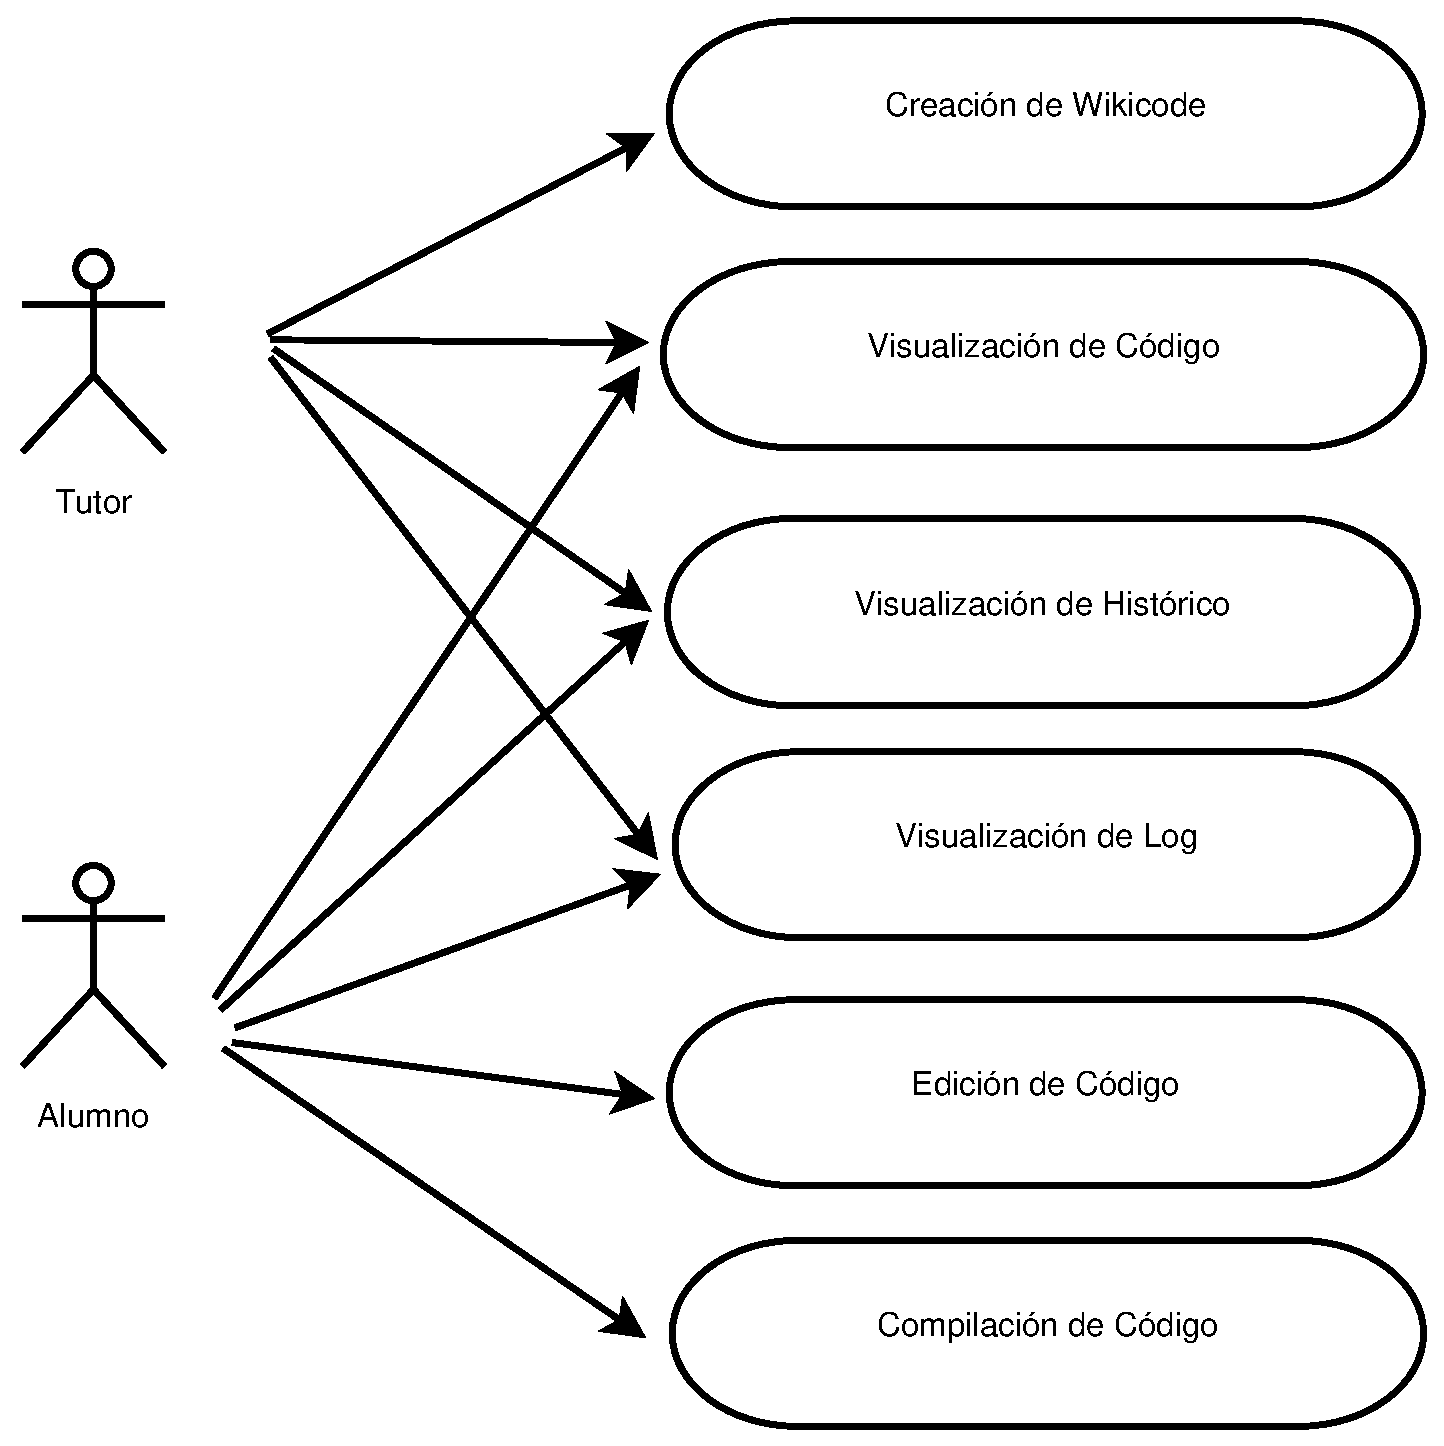
\includegraphics[width=0.5\textwidth]{./img/c3-cu-ini.eps}
	\caption{Diagrama inicial para el sistema Wikicode}
\end{figure}

\vspace{1cm}

\begin{itemize}
	\item Diagrama del Caso de uso C1:
\end{itemize}

\begin{figure}[h]
	\centering
	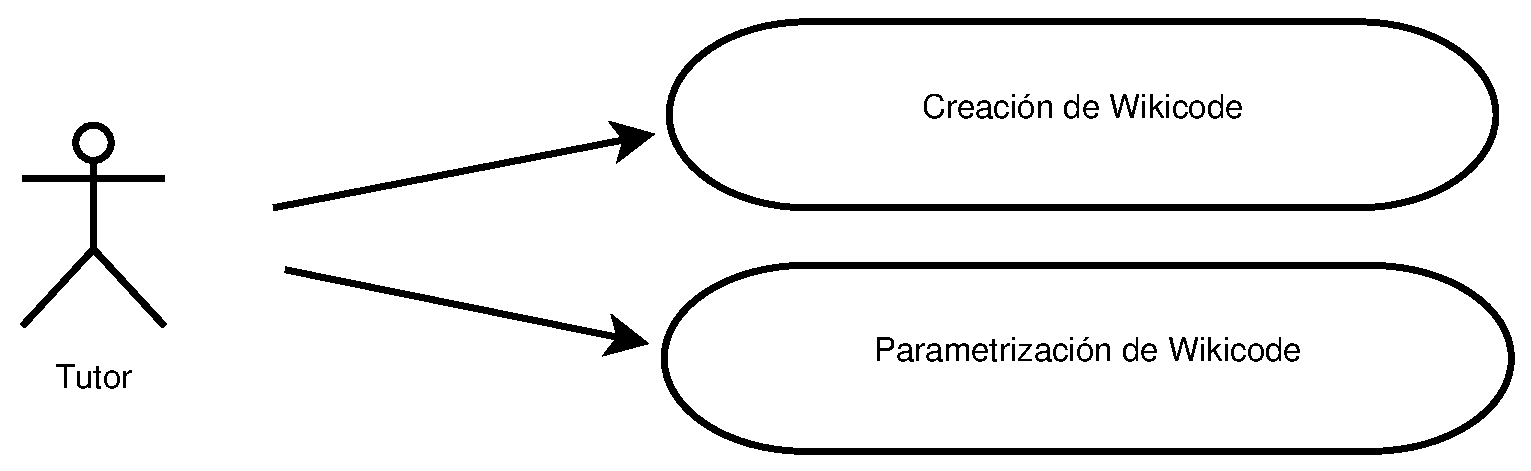
\includegraphics[width=0.5\textwidth]{./img/c3-cu1.eps}
	\caption{Diagrama Caso de uso C1}
\end{figure}

\newpage

\begin{itemize}
	\item Diagrama del Caso de uso C2:
\end{itemize}

\begin{figure}[h]
	\centering
	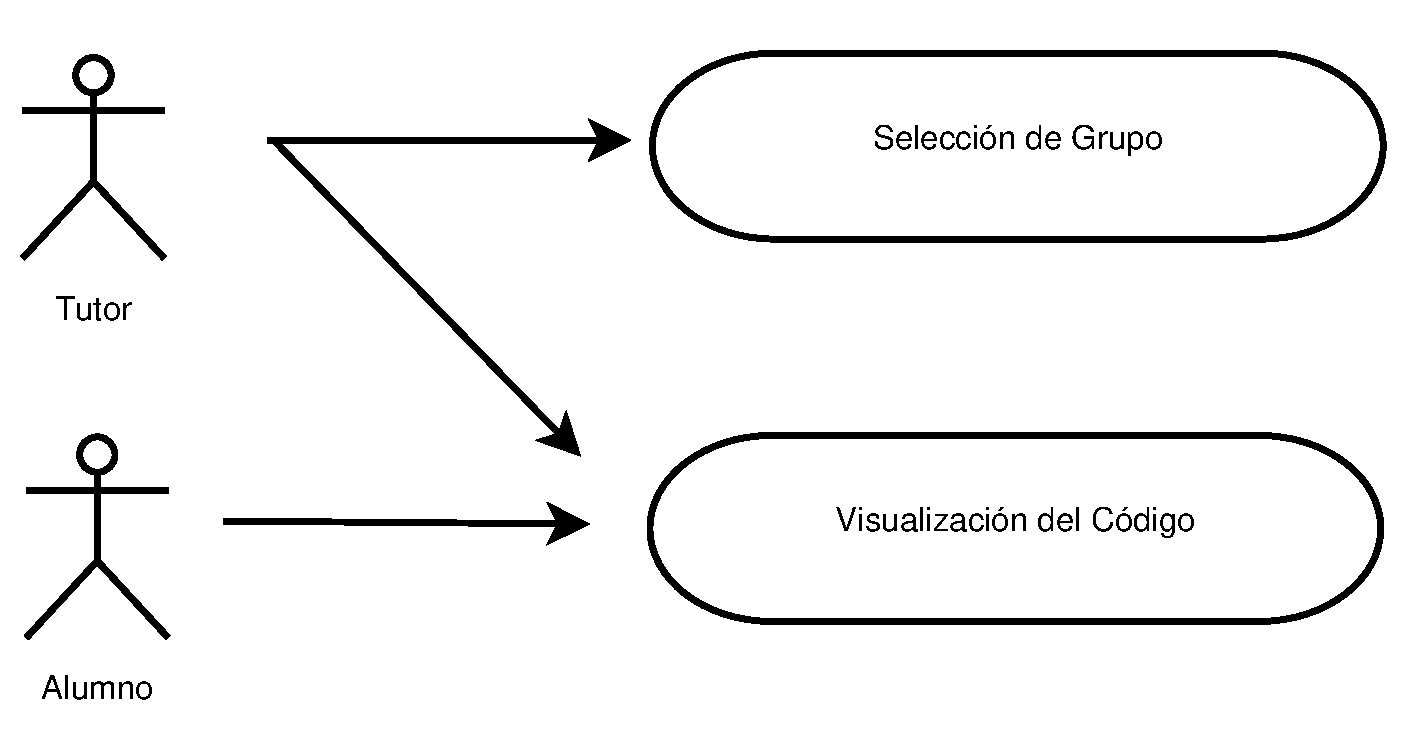
\includegraphics[width=0.5\textwidth]{./img/c3-cu2.eps}
	\caption{Diagrama Caso de uso C2}
\end{figure}

\begin{itemize}
	\item Diagrama del Caso de uso C3:
\end{itemize}

\begin{figure}[h]
	\centering
	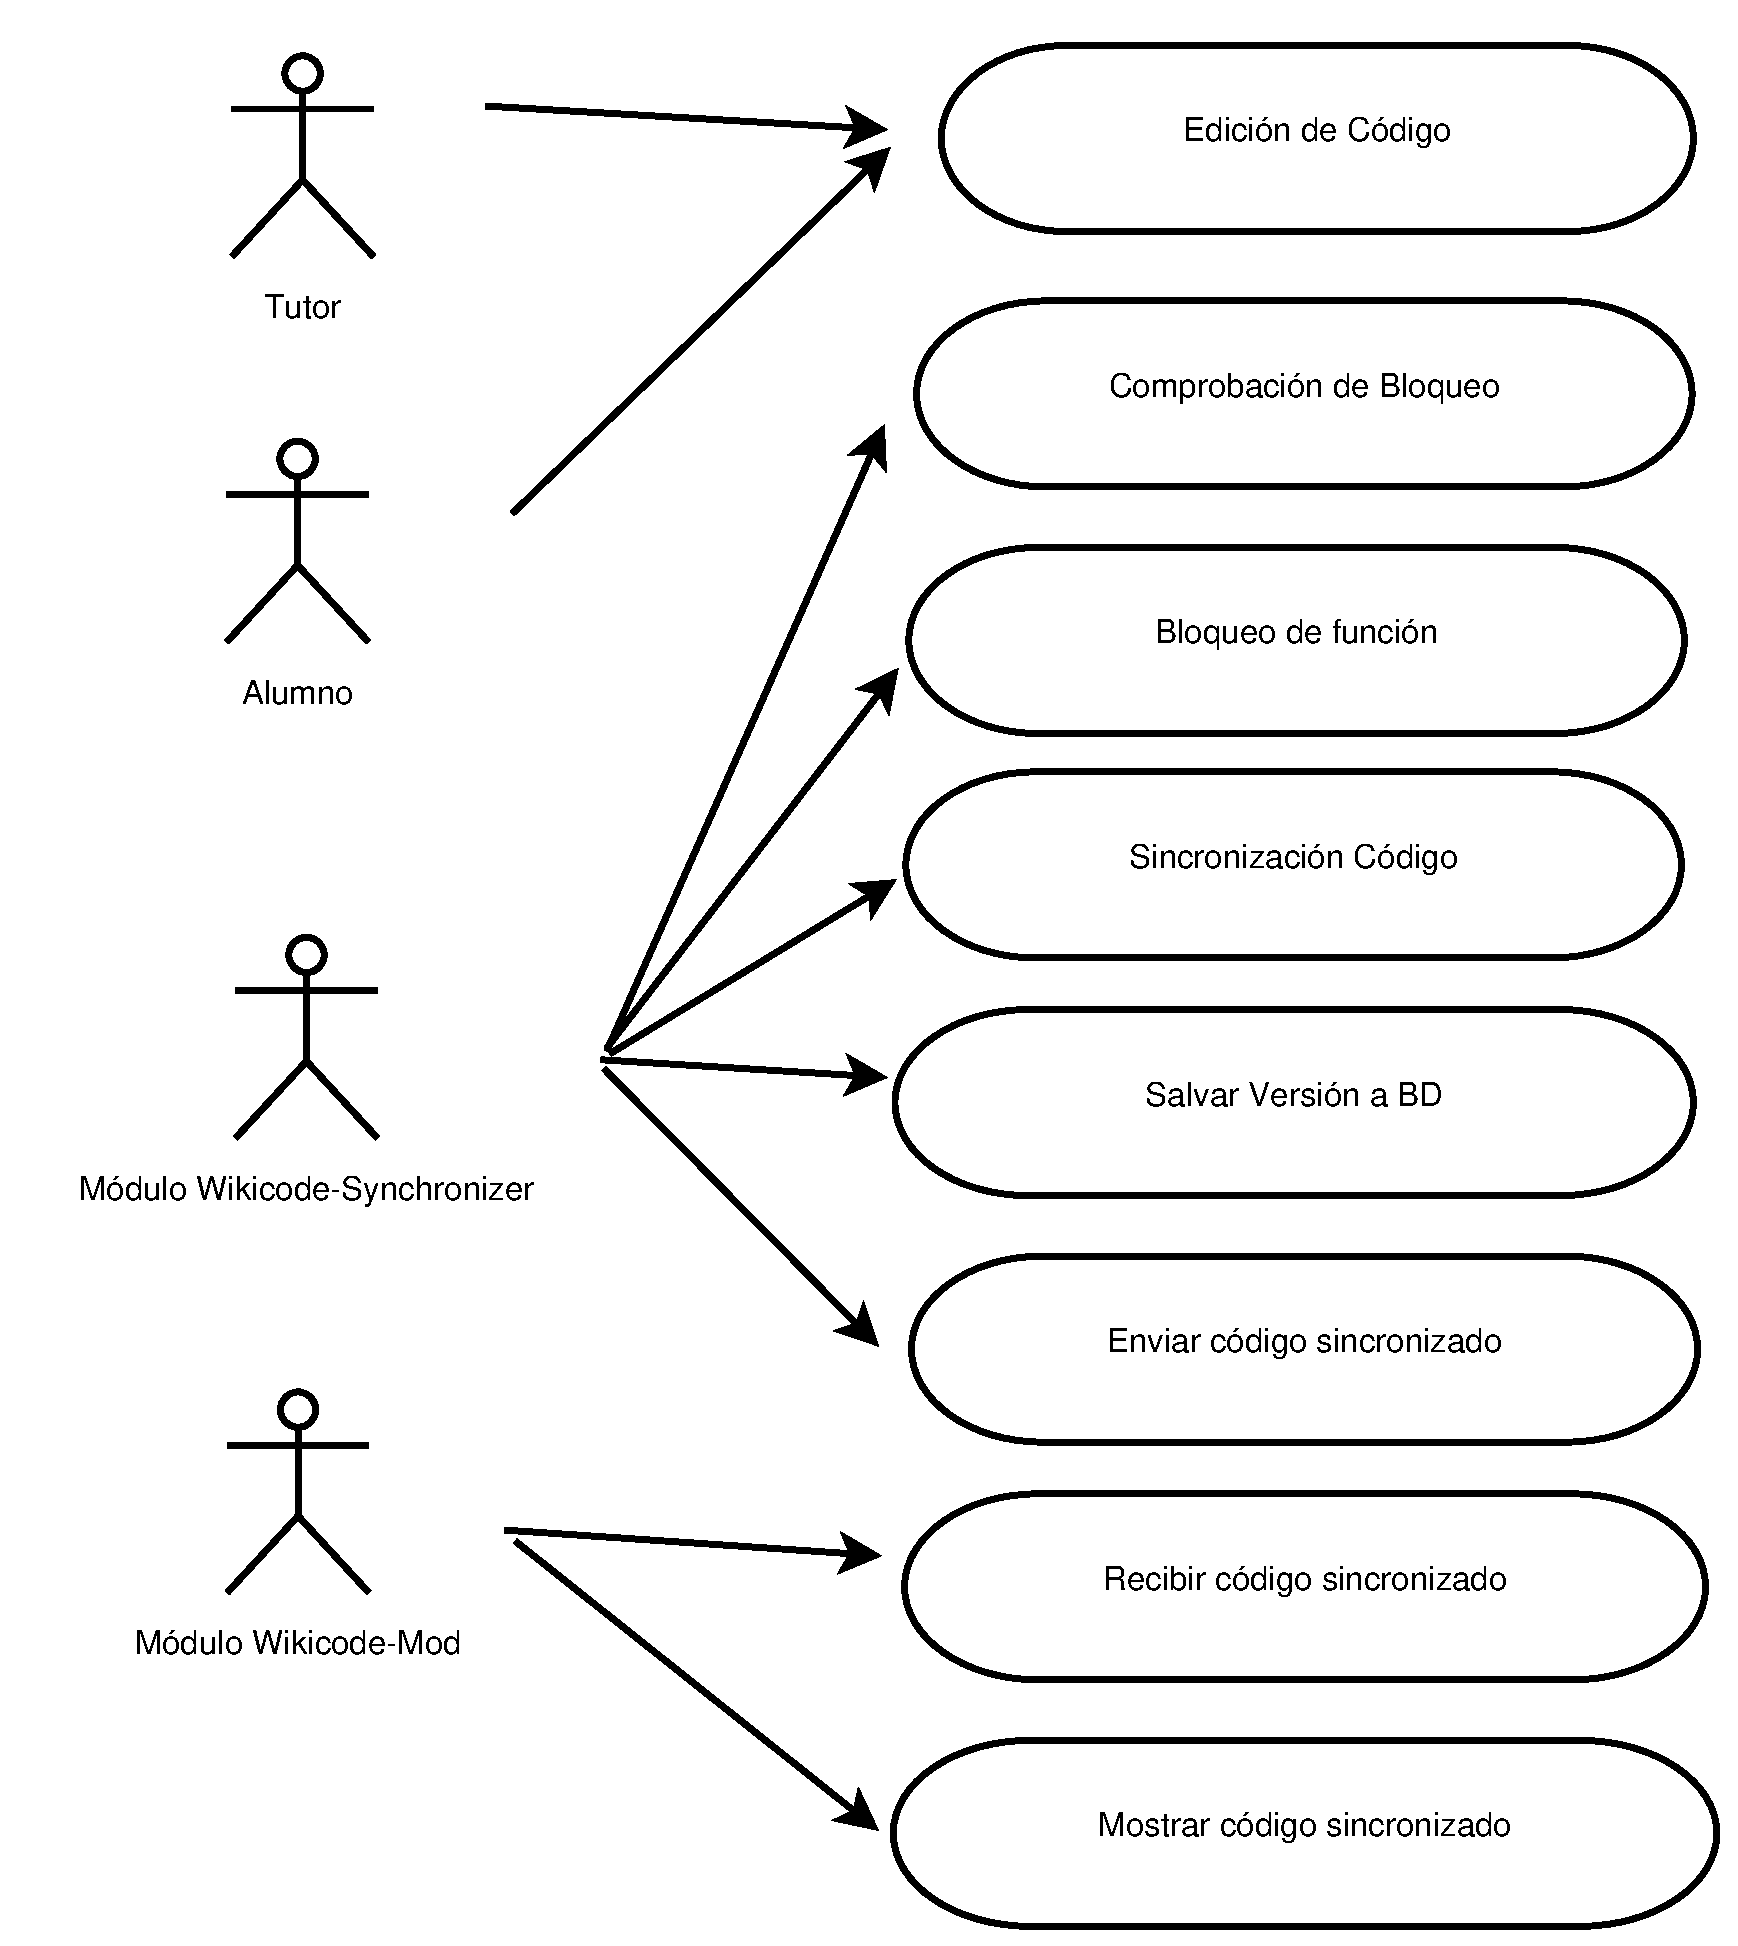
\includegraphics[width=0.5\textwidth]{./img/c3-cu3.eps}
	\caption{Diagrama Caso de uso C3}
\end{figure}

\newpage

\begin{itemize}
	\item Diagrama del Caso de uso C4:
\end{itemize}

\begin{figure}[h]
	\centering
	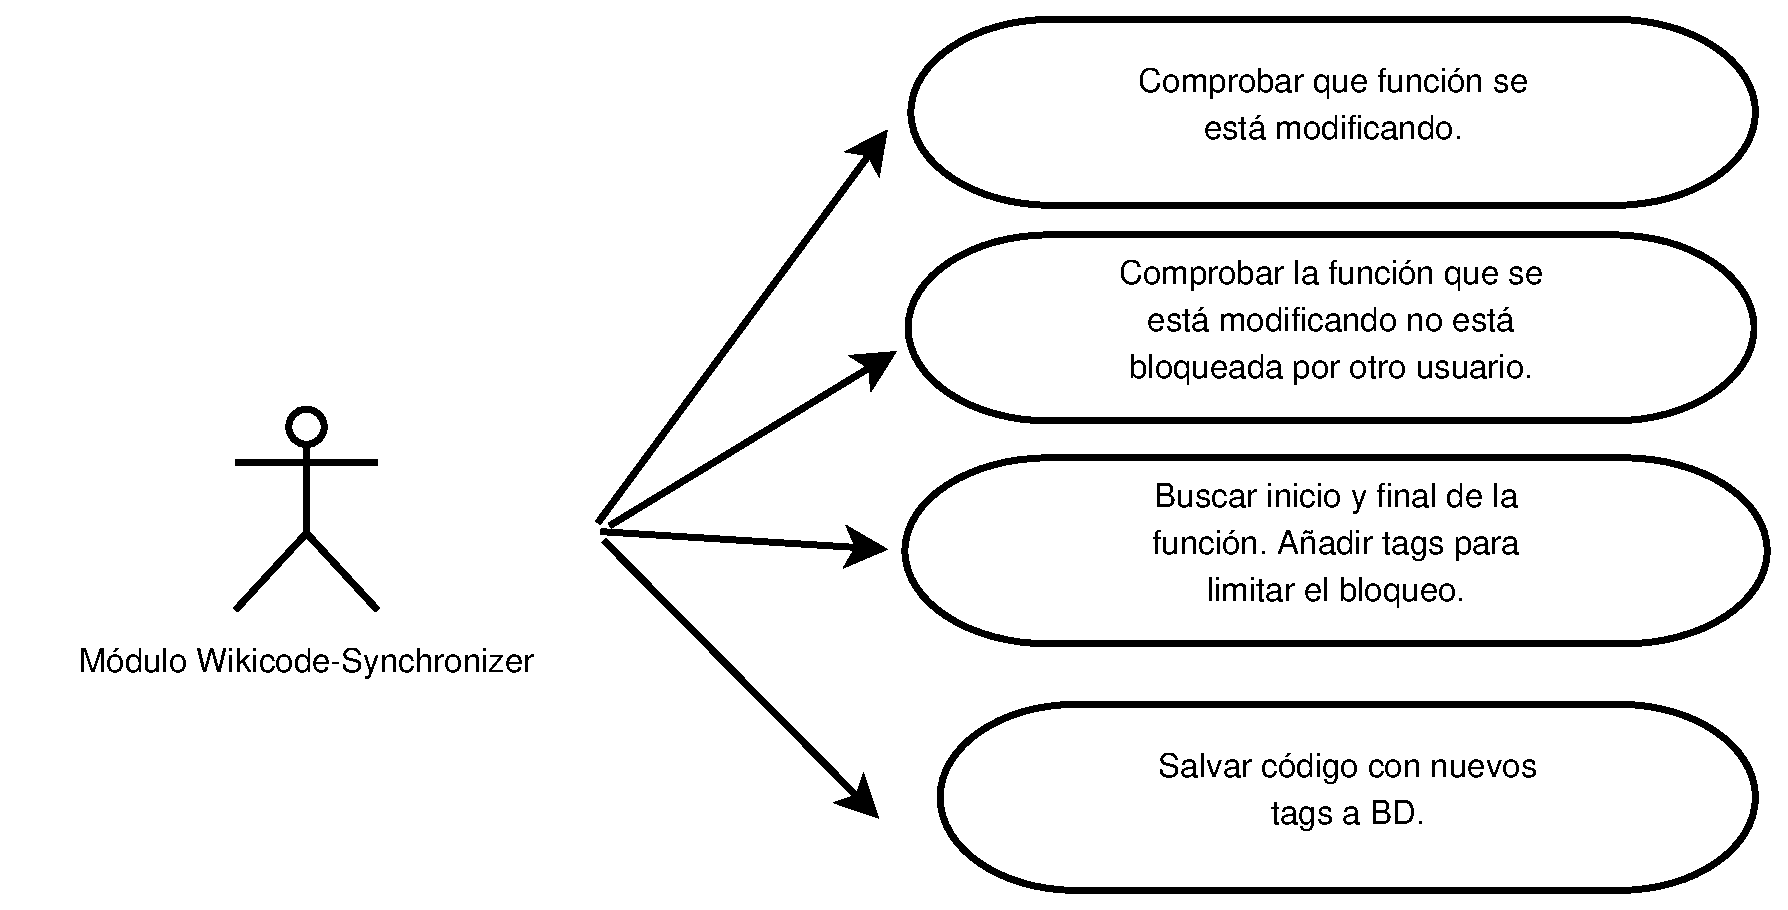
\includegraphics[width=0.5\textwidth]{./img/c3-cu4.eps}
	\caption{Diagrama Caso de uso C4}
\end{figure}

\vspace{1.5cm}

\begin{itemize}
	\item Diagrama del Caso de uso C5:
\end{itemize}

\begin{figure}[h]
	\centering
	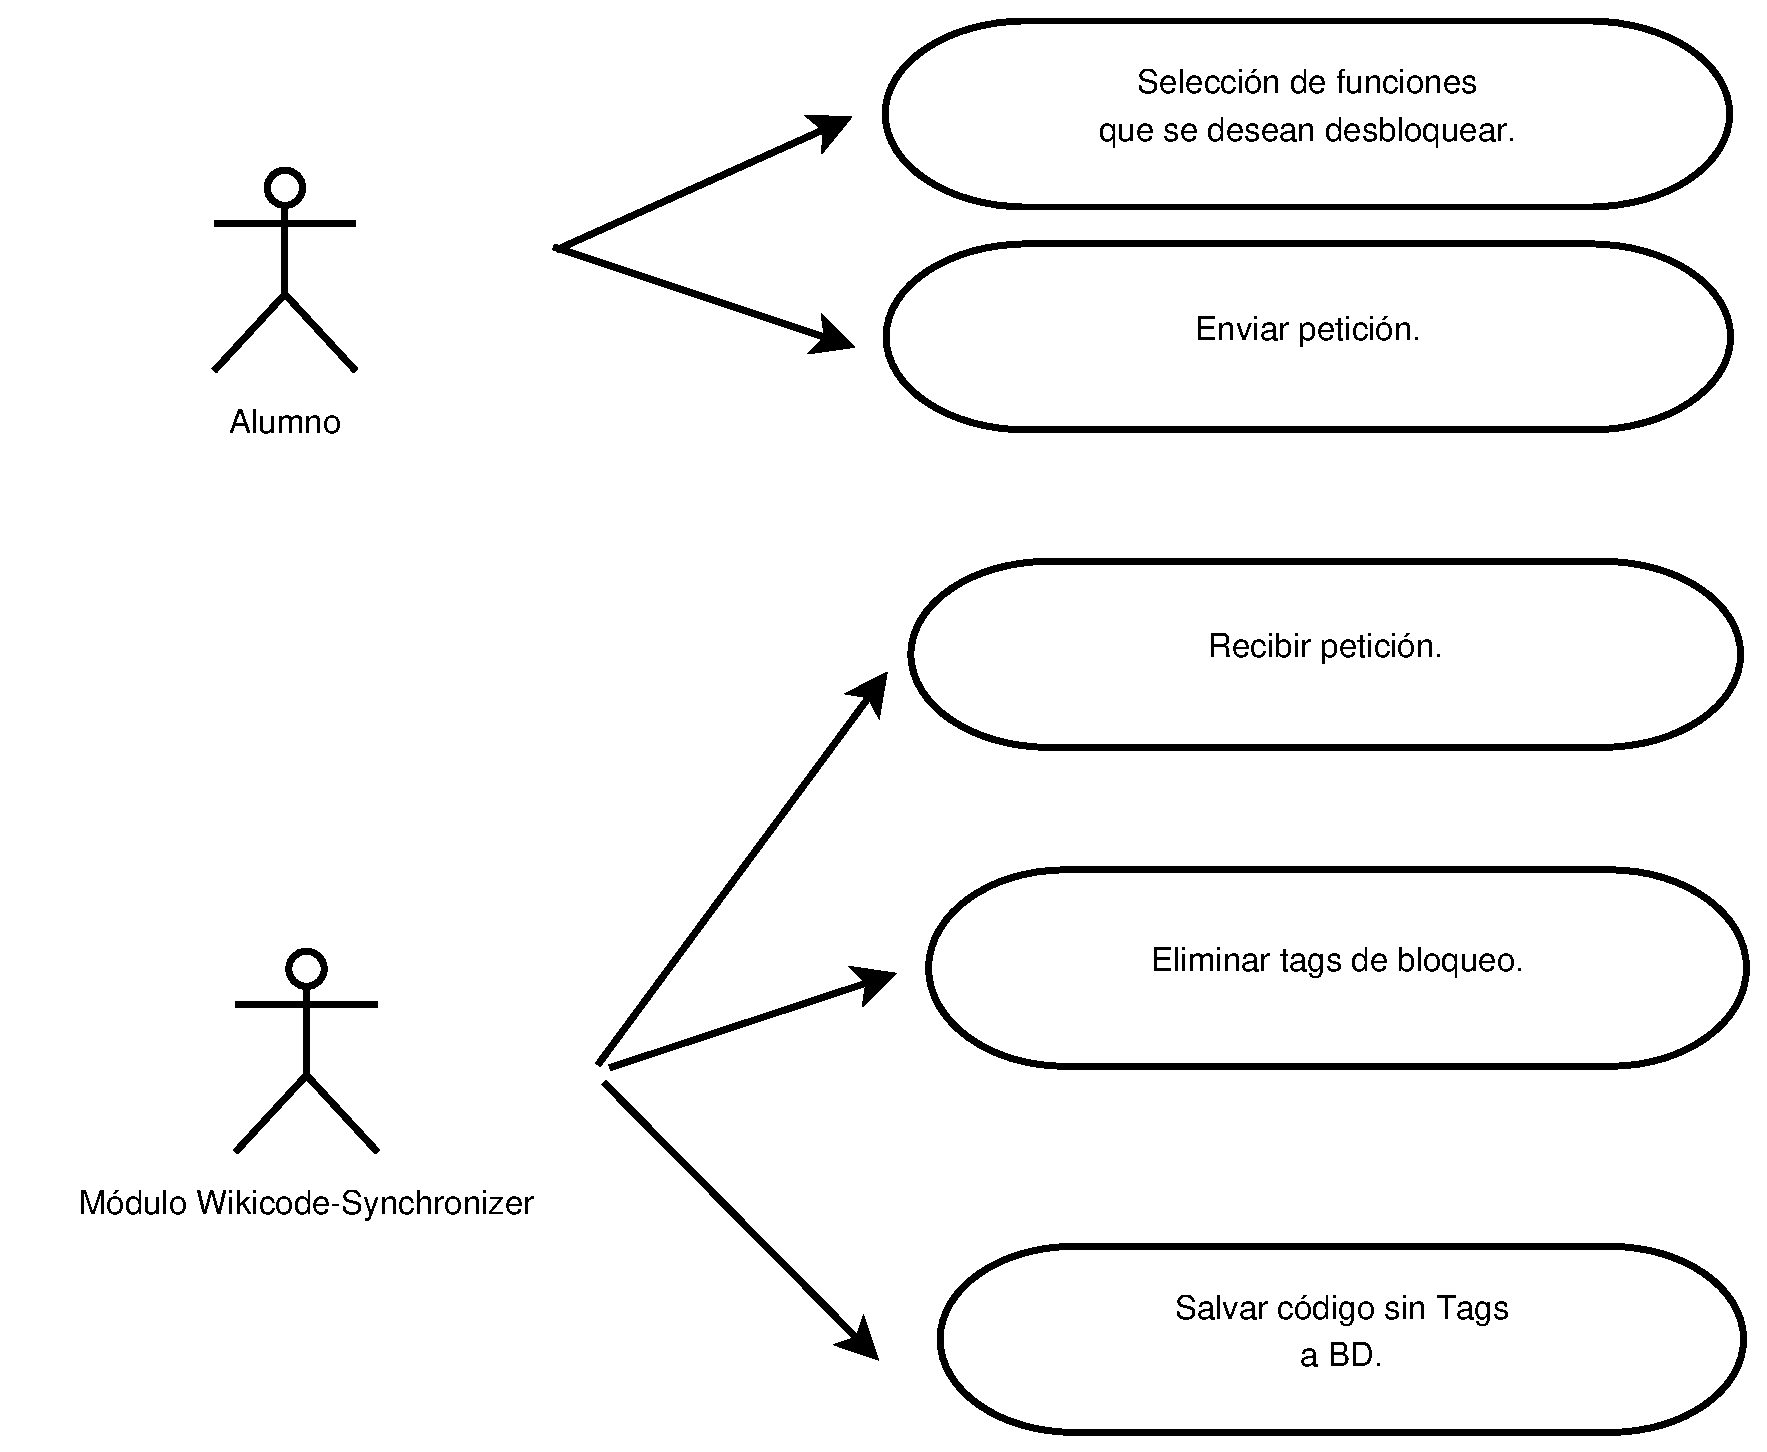
\includegraphics[width=0.5\textwidth]{./img/c3-cu5.eps}
	\caption{Diagrama Caso de uso C5}
\end{figure}

\newpage

\begin{itemize}
	\item Diagrama del Caso de uso C6:
\end{itemize}

\begin{figure}[h]
	\centering
	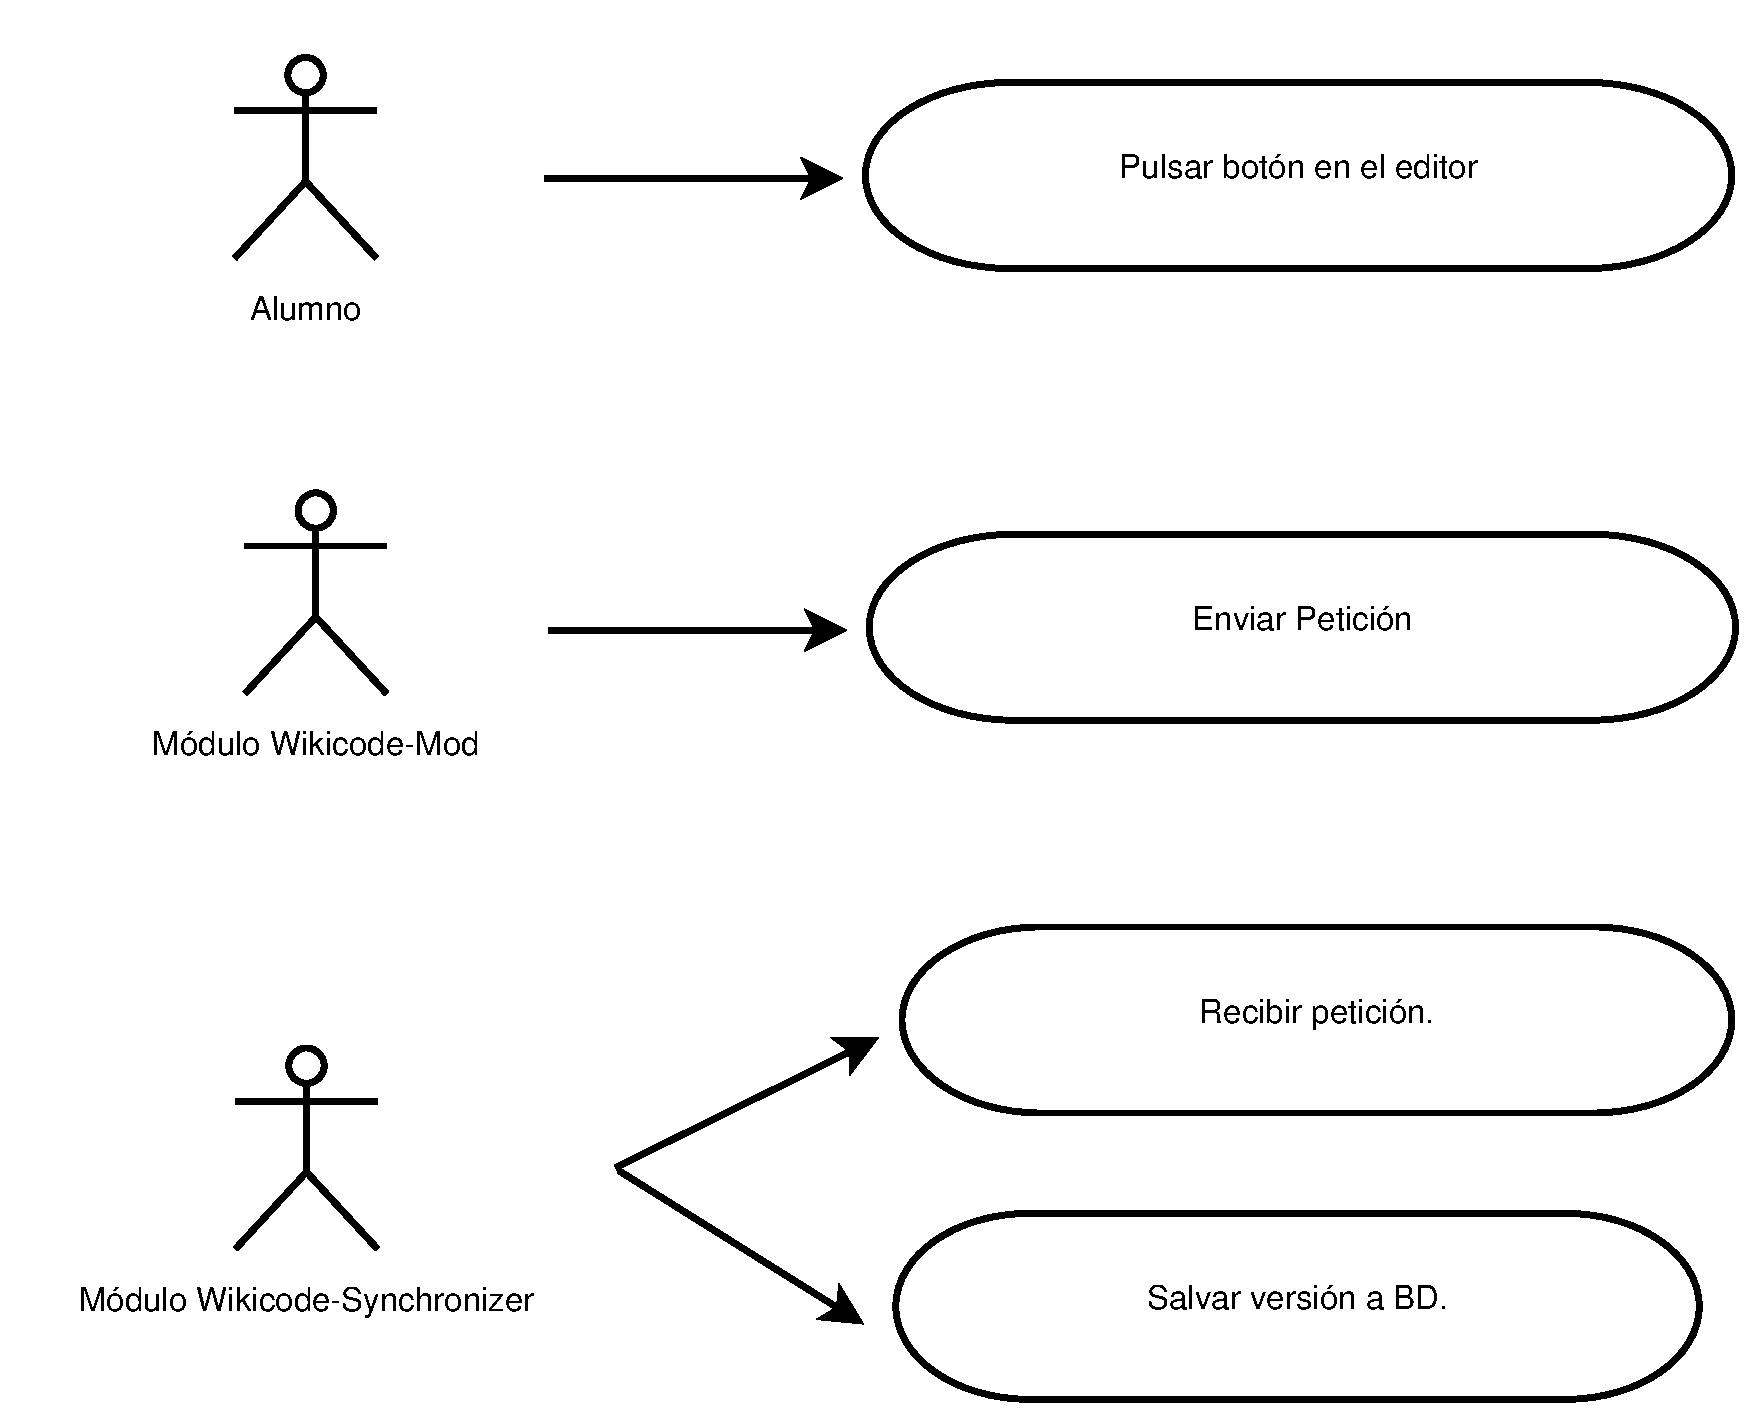
\includegraphics[width=0.5\textwidth]{./img/c3-cu6.eps}
	\caption{Diagrama Caso de uso C6}
\end{figure}

\vspace{1.5cm}

\begin{itemize}
	\item Diagrama del Caso de uso C7:
\end{itemize}

\begin{figure}[h]
	\centering
	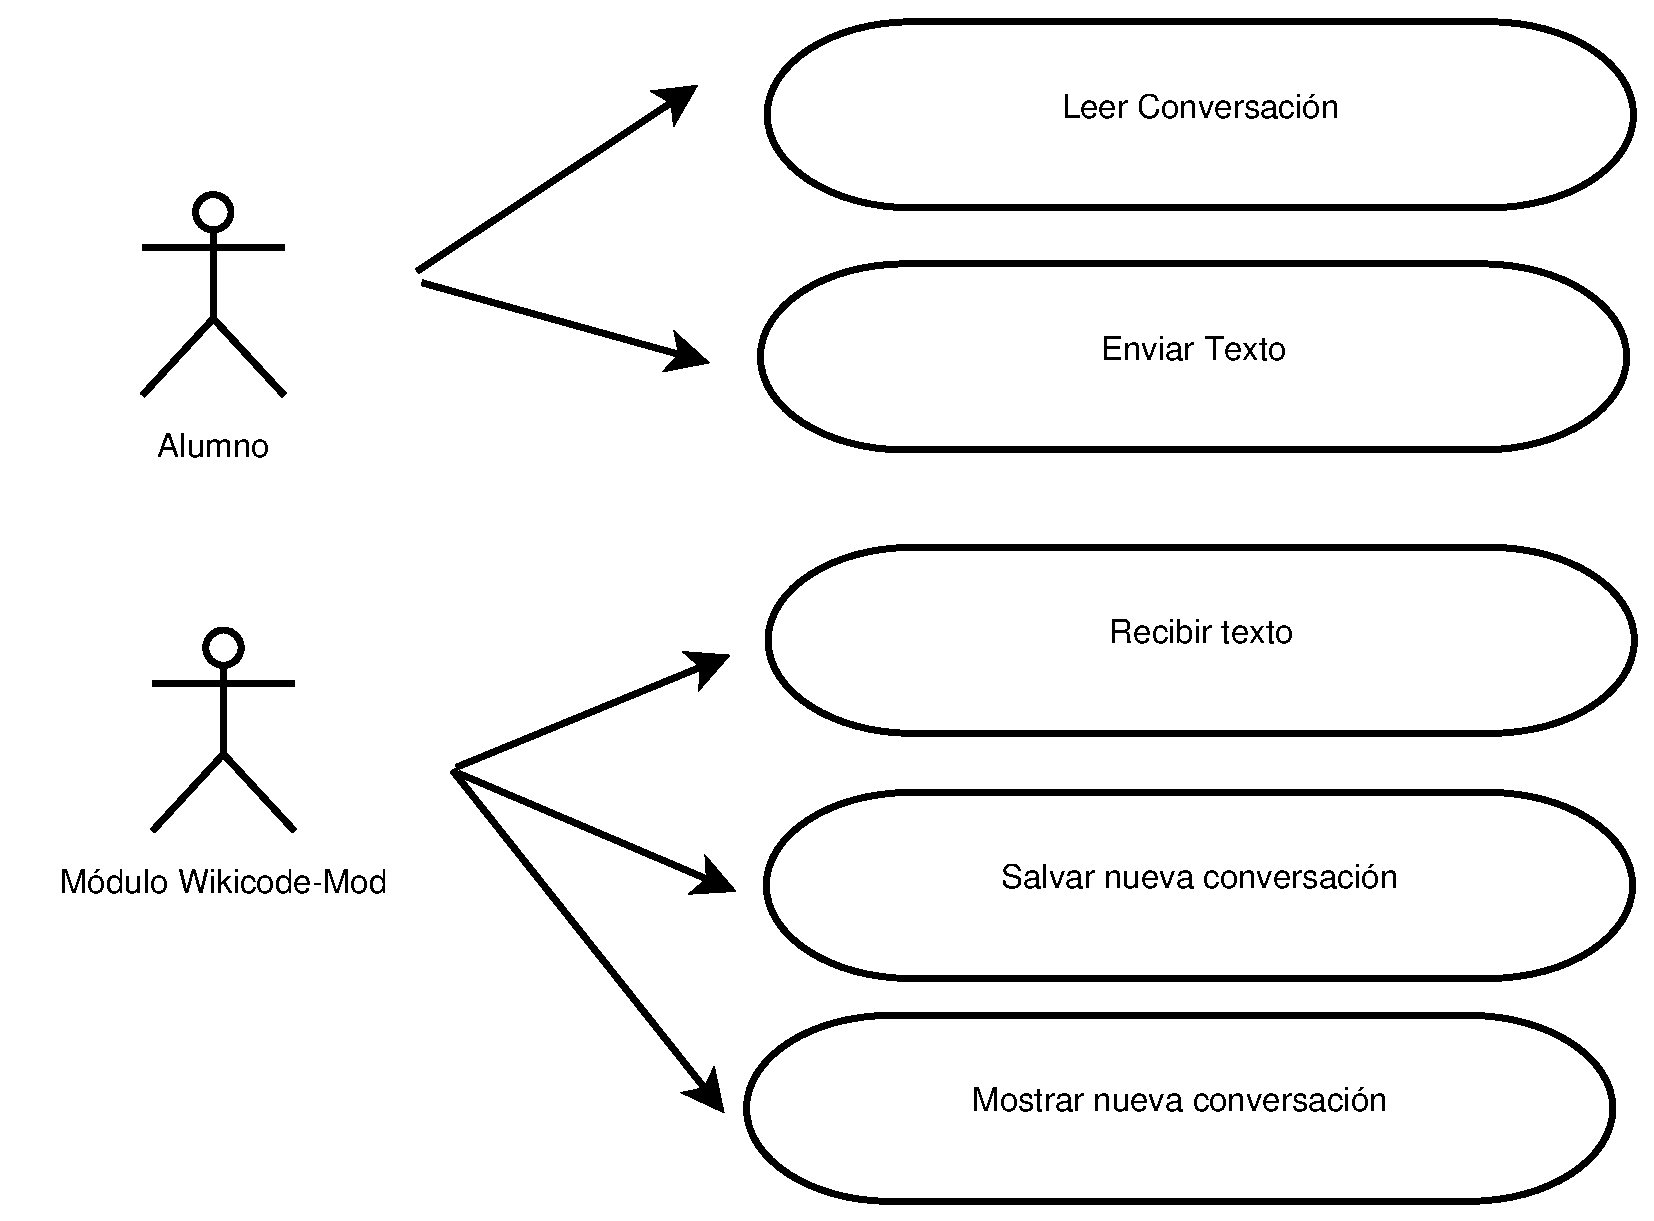
\includegraphics[width=0.5\textwidth]{./img/c3-cu7.eps}
	\caption{Diagrama Caso de uso C7}
\end{figure}

\newpage

\begin{itemize}
	\item Diagrama del Caso de uso C8:
\end{itemize}

\begin{figure}[h]
	\centering
	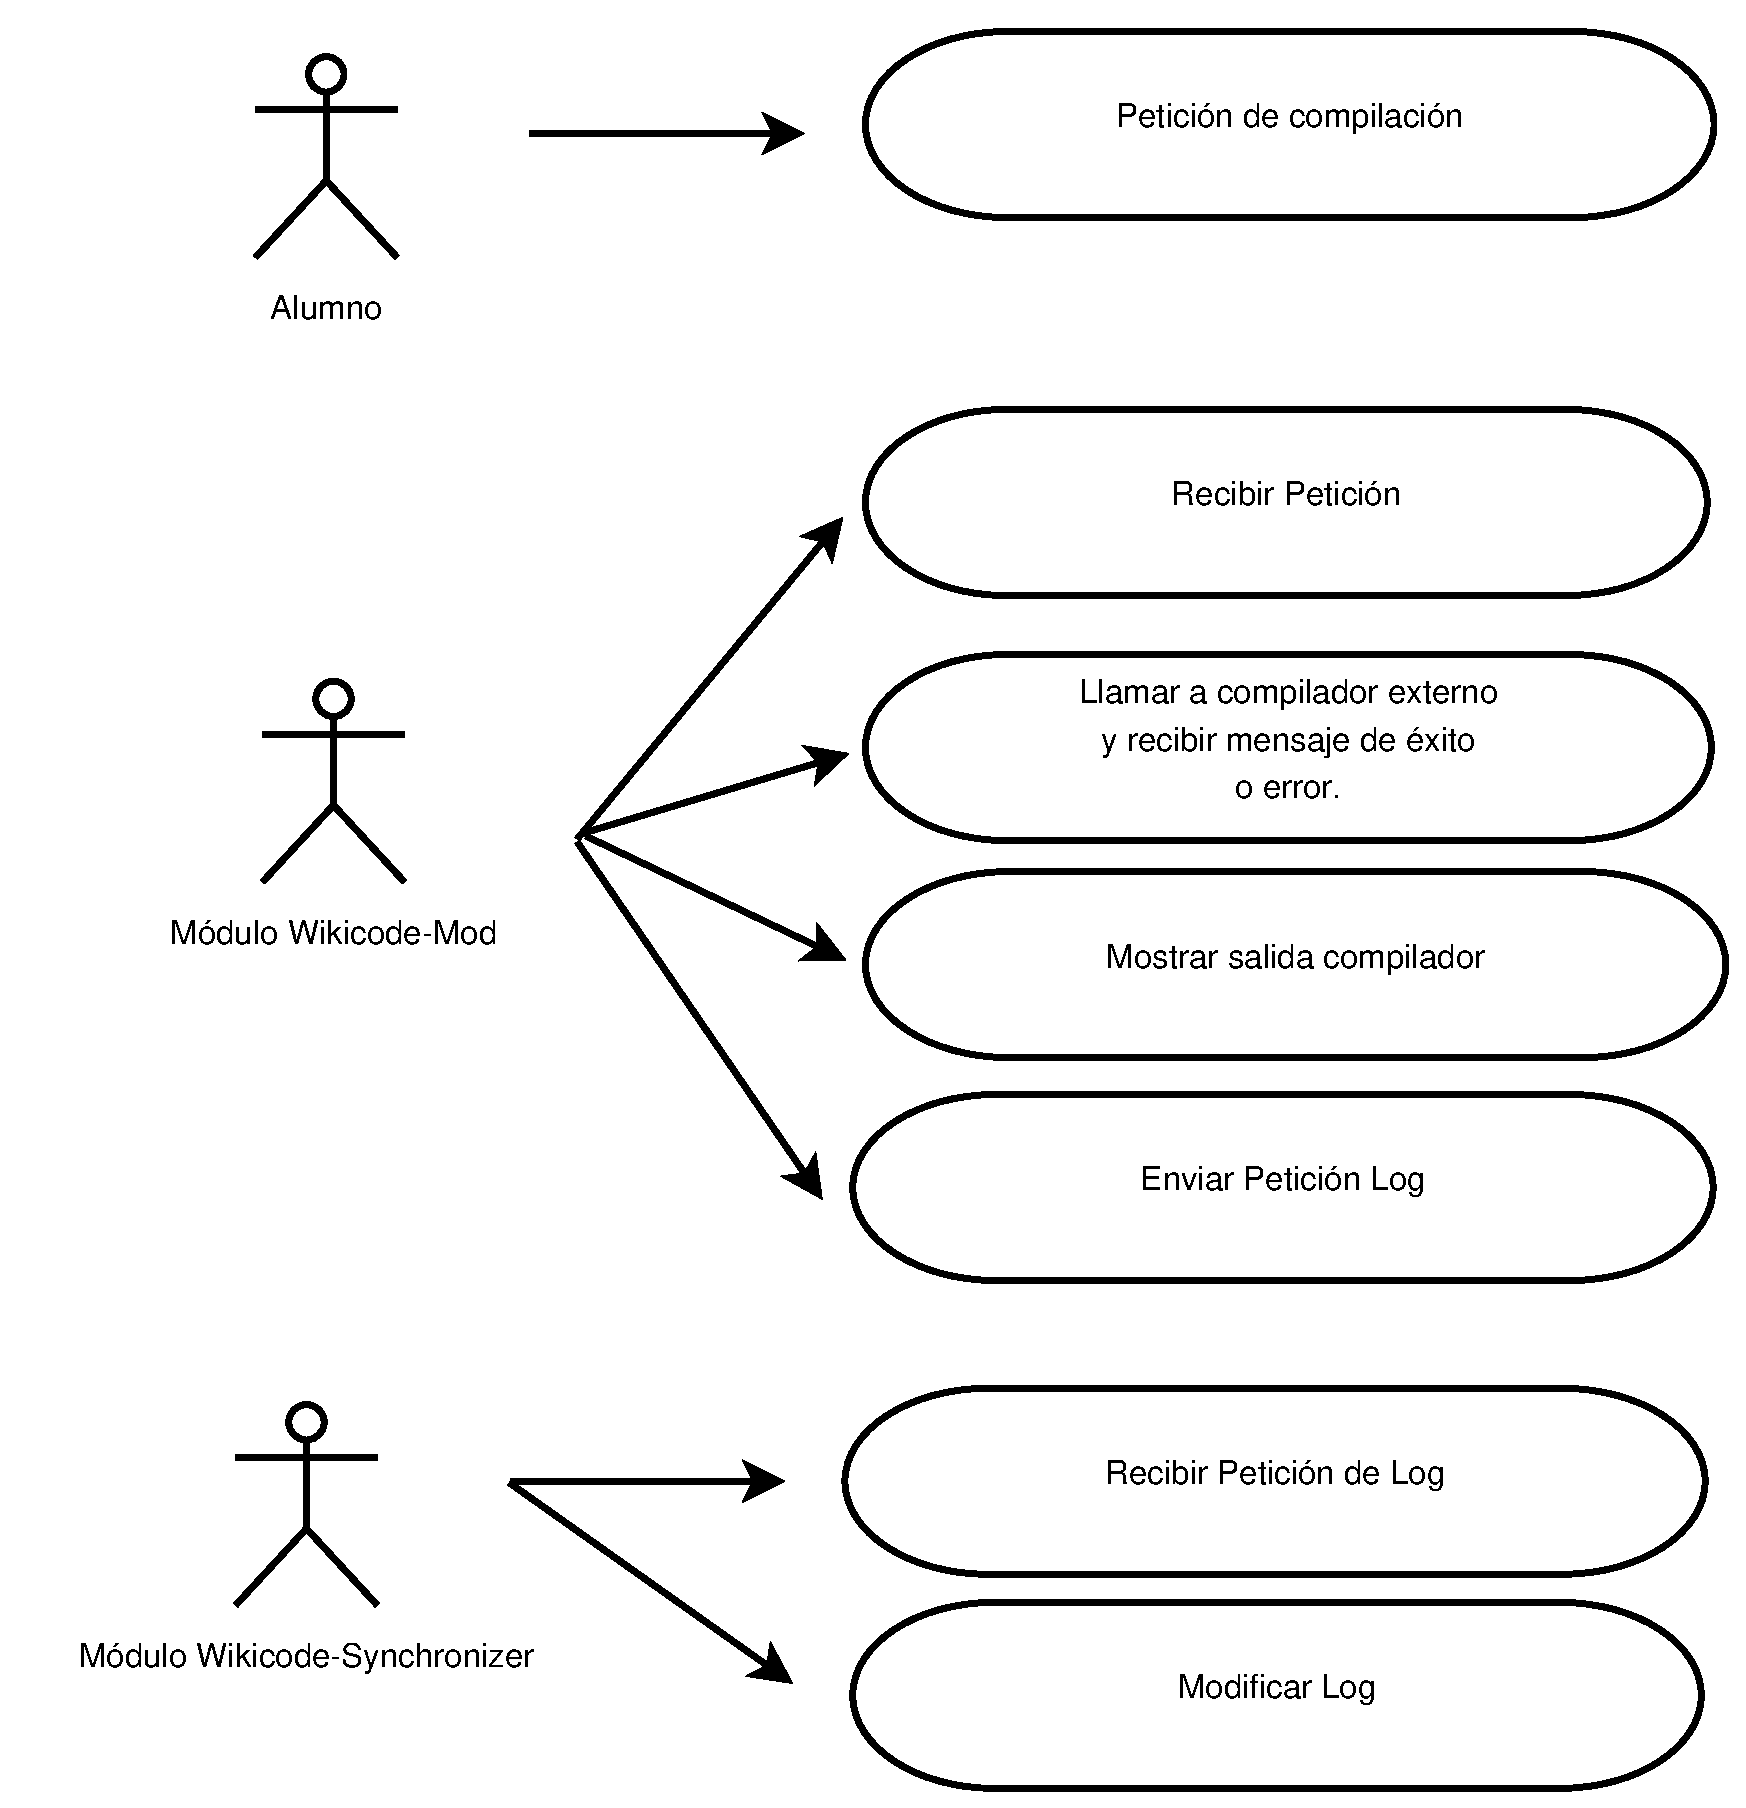
\includegraphics[width=0.5\textwidth]{./img/c3-cu8.eps}
	\caption{Diagrama Caso de uso C8}
\end{figure}

\vspace{1.5cm}

\begin{itemize}
	\item Diagrama del Caso de uso C9:
\end{itemize}

\begin{figure}[h]
	\centering
	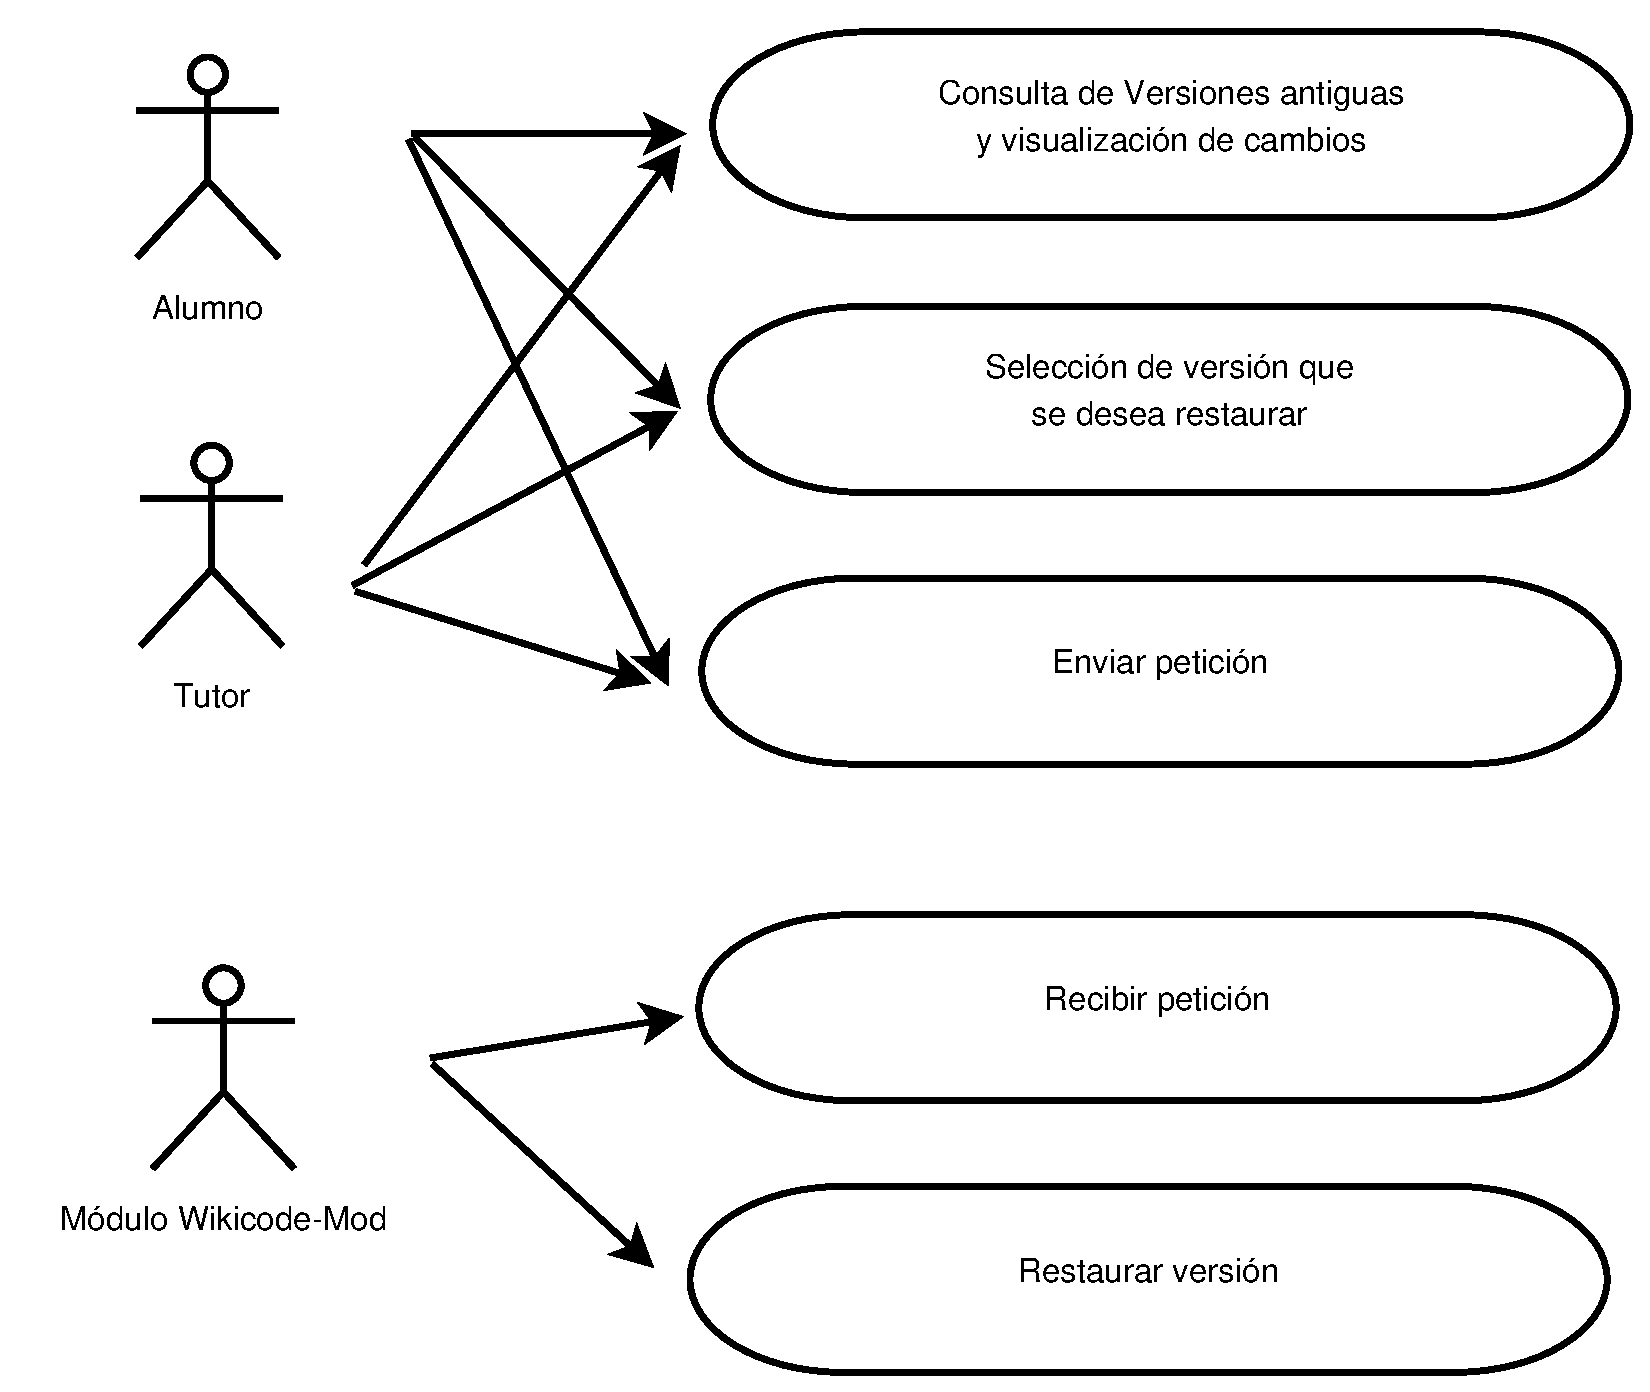
\includegraphics[width=0.5\textwidth]{./img/c3-cu9.eps}
	\caption{Diagrama Caso de uso C9}
\end{figure}

\newpage

\begin{itemize}
	\item Diagrama del Caso de uso C10:
\end{itemize}

\begin{figure}[h]
	\centering
	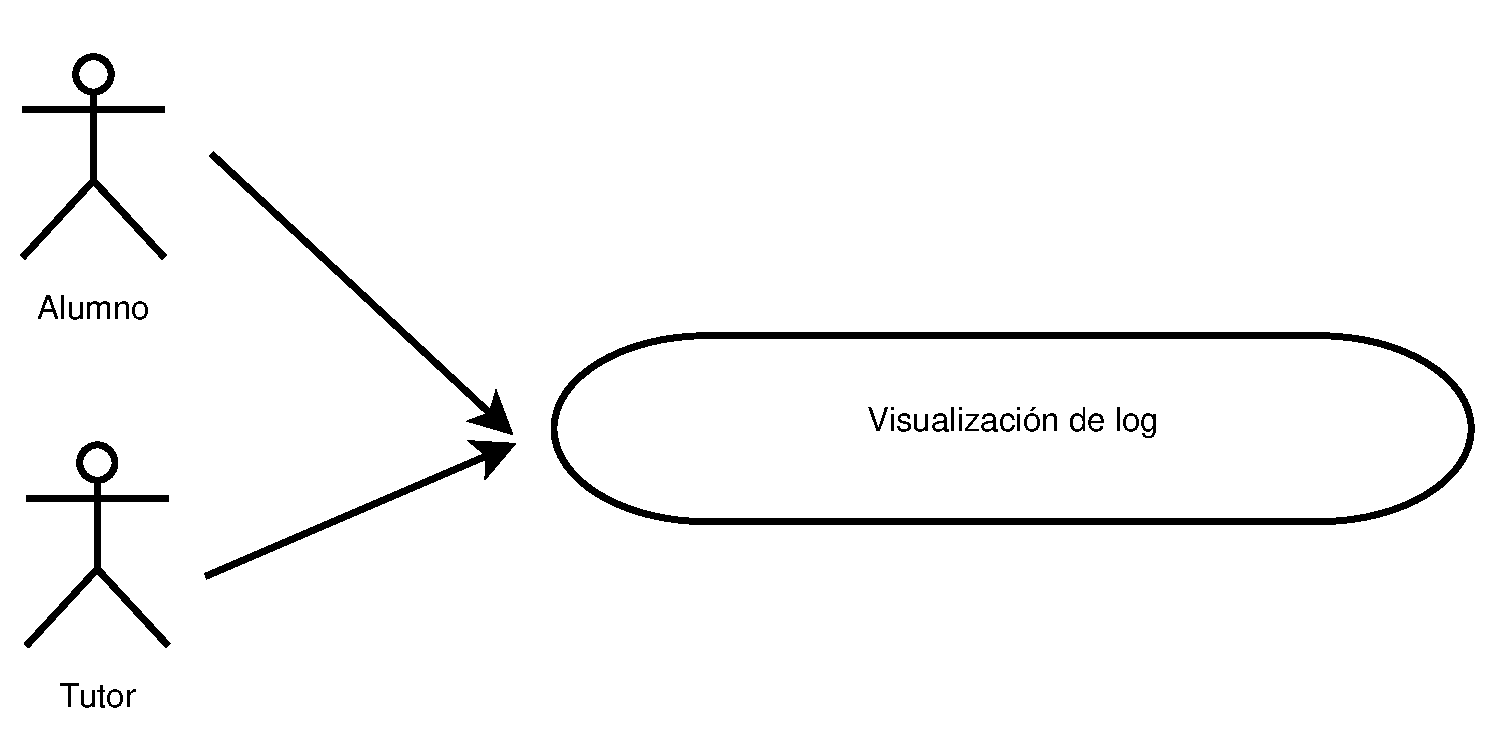
\includegraphics[width=0.5\textwidth]{./img/c3-cu10.eps}
	\caption{Diagrama Caso de uso C10}
\end{figure}

\vspace{2cm}

\subsection{Matriz requisito / Caso de uso}

En la siguiente tabla se describe la matriz de trazabilidad que permite relacionar los casos de uso del sistema con los requerimientos funcionales, permitiendo conocer que requerimientos funcionales resuelve cada caso de uso.

\begin{table}[h]
\centering
\begin{tabular}{ | l | c | c | c | c | c | c | c | c | c | c |}
	\hline
	 & C1 & C2 & C3 &C4 & C5 & C6 & C7 & C8 & C9 & C10 \\
	\hline
	RC1 & X & & & & & & & & & \\
	\hline
	RC2 & X & & & & & & & & &  \\
	\hline
	RC3 & X & & & & & & & & &  \\
	\hline
	RVC1 & & X & & & & & & & &  \\
	\hline
	RVC2 & & X & & & & & & & &  \\
	\hline
	REC1 & & & X & & & & & & &  \\
	\hline
	REC2 & & & X & & & & & & &  \\
	\hline
	REC3 & & & X & & & & & & &  \\
	\hline
	REC4 & & & X & & & & & & &  \\
	\hline
	REC5 & & & X & & & & & & &  \\
	\hline
	REC6 & & & & X & & & & & &  \\
	\hline
	RCH1 & & & & & & & X & & &  \\
	\hline
	RCH2 & & & & & & & X & & &  \\
	\hline
	RCH3 & & & & & & & X & & &  \\
	\hline
	\multicolumn{11}{|c|}{Continua en la siguiente página} \\
	\hline
\end{tabular}
\end{table}

\newpage

\begin{table}[h]
\centering
\begin{tabular}{ | l | c | c | c | c | c | c | c | c | c | c |}
	\hline
	 & C1 & C2 & C3 &C4 & C5 & C6 & C7 & C8 & C9 & C10 \\
	\hline
	RCC1 & & & & & & & & X & &  \\
	\hline
	RCC2 & & & & & & & & X & &  \\
	\hline
	RHC1 & & & & & & & & & X &  \\
	\hline
	RHC2 & & & & & & & & & X &  \\
	\hline
	RLP1 & & & & & & & & & & X  \\
	\hline
	RLP2 & & & & & & & & & & X  \\
	\hline
	RA1 & X & & & & & & & & &  \\
	\hline
	RA2 & X & & & & & & & & &  \\
	\hline
	RSC1 & & & & & & X & & & &  \\
	\hline
	RSC2 & & & & & & X & & & &  \\
	\hline
	RSC3 & & & & & & X & & & &  \\
	\hline
	RSC4 & & & & & & X & & & &  \\
	\hline
	RSC5 & & & & & & X & & & &  \\
	\hline
	RLU1 & & & & X & & & & & &  \\
	\hline
	RLU2 & & & & X & & & & & &  \\
	\hline
	RLU3 & & & & X & & & & & &  \\
	\hline
	RLU4 & & & & & X & & & & &  \\
	\hline
	RAL1 & & & X & & & & & & &  \\
	\hline
	RAL2 & & & & & & & & X & &  \\
	\hline
\end{tabular}
\caption{Matriz requisito / caso de uso}
\end{table}

\newpage

\subsection{Especificación de los casos de uso}

\subsubsection{C1: Caso de uso Creación y Parametrización de la actividad Wikicode}

La especificación del caso de uso C1 quedará especificada en la siguiente tabla:

\begin{table}[h]
\centering
\begin{tabular}{ | p{0.2\textwidth} | p{0.60\textwidth} | }
	\hline
	\cellcolor[gray]{.8}{ID} & C1 \\
	\hline 
	\cellcolor[gray]{.8}{Nombre} & Creación y Parametrización de la actividad Wikicode \\
	\hline
	\cellcolor[gray]{.8}{Descripción} & El \emph{Tutor} crea una nueva actividad Wikicode e introduce las opciones de configuración sobre las que desea trabajar \\
	\hline
	\cellcolor[gray]{.8}{Actores} & Tutor \\
	\hline
	\cellcolor[gray]{.8}{Asunciones} & Acceso correcto a la base de datos y a los ficheros de registro \\
	\hline
	\cellcolor[gray]{.8}{Pasos} & \begin{enumerate}
		\item El \emph{Tutor} selecciona la creación de una nueva actividad Wikicode.
		\item El \emph{Tutor} selecciona los parámetros de configuración que considere oportunos.
		\end{enumerate} \\
	\hline
	\cellcolor[gray]{.8}{Variaciones} & - \\
	\hline
	\cellcolor[gray]{.8}{Requisitos no funcionales} & - \\
	\hline
	\cellcolor[gray]{.8}{Cuestiones} & - \\
	\hline
	
\end{tabular}
\caption{Especificación caso de uso C1}
\end{table}

\newpage
\subsubsection{C2: Caso de uso Visualización del código desarrollado}

La especificación del caso de uso C2 quedará especificada en la siguiente tabla:

\begin{table}[h]
\centering
\begin{tabular}{ | p{0.2\textwidth} | p{0.60\textwidth} | }
	\hline
	\cellcolor[gray]{.8}{ID} & C2 \\
	\hline 
	\cellcolor[gray]{.8}{Nombre} & Visualización del código desarrollado \\
	\hline
	\cellcolor[gray]{.8}{Descripción} &  Tanto el \emph{Tutor} como el \emph{Alumno} pueden acceder a visualizar el código desarrollado en la actividad Wikicode. \\
	\hline
	\cellcolor[gray]{.8}{Actores} & Tutor. Alumno. \\
	\hline
	\cellcolor[gray]{.8}{Asunciones} & Acceso correcto a la base de datos \\
	\hline
	\cellcolor[gray]{.8}{Pasos} & \begin{enumerate}
		\item El \emph{Tutor} o el \emph{Usuario} seleccionan esta opción en el bloque de Moodle correspondiente. 
		\item Se visualiza el código fuente de la Wikicode seleccionada.
		\end{enumerate} \\
	\hline
	\cellcolor[gray]{.8}{Variaciones} & - \\
	\hline
	\cellcolor[gray]{.8}{Requisitos no funcionales} & - \\
	\hline
	\cellcolor[gray]{.8}{Cuestiones} & - \\
	\hline
	
\end{tabular}
\caption{Especificación caso de uso C2}
\end{table}

\newpage
\subsubsection{C3: Caso de uso Edición del código desarrollado}

La especificación del caso de uso C3 quedará especificada en la siguiente tabla:

\begin{table}[h]
\centering
\begin{tabular}{ | p{0.2\textwidth} | p{0.60\textwidth} | }
	\hline
	\cellcolor[gray]{.8}{ID} & C3 \\
	\hline 
	\cellcolor[gray]{.8}{Nombre} &  Edición del código desarrollado\\
	\hline
	\cellcolor[gray]{.8}{Descripción} &  El \emph{Alumno} editará el código en un campo de texto preparado para ello, a su vez el \emph{Tutor} también podrá realizar dicha acción si la considera oportuno. Del mismo modo de manera automática se llamará al subsistema encargado de la sincronización y los bloqueos y devolverá el código actualizado al módulo encargado de llevarlo al interfaz. \\
	\hline
	\cellcolor[gray]{.8}{Actores} & Tutor. Alumno. Módulo Wikicode-Synchronizer. Módulo Wikicode-Mod. \\
	\hline
	\cellcolor[gray]{.8}{Asunciones} & Acceso correcto a la base de datos y a los ficheros de registro. Conexión entre subsistemas mediante el envío de ficheros de tipo JSON. \\
	\hline
	\cellcolor[gray]{.8}{Pasos} & \begin{enumerate}
		\item El \emph{Alumno} o \emph{Tutor} editan una función en el editor de Código. 
		\item El \emph{Alumno} o \emph{Tutor} pulsan una tecla clave: Punto y coma, Intro, Apertura de Corchete, Retroceso.
		\item El \emph{Módulo Wikicode-Mod} detecta esta acción y envía al {Módulo Wikicode-Synchronizer} el código correspondiente al editor y la posición del cursor dentro del código.
		\end{enumerate} \\
	\hline
	\multicolumn{2}{|c|}{Continua en la siguiente página} \\
	\hline
\end{tabular}
\end{table}

\newpage

\begin{table}[h]
\centering
\begin{tabular}{ | p{0.2\textwidth} | p{0.60\textwidth} | }
	\hline
	\cellcolor[gray]{.8}{Pasos} & \begin{enumerate}
		\setcounter{enumi}{3}
		\item El \emph{Módulo Wikicode-Synchronizer} comprueba si la función no está bloqueada, en caso negativo la bloquea, y sincroniza el código con el del resto de usuarios.
		\item El \emph{Módulo Wikicode-Synchronizer} salva el código en base de datos y envía el código sincronizado al \emph{Módulo Wikicode-Mod}.
		\item El \emph{Módulo Wikicode-Mod} recibe el código y actualiza el editor con el código sincronizado al resto de usuarios. 
		\end{enumerate} \\
	\hline
	\cellcolor[gray]{.8}{Variaciones} & - \\
	\hline
	\cellcolor[gray]{.8}{Requisitos no funcionales} & - \\
	\hline
	\cellcolor[gray]{.8}{Cuestiones} & - \\
	\hline
\end{tabular}
\caption{Especificación caso de uso C3}
\end{table}

\newpage

\subsubsection{C4: Caso de uso Bloqueo del código}

La especificación del caso de uso C4 quedará especificada en la siguiente tabla:

\begin{table}[h]
\centering
\begin{tabular}{ | p{0.2\textwidth} | p{0.60\textwidth} | }
	\hline
	\cellcolor[gray]{.8}{ID} & C4 \\
	\hline 
	\cellcolor[gray]{.8}{Nombre} &  Bloqueo del Código\\
	\hline
	\cellcolor[gray]{.8}{Descripción} &  El emph{módulo Wikicode-Synchronizer} recibirá el carácter que se está modificando, buscará a que función pertenece y tras comprobar que esta no está bloqueada la bloqueará para el usuario que ha ordenado la acción.\\
	\hline
	\cellcolor[gray]{.8}{Actores} & Módulo Wikicode-Synchronizer \\
	\hline
	\cellcolor[gray]{.8}{Asunciones} & Acceso correcto a la base de datos \\
	\hline
	\cellcolor[gray]{.8}{Pasos} & \begin{enumerate}
		\item El \emph{Módulo Wikicode-Synchronizer} comprueba que función se está modificando.
		\item Se comprueba que esta función no esté bloqueada por ningún otro usuario, y en caso de que esta condición se cumpla, se delimitan la función mediante la inserción de tags para marcar el inicio y el fin del bloqueo. Dentro de esos tags también se indica el usuario que la ha bloqueada para facilitar las acciones.
		\item Se salva el código con los nuevos tags a la base de datos.
		\end{enumerate} \\
	\hline
	\cellcolor[gray]{.8}{Variaciones} & - \\
	\hline
	\cellcolor[gray]{.8}{Requisitos no funcionales} & - \\
	\hline
	\cellcolor[gray]{.8}{Cuestiones} & - \\
	\hline
	
\end{tabular}
\caption{Especificación caso de uso C4}
\end{table}

\newpage
\subsubsection{C5: Caso de uso Desbloqueo del código}

La especificación del caso de uso C5 quedará especificada en la siguiente tabla:

\begin{table}[h]
\centering
\begin{tabular}{ | p{0.2\textwidth} | p{0.60\textwidth} | }
	\hline
	\cellcolor[gray]{.8}{ID} & C5 \\
	\hline 
	\cellcolor[gray]{.8}{Nombre} &  Desbloqueo de Código\\
	\hline
	\cellcolor[gray]{.8}{Descripción} &  El emph{Alumno} seleccionará las funciones que desea desbloquear de su lista de funciones bloqueadas, las cuales se envían al submódulo encargado de desbloquear el código.  \\
	\hline
	\cellcolor[gray]{.8}{Actores} &  Alumno. Módulo Wikicode-Mod. Módulo Wikicode-Synchronizer.\\
	\hline
	\cellcolor[gray]{.8}{Asunciones} & Acceso correcto a la base de datos. Envío correcto de fichero JSON. \\
	\hline
	\cellcolor[gray]{.8}{Pasos} & \begin{enumerate}
		\item El \emph{Alumno} pulsa el botón correspondiente a la acción de desbloquear.
		\item El \emph{Módulo Wikicode-Mod} muestra al \emph{Alumno} una lista con todas las funciones que tiene bloqueadas. El alumno las selecciona y estas se envían mediante un fichero JSON al \emph{módulo Wikicode-Synchronizer}.
		\item El \emph{Módulo Wikicode-Synchronizer} tras recibir la petición elimina los tags de bloqueo y salva el código a base de datos. 
		\end{enumerate} \\
	\hline
	\cellcolor[gray]{.8}{Variaciones} & - \\
	\hline
	\cellcolor[gray]{.8}{Requisitos no funcionales} & - \\
	\hline
	\cellcolor[gray]{.8}{Cuestiones} & - \\
	\hline
	
\end{tabular}
\caption{Especificación caso de uso C5}
\end{table}

\newpage
\subsubsection{C6: Caso de uso Salvar Código}

La especificación del caso de uso C6 quedará especificada en la siguiente tabla:

\begin{table}[h]
\centering
\begin{tabular}{ | p{0.2\textwidth} | p{0.60\textwidth} | }
	\hline
	\cellcolor[gray]{.8}{ID} & C6 \\
	\hline 
	\cellcolor[gray]{.8}{Nombre} & Salvar Código \\
	\hline
	\cellcolor[gray]{.8}{Descripción} & El \emph{Alumno} hace una llamada al subsistema encargado del módulo Wikicode y este llamará al subsistema que debe salvar el código en base de datos. \\
	\hline
	\cellcolor[gray]{.8}{Actores} &  Alumno. Módulo Wikicode-Mod. Módulo Wikicode-Synchronizer.\\
	\hline
	\cellcolor[gray]{.8}{Asunciones} & Acceso correcto a la base de datos. Envío correcto de fichero JSON. \\
	\hline
	\cellcolor[gray]{.8}{Pasos} & \begin{enumerate}
		\item El \emph{Alumno} selecciona que desea salvar al código y esta es comunicada al \emph{Módulo Wikicode-Mod}.
		\item El \emph{Módulo Wikicode-Mod} prepara un fichero JSON con la información que desea salvar y se envía al \emph{Módulo Wikicode-Mod}. 
		\item Este tras recibir la petición almacena en base de datos una versión del histórico para que pueda ser consultada posteriormente. 
		\end{enumerate} \\
	\hline
	\cellcolor[gray]{.8}{Variaciones} & - \\
	\hline
	\cellcolor[gray]{.8}{Requisitos no funcionales} & - \\
	\hline
	\cellcolor[gray]{.8}{Cuestiones} & - \\
	\hline
	
\end{tabular}
\caption{Especificación caso de uso C6}
\end{table}

\newpage
\subsubsection{C7: Caso de uso Interacción mediante Chat con otros usuarios}

La especificación del caso de uso C7 quedará especificada en la siguiente tabla:

\begin{table}[h]
\centering
\begin{tabular}{ | p{0.2\textwidth} | p{0.60\textwidth} | }
	\hline
	\cellcolor[gray]{.8}{ID} & C7 \\
	\hline 
	\cellcolor[gray]{.8}{Nombre} & Interacción mediante Chat con otros usuarios \\
	\hline
	\cellcolor[gray]{.8}{Descripción} & El \emph{Alumno} leerá la información del chat y, si así lo desea, podrá enviar un mensaje a la conversación. Este mensaje se realizará a través del subsistema \emph{Wikicode-Mod}. \\
	\hline
	\cellcolor[gray]{.8}{Actores} & Alumno. Módulo Wikicode-Mod. \\
	\hline
	\cellcolor[gray]{.8}{Asunciones} & Acceso correcto a los ficheros de registro \\
	\hline
	\cellcolor[gray]{.8}{Pasos} & \begin{enumerate}
		\item El \emph{Módulo Wikicode-Mod} lee el fichero que se corresponde a la Wikicode que estamos trabajando y la muestra en pantalla.  
		\item El \emph{Alumno} lee la conversación y si así lo desea  puede enviar un nuevo mensaje a esta.
		\item El \emph{Módulo Wikicode-Mod} lee el mensaje enviado y modifica el fichero de conversación con el nuevo mensaje.
		\end{enumerate} \\
	\hline
	\cellcolor[gray]{.8}{Variaciones} & - \\
	\hline
	\cellcolor[gray]{.8}{Requisitos no funcionales} & Esta operación se repite cada 5 segundos para actualizar la información. \\
	\hline
	\cellcolor[gray]{.8}{Cuestiones} & - \\
	\hline
	
\end{tabular}
\caption{Especificación caso de uso C7}
\end{table}

\newpage
\subsubsection{C8: Caso de uso Compilación de código fuente}

La especificación del caso de uso C8 quedará especificada en la siguiente tabla:

\begin{table}[h]
\centering
\begin{tabular}{ | p{0.2\textwidth} | p{0.60\textwidth} | }
	\hline
	\cellcolor[gray]{.8}{ID} & C8 \\
	\hline 
	\cellcolor[gray]{.8}{Nombre} & Compilación de código fuente \\
	\hline
	\cellcolor[gray]{.8}{Descripción} & El \emph{Alumno} llamará al compilador a través de un botón. El módulo \emph{Wikicode-Mod} hará una llamada al compilador pasándole como argumento el código fuente y mostrará su salida al usuario. También se aumentará el contador de estadísticas. \\
	\hline
	\cellcolor[gray]{.8}{Actores} &  Alumno. Módulo Wikicode-Mod. Módulo Wikicode-Synchronizer.\\
	\hline
	\cellcolor[gray]{.8}{Asunciones} & Acceso correcto al compilador y a la base de datos. Acceso correcto a los ficheros de intercambio con el compilador. \\
	\hline
	\cellcolor[gray]{.8}{Pasos} & \begin{enumerate}
		\item El \emph{Alumno} pulsa el botón de Compilar y este se comunica con el \emph{módulo Wikicode-Mod}. 
		\item El \emph{módulo Wikicode-Mod} crea un fichero con el código fuente y llama al compilador para que lo tome como parámetro.
		\item El compilador crea un fichero de salida con sus posibles errores y el \emph{módulo Wikicode-Mod} lo lee y se muestra al usuario.
		\item El \emph{módulo Wikicode-Mod} llama al \emph{módulo Wikicode-Synchronizer} para que este aumente las estadísticas correspondientes a la compilación.
		\end{enumerate} \\
	\hline
	\cellcolor[gray]{.8}{Variaciones} & - \\
	\hline
	\cellcolor[gray]{.8}{Requisitos no funcionales} & - \\
	\hline
	\cellcolor[gray]{.8}{Cuestiones} & - \\
	\hline
	
\end{tabular}
\caption{Especificación caso de uso C8}
\end{table}

\newpage
\subsubsection{C9: Caso de uso Consulta de histórico y restauración de versiones}

La especificación del caso de uso C9 quedará especificada en la siguiente tabla:

\begin{table}[h]
\centering
\begin{tabular}{ | p{0.2\textwidth} | p{0.60\textwidth} | }
	\hline
	\cellcolor[gray]{.8}{ID} & C9 \\
	\hline 
	\cellcolor[gray]{.8}{Nombre} & Consulta de histórico y restauración de versiones \\
	\hline
	\cellcolor[gray]{.8}{Descripción} & El \emph{Alumno} o el \emph{Tutor} podrán consultar las versiones antiguas del código y restaurar alguna de ellas si así lo desean. \\
	\hline
	\cellcolor[gray]{.8}{Actores} & Alumno. Tutor. Módulo Wikicode-Mod. \\
	\hline
	\cellcolor[gray]{.8}{Asunciones} & Acceso correcto a la base de datos y a los ficheros de registro \\
	\hline
	\cellcolor[gray]{.8}{Pasos} & \begin{enumerate}
		\item El \emph{Tutor} o el \emph{Usuario} seleccionan esta opción en el bloque de Moodle correspondiente. 
		\item Se visualizan el histórico de la Wikicode seleccionada.
		\item El \emph{Tutor} o el \emph{Usuario} seleccionan una versión y comprueban el código fuente de ésta.
		\item El \emph{Tutor} o el \emph{Usuario} seleccionan si desean restaurar esta versión.
		\item Si la acción anterior ha sido seleccionada como si, el módulo Wikicode-Mod recibe la petición y modifica el código fuente actual por el de la versión más antigua.
		\end{enumerate} \\
	\hline
	\cellcolor[gray]{.8}{Variaciones} & - \\
	\hline
	\cellcolor[gray]{.8}{Requisitos no funcionales} & - \\
	\hline
	\cellcolor[gray]{.8}{Cuestiones} & - \\
	\hline
	
\end{tabular}
\caption{Especificación caso de uso C9}
\end{table}

\newpage
\subsubsection{C10: Caso de uso Consulta de Estadísticas}

La especificación del caso de uso C10 quedará especificada en la siguiente tabla:

\begin{table}[h]
\centering
\begin{tabular}{ | p{0.2\textwidth} | p{0.60\textwidth} | }
	\hline
	\cellcolor[gray]{.8}{ID} & C10 \\
	\hline 
	\cellcolor[gray]{.8}{Nombre} & Consulta de Estadísticas \\
	\hline
	\cellcolor[gray]{.8}{Descripción} & El \emph{Alumno} o el \emph{Tutor} podrán consultar las estadísticas del código. \\
	\hline
	\cellcolor[gray]{.8}{Actores} & Alumno. Tutor. \\
	\hline
	\cellcolor[gray]{.8}{Asunciones} & Acceso correcto a la base de datos y a los ficheros de registro \\
	\hline
	\cellcolor[gray]{.8}{Pasos} & \begin{enumerate}
		\item El \emph{Tutor} o el \emph{Usuario} seleccionan esta opción en el bloque de Moodle correspondiente. 
		\item Se visualizan las estadísticas de la Wikicode seleccionada.
		\end{enumerate} \\
	\hline
	\cellcolor[gray]{.8}{Variaciones} & - \\
	\hline
	\cellcolor[gray]{.8}{Requisitos no funcionales} & - \\
	\hline
	\cellcolor[gray]{.8}{Cuestiones} & - \\
	\hline
	
\end{tabular}
\caption{Especificación caso de uso C10}
\end{table}

\section{Modelo conceptual}

Para analizar el modelo conceptual realizado se comentarán las diferentes clases que se han desarrollado y se mostrará el diagrama de clases resultante. Como se indicó en apartados anteriores, el proyecto se encuentra fundamentalmente dividido en dos grandes módulos o sistemas. Por tanto, las clases serán explicadas por separado y se realizará un diagrama de clases para cada uno de los sistemas.

De esta manera, una vez extraídas las clases necesarias y suficientes, se va a definir, primeramente, un diccionario de datos expresando el significado concreto de cada clase para evitar posibles interpretaciones erróneas. Como tenemos dos sistemas bien diferenciados, se definirá un diccionario de datos para cada uno de ellos.

\subsection{Diccionario de datos para el sistema Wikicode-Mod}

Este sistema está compuesto por varias clases, las cuales hacen de interfaz entre el usuario y el sistema. Se puede dividir según las opciones que se van a utilizar:

\subsubsection{Class mod\_wikicode\_renderer}

\begin{itemize}
	\item Descripción: Se trata de una clase que genera el interfaz gráfico del módulo a través de un modelo previamente creado.
	\item Observaciones: Esta clase se utiliza para que el módulo Wikicode tenga una apariencia similar a la del resto de módulos Moodle. Hereda de la clase base de moodle encargada del renderizado y se sobrecarga una serie de funciones.
	\item Atributos: No tiene atributos.
	\item Operaciones:
		\begin{itemize}
			\item \textbf{page\_index: }Devuelve el código HTML de una página principal con el formato de Moodle.
			\item \textbf{search\_result: } Devuelve el código HTML de una búsqueda con el formato de Moodle.
			\item \textbf{diff: }Devuelve el código HTML con la diferencia en el contenido de dos Wikicodes.
			\item \textbf{diff\_paging\_bar: } Devuelve el código HTML para proveernos acceso a otras versiones.
			\item \textbf{wikicode\_info: }Devuelve el código HTML de un cuadro con información sobre la Wikicode.
			\item \textbf{tabs: }Devuelve el código HTML de un menú superior con las opciones de navegación de una Wikicode.
			\item \textbf{wikicode\_print\_subwiki\_selector: }Devuelve el código HTML de un menú con las opciones de navegación entre distintas Wikicodes.
			\item \textbf{menu\_admin: }Devuelve el código HTML del menú que se mostrará en caso de que el usuario tenga rol de administrador a la hora de navegar por una Wikicode.
		\end{itemize}
	\item Relaciones:
		\begin{itemize}
			\item \textbf{plugin\_renderer\_base: } Hereda de esta clase.
		\end{itemize}
	\newpage
	\item Diagrama de la clase:
		\begin{figure}[h]
			\centering
			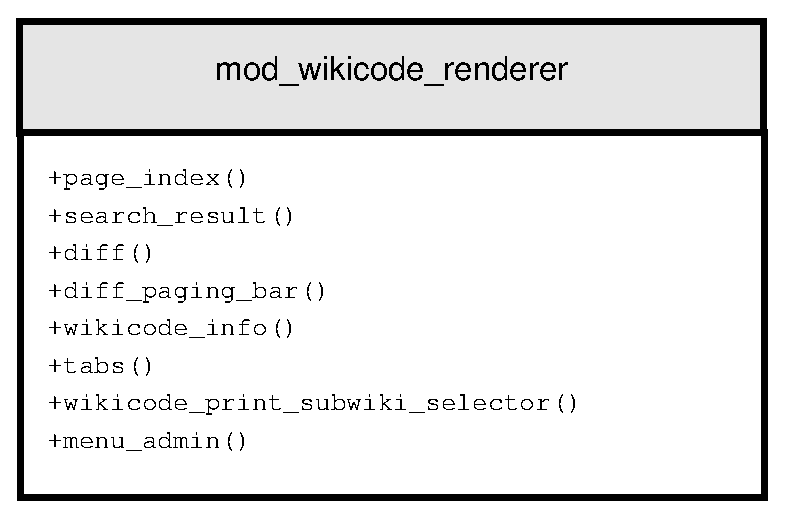
\includegraphics[width=0.5\textwidth]{./img/mod_wikicode_renderer.eps}
			\caption{Class mod\_wikicode\_renderer}
		\end{figure}
\end{itemize}

\subsubsection{class page\_wikicode}

\begin{itemize}
	\item Descripción: Contiene el código común entre todos los tipos de páginas
	\item Observaciones: Se trata de una clase abstracta que sirve de interfaz para el resto de clases que van a crear una página.
	\item Atributos:
		\begin{itemize}
			\item subwiki:
				\begin{itemize}
					\item Descripción: Identificador de la Wiki actualmente seleccionada.
					\item Dominio: Variable de tipo entero.
				\end{itemize}
			\item page:
				\begin{itemize}
					\item Descripción: Identificador de la página Wiki actualmente seleccionada.
					\item Dominio: Variable de tipo entero.
				\end{itemize}
			\item title:
				\begin{itemize}
					\item Descripción: Título de la página actual.
					\item Dominio: Variable de tipo string.
				\end{itemize}
			\item gid:
				\begin{itemize}
					\item Descripción: Identificador del grupo actualmente seleccionado.
					\item Dominio: Variable de tipo entero.
				\end{itemize}
			\item modcontext:
				\begin{itemize}
					\item Descripción: Contexto del módulo.
					\item Dominio: Variable de tipo objeto.
				\end{itemize}
			\item uid:
				\begin{itemize}
					\item Descripción: Identificador del usuario actual.
					\item Dominio: Variable de tipo entero.
				\end{itemize}
			\item tabs:
				\begin{itemize}
					\item Descripción: Objeto con las opciones que son mostradas en el menú superior.
					\item Dominio: Variable de tipo objeto.
				\end{itemize}
			\item tabs\_options:
				\begin{itemize}
					\item Descripción: Objeto con las opciones del menú superior.
					\item Dominio: Variable de tipo objeto.
				\end{itemize}
			\item wikioutput:
				\begin{itemize}
					\item Descripción: Objeto con las opciones de renderizado del módulo Wikicode seleccionado.
					\item Dominio: Variable de tipo objeto.
				\end{itemize}
		\end{itemize}
	\item Operaciones:
		\begin{itemize}
			\item \textbf{print\_header: }Esta operación devuelve el código HTML que imprime la parte superior de la página.
			\item \textbf{print\_pagetitle: }Método para imprimir el título de la página.
			\item \textbf{setup\_tabs: }Método para configurar el menú superior y dejar marcada la opción sobre la que estamos navegando.
			\item \textbf{print\_content: }Operación que debe ser sobrescrita por las clases que hereden de esta para imprimir el código HTML correspondiente al cuerpo central de la página.
			\item \textbf{set\_page: }Método para asignar la página actual.
			\item \textbf{set\_title: }Método para asignar el título de la página actual.
			\item \textbf{set\_gid: }Método para asignar el identificador de grupo.
			\item \textbf{set\_uid: }Método para asignar el identificador de usuario.
			\item \textbf{print\_footer: }Esta operación devuelve el código HTML que imprime la parte inferior de la página.
			\item \textbf{set\_session\_url: }Operación para indicar a la variable global de Moodle \$SESSION la página web actual sobre la que estamos navegando.
			\item \textbf{print\_tab: }Imprime el menú superior con las opciones configuradas en la página.
		\end{itemize}
	\item Relaciones:
		\begin{itemize}
			\item \textbf{page\_wikicode\_view: } Padre de esta clase.
			\item \textbf{page\_wikicode\_edit: } Padre de esta clase.
			\item \textbf{page\_wikicode\_log: } Padre de esta clase.
			\item \textbf{page\_wikicode\_search: } Padre de esta clase.
			\item \textbf{page\_wikicode\_create: } Padre de esta clase.
			\item \textbf{page\_wikicode\_diff: } Padre de esta clase.
			\item \textbf{page\_wikicode\_history: } Padre de esta clase.
			\item \textbf{page\_wikicode\_restoreversion: } Padre de esta clase.
			\item \textbf{page\_wikicode\_viewversion: } Padre de esta clase.
			\item \textbf{page\_wikicode\_admin: } Padre de esta clase.
		\end{itemize}
	\item Diagrama de la clase:
		\begin{figure}[h]
			\centering
			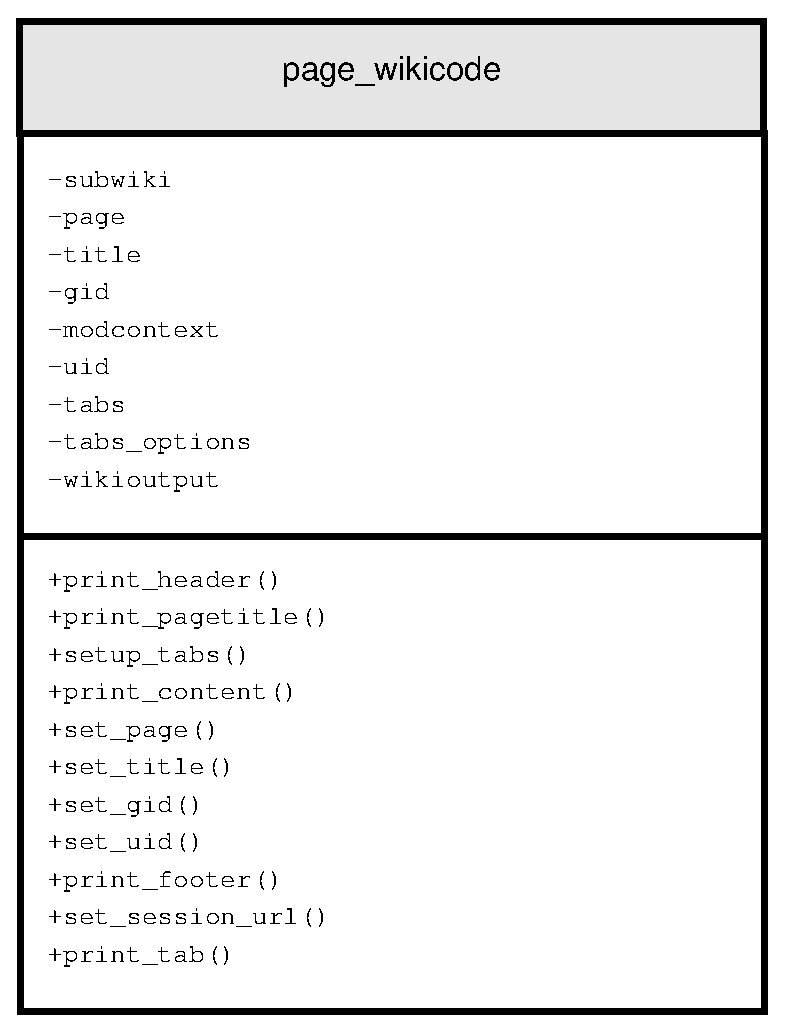
\includegraphics[width=0.5\textwidth]{./img/page_wikicode.eps}
			\caption{Class page\_wikicode}
		\end{figure}
\end{itemize}

\subsubsection{Class page\_wikicode\_view}

\begin{itemize}
	\item Descripción: Clase para mostrarnos una página de Wikicode en la que se muestra el código fuente como texto plano.
	\item Observaciones: Se considera que esta clase es la que hace de interfaz en el caso de uso \emph{Visualización de código desarrollado}.
	\item Atributos:
		\begin{itemize}
			\item coursemodule:
				\begin{itemize}
					\item Descripción: Identificar del curso sobre el que está creado la Wikicode.
					\item Dominio: Variable de tipo entero.
				\end{itemize}
		\end{itemize}
	\item Operaciones:
		\begin{itemize}
			\item \textbf{print\_header: }Esta operación devuelve el código HTML que imprime la parte superior de la página.
			\item \textbf{wikicode\_print\_subwiki\_selector: }Esta operación devuelve el código HTML con el menú para seleccionar sobre que Wikicode queremos trabajar.
			\item \textbf{print\_content: }Operación devuelve el código HTML que imprime la parte central de la página.
			\item \textbf{set\_url: }Operación que modifica las variables globales para indicar a Moodle en que página nos encontramos.
			\item \textbf{set\_course\_module: }Método para asignar el identificador de curso de la clase.
			\item \textbf{create\_navbar: }Método para añadir al menú de navegación la opción de Vista.
		\end{itemize}
	\item Relaciones:
		\begin{itemize}
			\item \textbf{page\_wikicode:} Hereda de esta clase.
		\end{itemize}
	\newpage
	\item Diagrama de la clase:
		\begin{figure}[h]
			\centering
			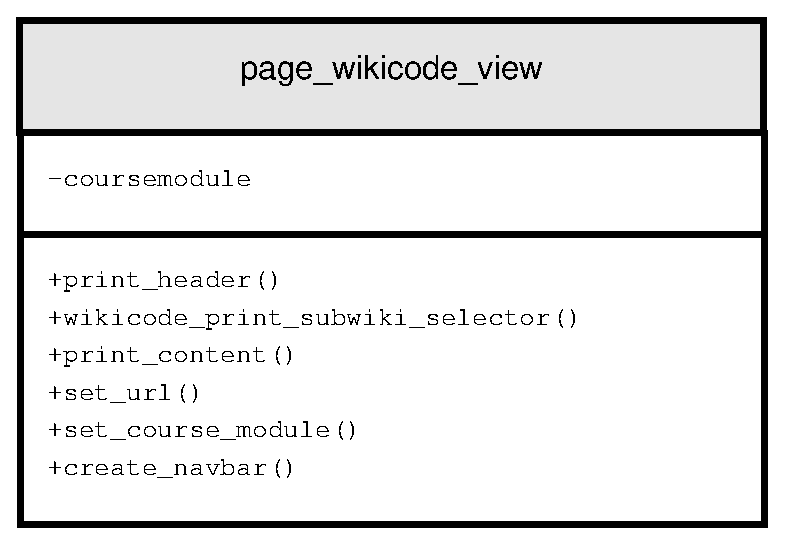
\includegraphics[width=0.5\textwidth]{./img/page_wikicode_view.eps}
			\caption{Class page\_wikicode\_view}
		\end{figure}
\end{itemize}

\subsubsection{Class page\_wikicode\_edit}

\begin{itemize}
	\item Descripción: Clase para mostrarnos una página de edición de Wikicode.
	\item Observaciones: Se considera que esta clase es la que hace de interfaz en los casos de uso \emph{Edición de código desarrollado}, \emph{Interacción mediante chat con otros usuarios} y \emph{Compilación de código fuente}.
	\item Atributos:
		\begin{itemize}
			\item compiled:
				\begin{itemize}
					\item Descripción: Variable que nos describe si la página actual se está mostrando tras una compilación o aún no se ha intentando compilar.
					\item Dominio: Variable de tipo entero.
				\end{itemize}
		\end{itemize}
	\item Operaciones:
		\begin{itemize}
			\item \textbf{print\_header: }Esta operación devuelve el código HTML que imprime la parte superior de la página.
			\item \textbf{print\_pagetitle: }Método para imprimir el título de la página.
			\item \textbf{print\_content: }Operación devuelve el código HTML que imprime la parte central de la página.
			\item \textbf{set\_url: }Operación que modifica las variables globales para indicar a Moodle en que página nos encontramos.
			\item \textbf{set\_session\_url: }Método para modificar la variable global de Moodle referente a la dirección web de la sesión.
			\item \textbf{set\_compiled: }Método para asignar la información referente a la variable compiled.
			\item \textbf{print\_edit: }Método que crea el código HTML que involucra al editor web, el chat y el compilador.
		\end{itemize}
	\item Relaciones:
		\begin{itemize}
			\item \textbf{page\_wikicode:} Hereda de esta clase.
			\item \textbf{page\_wikicode\_compile:} Padre de esta clase.
			\item \textbf{page\_wikicode\_save:} Padre de esta clase.
		\end{itemize}
	\item Diagrama de la clase:
		\begin{figure}[h]
			\centering
			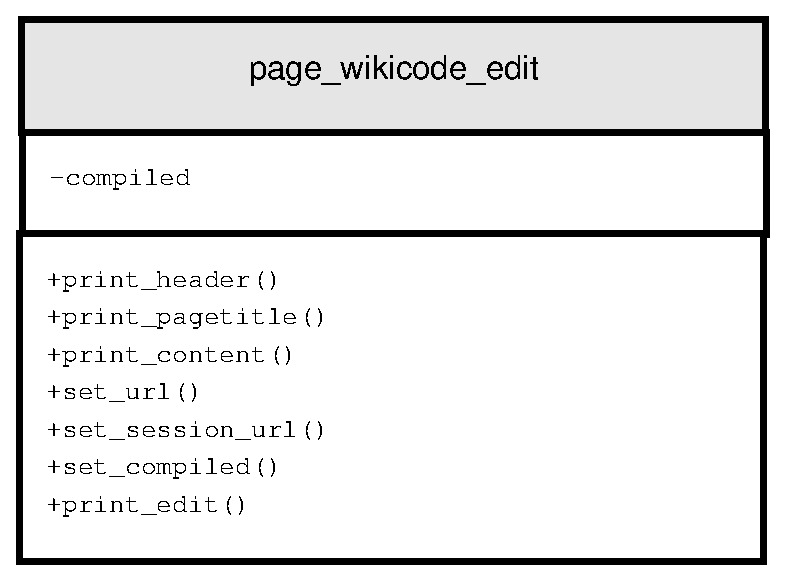
\includegraphics[width=0.5\textwidth]{./img/page_wikicode_edit.eps}
			\caption{Class page\_wikicode\_edit}
		\end{figure}
\end{itemize}

\subsubsection{Class page\_wikicode\_log}

\begin{itemize}
	\item Descripción: Clase para mostrarnos una página de estadísticas sobre una Wikicode.
	\item Observaciones: Se considera que esta clase es la que hace de interfaz con el caso de uso \emph{Consulta de estadísticas}.
	\item Atributos: No hay atributos.
	\item Operaciones:
		\begin{itemize}
			\item \textbf{print\_header: }Esta operación devuelve el código HTML que imprime la parte superior de la página.
			\item \textbf{print\_pagetitle: }Método para imprimir el título de la página.
			\item \textbf{print\_content: }Operación devuelve el código HTML que imprime la parte central de la página.
			\item \textbf{set\_url: }Operación que modifica las variables globales para indicar a Moodle en que página nos encontramos.
			\item \textbf{set\_session\_url: }Método para modificar la variable global de Moodle referente a la dirección web de la sesión.
			\item \textbf{print\_log: }Método que crea el código HTML que nos muestra las estadísticas de la página Wikicode actual.
		\end{itemize}
	\item Relaciones:
		\begin{itemize}
			\item \textbf{page\_wikicode:} Hereda de esta clase.
		\end{itemize}
	\item Diagrama de la clase:
		\begin{figure}[h]
			\centering
			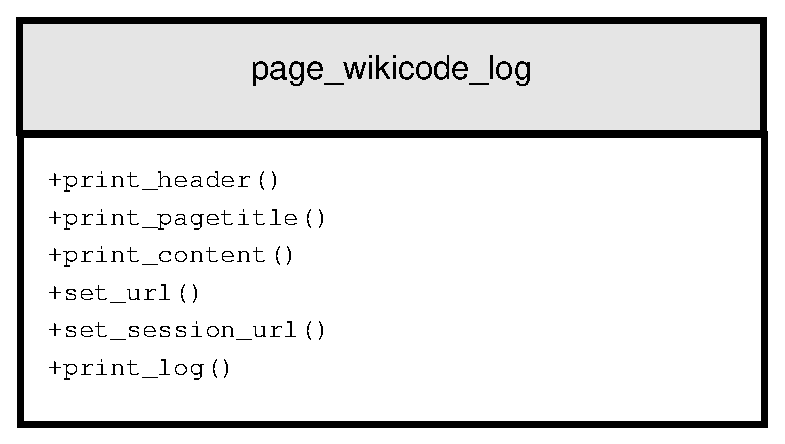
\includegraphics[width=0.5\textwidth]{./img/page_wikicode_log.eps}
			\caption{Class page\_wikicode\_log}
		\end{figure}
\end{itemize}

\subsubsection{Class page\_wikicode\_search}

\begin{itemize}
	\item Descripción: Clase para mostrarnos una búsqueda dentro de las páginas de Wikicode.
	\item Observaciones: Está clase sólo es utilizada a partir de la versión 2 de Moodle.
	\item Atributos:
		\begin{itemize}
			\item search\_result:
				\begin{itemize}
					\item Descripción: Variable que nos almacena un registro de base de datos con el resultado de la búsqueda que se desee.
					\item Dominio: Variable de tipo objeto.
				\end{itemize}
		\end{itemize}
	\item Operaciones:
		\begin{itemize}
			\item \textbf{create\_navbar: }Esta operación devuelve el código HTML de una barra de navegación.
			\item \textbf{set\_search\_string:} Función que llama a base de datos para conseguir los datos de la búsqueda. Recibe como parámetros la cadena a buscar y el dominio sobre el que se quiere encontrar la información.
			\item \textbf{print\_content: }Operación devuelve el código HTML que imprime la parte central de la página.
			\item \textbf{set\_url: }Operación que modifica las variables globales para indicar a Moodle en que página nos encontramos.
		\end{itemize}
	\item Relaciones:
		\begin{itemize}
			\item \textbf{page\_wikicode:} Hereda de esta clase.
		\end{itemize}
	\item Diagrama de la clase:
		\begin{figure}[h]
			\centering
			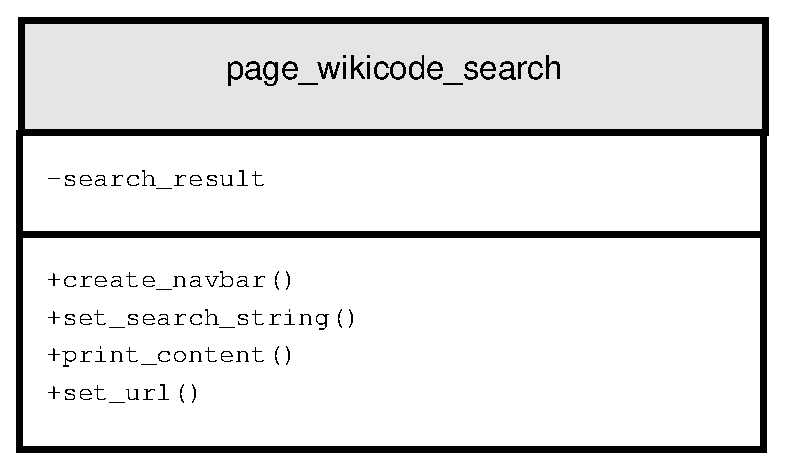
\includegraphics[width=0.5\textwidth]{./img/page_wikicode_search.eps}
			\caption{Class page\_wikicode\_search}
		\end{figure}
\end{itemize}

\subsubsection{Class page\_wikicode\_create}

\begin{itemize}
	\item Descripción: Clase para crear una nueva Wikicode dentro de un curso.
	\item Observaciones: Se considera que esta clase es la que hace de interfaz con el caso de uso \emph{Creación y Parametrización de la actividad Wikicode}.
	\item Atributos:
		\begin{itemize}
			\item format:
				\begin{itemize}
					\item Descripción: Formato de la Wikicode que se va a crear. Actualmente sólo existe uno, pero se deja el código preparada por si se desean crear más formatos en el futuro.
					\item Dominio: Variable de tipo string.
				\end{itemize}
			\item swid:
				\begin{itemize}
					\item Descripción: Identificador de la página subwiki seleccionada.
					\item Dominio: Variable de tipo entero.
				\end{itemize}
			\item wid:
				\begin{itemize}
					\item Descripción: Identificador de la página wiki seleccionada.
					\item Dominio: Variable de tipo entero.
				\end{itemize}
			\item action:
				\begin{itemize}
					\item Descripción: Cadena con la información sobre si se va a crear una página nueva o se está modificando una anterior.
					\item Dominio: Variable de tipo string.
				\end{itemize}
			\item mform:
				\begin{itemize}
					\item Descripción: Objeto con la información sobre la nueva página que se está creando.
					\item Dominio: Variable de tipo objeto.
				\end{itemize}
		\end{itemize}
	\item Operaciones:
		\begin{itemize}
			\item \textbf{print\_header: }Esta operación devuelve el código HTML que imprime la parte superior de la página.
			\item \textbf{print\_content: }Operación devuelve el código HTML que imprime la parte central de la página.
			\item \textbf{create\_navbar: }Esta operación devuelve el código HTML de una barra de navegación.
			\item \textbf{set\_url: }Operación que modifica las variables globales para indicar a Moodle en que página nos encontramos.
			\item \textbf{create\_page: }Método que crea el código HTML que nos muestra la página de parametrización de la Wikicode.
			\item \textbf{set\_format: }Método para asignar el formato de la Wikicode.
			\item \textbf{set\_wid: }Método para asignar el identificador de la Wikicode actual.
			\item \textbf{set\_swid: }Método para asignar el identificador de la subwiki actual.
			\item \textbf{set\_action: }Método para asignar la acción que se va a realizar.
		\end{itemize}
	\item Relaciones:
		\begin{itemize}
			\item \textbf{page\_wikicode:} Hereda de esta clase.
		\end{itemize}
	\item Diagrama de la clase:
		\begin{figure}[h]
			\centering
			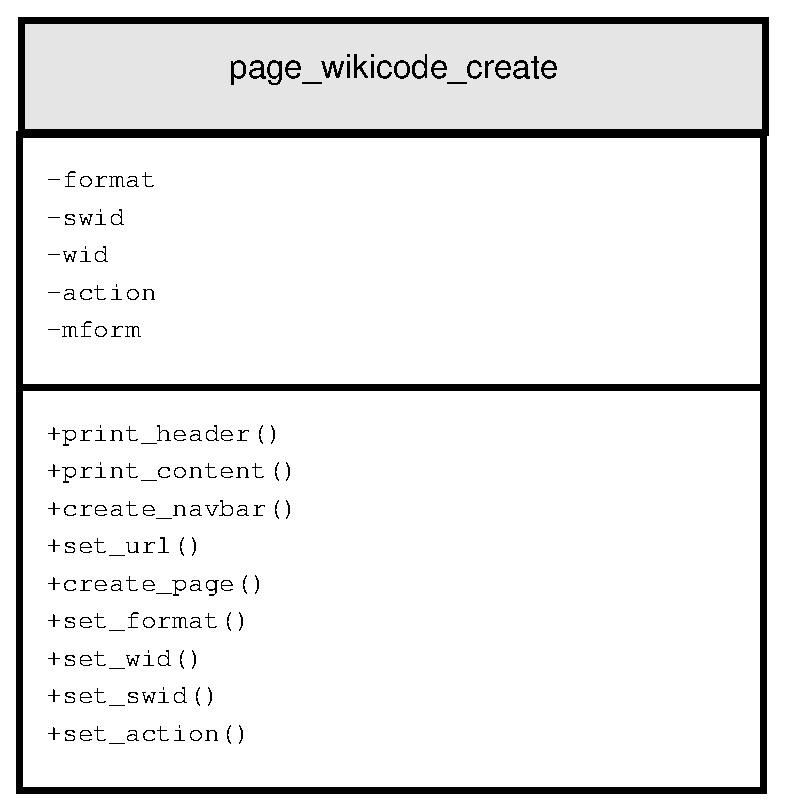
\includegraphics[width=0.5\textwidth]{./img/page_wikicode_create.eps}
			\caption{Class page\_wikicode\_create}
		\end{figure}
\end{itemize}

\subsubsection{Class page\_wikicode\_compile}

\begin{itemize}
	\item Descripción: Clase que llama al compilador y nos muestra el intercambio de información con éste.
	\item Observaciones: Se considera que esta clase es la que hace de interfaz entre el \emph{módulo Wikicode-Mod} y el compilador de C.
	\item Atributos:
		\begin{itemize}
			\item newcontent:
				\begin{itemize}
					\item Descripción: Código fuente sincronizado del editor que va a ser compilado.
					\item Dominio: Variable de tipo string.
				\end{itemize}
			\item download:
				\begin{itemize}
					\item Descripción: Identificador con la información sobre si se desea descargar el ejecutable en caso de que la compilación sea correcta.
					\item Dominio: Variable de tipo entero.
				\end{itemize}
		\end{itemize}
	\item Operaciones:
		\begin{itemize}
			\item \textbf{print\_header: }Esta operación devuelve el código HTML que imprime la parte superior de la página.
			\item \textbf{print\_content: }Operación devuelve el código HTML que imprime la parte central de la página.
			\item \textbf{set\_newcontent: }Operación que asigna el código fuente al atributo de la clase.
			\item \textbf{set\_download: }Método para asignar si se desea descargar el ejecutable.
			\item \textbf{print\_compile: }Operación de llamada al compilador y de recoger sus resultados. Para finalizar nos redirige a la página de edición con la nueva información.
		\end{itemize}
	\item Relaciones:
		\begin{itemize}
			\item \textbf{page\_wikicode\_edit:} Hereda de esta clase.
		\end{itemize}
	\item Diagrama de la clase:
		\begin{figure}[h]
			\centering
			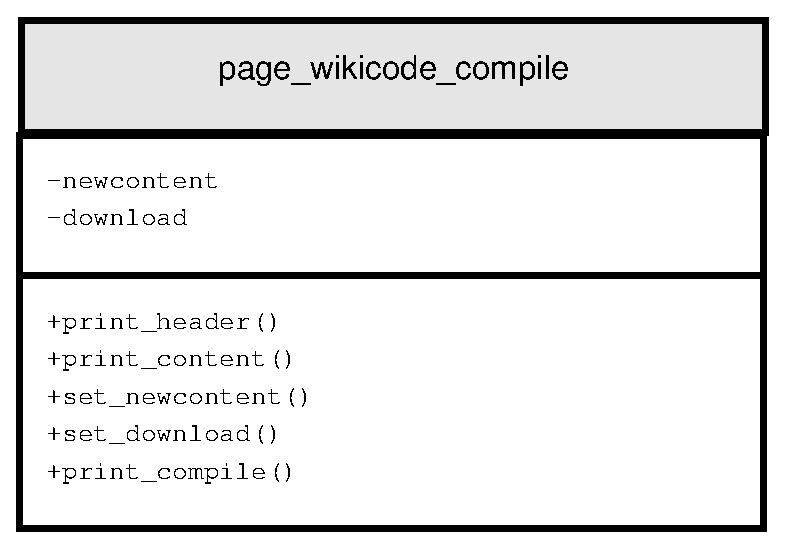
\includegraphics[width=0.5\textwidth]{./img/page_wikicode_compile.eps}
			\caption{Class page\_wikicode\_compile}
		\end{figure}
\end{itemize}

\subsubsection{Class page\_wikicode\_diff}

\begin{itemize}
	\item Descripción: Clase que nos muestra a través de un interfaz gráfico las diferencias entre dos versiones.
	\item Observaciones: Sólo disponible a partir de la versión 2 de Moodle.
	\item Atributos:
		\begin{itemize}
			\item compare:
				\begin{itemize}
					\item Descripción: Número de versión que quiere que se compare.
					\item Dominio: Variable de tipo entero.
				\end{itemize}
			\item comparewith:
				\begin{itemize}
					\item Descripción: Número de versión con el que se quiere comparar el atributo \emph{compare}.
					\item Dominio: Variable de tipo entero.
				\end{itemize}
		\end{itemize}
	\item Operaciones:
		\begin{itemize}
			\item \textbf{print\_header: }Esta operación devuelve el código HTML que imprime la parte superior de la página.
			\item \textbf{print\_content: }Operación devuelve el código HTML que imprime la parte central de la página.
			\item \textbf{set\_url: }Operación que modifica las variables globales para indicar a Moodle en que página nos encontramos.
			\item \textbf{set\_comparasion: }Operación que asigna las versiones que se quieren comparar.
			\item \textbf{print\_diff\_content: }Operación que compara ambas versiones, encuentra sus diferencias y nos devuelve el código HTML para mostrarlas con el interfaz de Moodle.
		\end{itemize}
	\item Relaciones:
		\begin{itemize}
			\item \textbf{page\_wikicode:} Hereda de esta clase.
		\end{itemize}
	\item Diagrama de la clase:
		\begin{figure}[h]
			\centering
			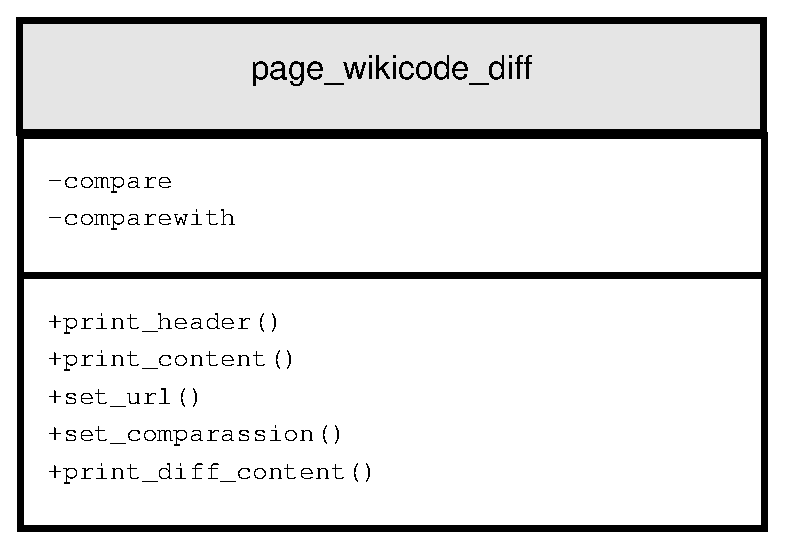
\includegraphics[width=0.5\textwidth]{./img/page_wikicode_diff.eps}
			\caption{Class page\_wikicode\_diff}
		\end{figure}
\end{itemize}

\subsubsection{Class page\_wikicode\_history}

\begin{itemize}
	\item Descripción: Clase que nos muestra el histórico de versiones de un módulo Wikicode.
	\item Observaciones: Se considera que esta clase es la que hace una parte de interfaz con el caso de uso \emph{Consulta de histórico y restauración de versiones}.
	\item Atributos:
		\begin{itemize}
			\item paging:
				\begin{itemize}
					\item Descripción: Versión actual.
					\item Dominio: Variable de tipo entero.
				\end{itemize}
			\item rowsperpage:
				\begin{itemize}
					\item Descripción: Versiones que se desean visualizar por página.
					\item Dominio: Variable de tipo entero.
				\end{itemize}
			\item allversion:
				\begin{itemize}
					\item Descripción: Si esta variable es distinta a 0, todas las versiones serán visualizadas en una tabla.
					\item Dominio: Variable de tipo entero.
				\end{itemize}
		\end{itemize}
	\item Operaciones:
		\begin{itemize}
			\item \textbf{print\_header: }Esta operación devuelve el código HTML que imprime la parte superior de la página.
			\item \textbf{print\_pagetitle: }Método para imprimir el título de la página.
			\item \textbf{print\_content: }Operación devuelve el código HTML que imprime la parte central de la página.
			\item \textbf{set\_url: }Operación que modifica las variables globales para indicar a Moodle en que página nos encontramos.
			\item \textbf{set\_paging: }Operación que asigna la versión actual sobre la que nos encontramos.
			\item \textbf{set\_allversion: }Operación que asigna si deseamos ver todas las versiones o un número limitado de estas.
			\item \textbf{print\_history\_content: }Operación que nos muestra el contenido de un histórico.
			\item \textbf{create\_navbar: }Esta operación devuelve el código HTML de una barra de navegación.
			\item \textbf{choose\_from\_radio:} Devuelve el código HTML tras crear un grupo de radiobutton con las opciones indicadas.
		\end{itemize}
	\item Relaciones:
		\begin{itemize}
			\item \textbf{page\_wikicode:} Hereda de esta clase.
		\end{itemize}
	\item Diagrama de la clase:
		\begin{figure}[h]
			\centering
			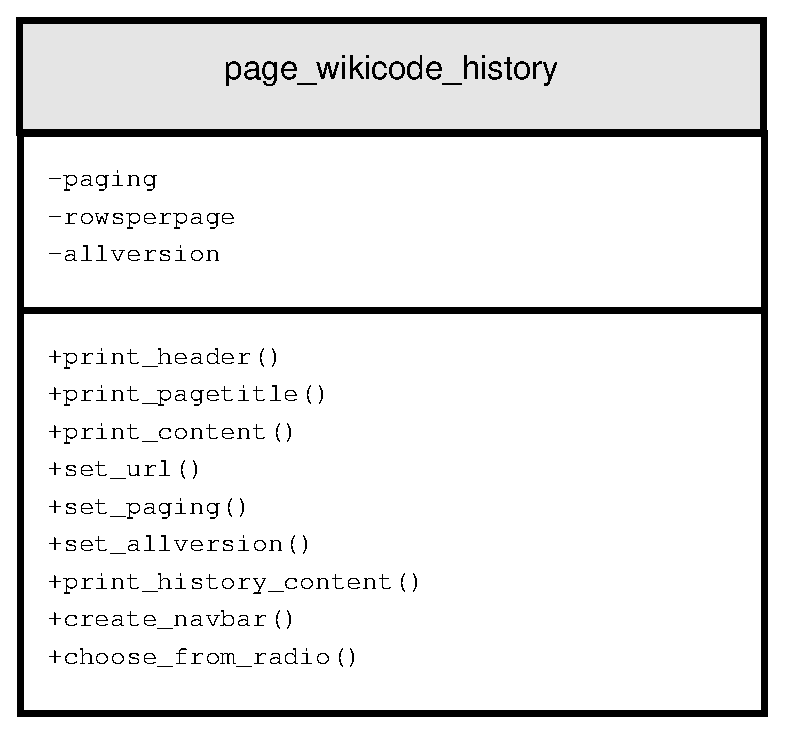
\includegraphics[width=0.5\textwidth]{./img/page_wikicode_history.eps}
			\caption{Class page\_wikicode\_history}
		\end{figure}
\end{itemize}

\subsubsection{Class page\_wikicode\_restoreversion}

\begin{itemize}
	\item Descripción: Clase que restaura una antigua versión de una Wikicode.
	\item Observaciones: Se considera que esta clase es la que hace una parte del interfaz con el caso de uso \emph{Consulta de histórico y restauración de versiones}.
	\item Atributos:
		\begin{itemize}
			\item version:
				\begin{itemize}
					\item Descripción: Identificador de versión que será restaurada.
					\item Dominio: Variable de tipo entero.
				\end{itemize}
		\end{itemize}
	\item Operaciones:
		\begin{itemize}
			\item \textbf{print\_header: }Esta operación devuelve el código HTML que imprime la parte superior de la página.
			\item \textbf{print\_content: }Operación devuelve el código HTML que imprime la parte central de la página.
			\item \textbf{set\_url: }Operación que modifica las variables globales para indicar a Moodle en que página nos encontramos.
			\item \textbf{set\_versionid: }Operación que asigna la versión que va a ser restaurada.
			\item \textbf{print\_restoreversion: }Imprime el contenido de la versión que se va a restaurar.
		\end{itemize}
	\item Relaciones:
		\begin{itemize}
			\item \textbf{page\_wikicode:} Hereda de esta clase.
		\end{itemize}
	\item Diagrama de la clase:
		\begin{figure}[h]
			\centering
			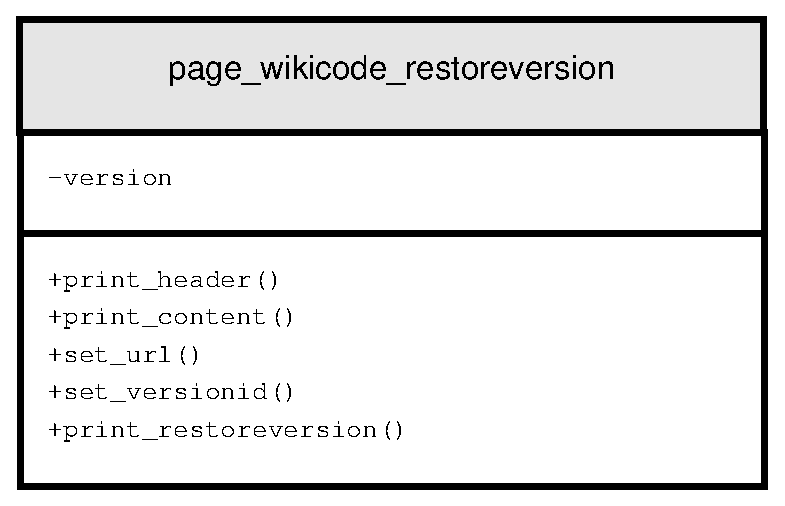
\includegraphics[width=0.5\textwidth]{./img/page_wikicode_restoreversion.eps}
			\caption{Class page\_wikicode\_restoreversion}
		\end{figure}
\end{itemize}

\subsubsection{Class page\_wikicode\_save}

\begin{itemize}
	\item Descripción: Clase que llama salva el código fuente en el histórico.
	\item Observaciones: Se considera que esta clase es la que hace de interfaz con el caso de uso \emph{Salvar Código}.
	\item Atributos:
		\begin{itemize}
			\item newcontent:
				\begin{itemize}
					\item Descripción: Código fuente sincronizado del editor que va a ser salvado.
					\item Dominio: Variable de tipo string.
				\end{itemize}
		\end{itemize}
	\item Operaciones:
		\begin{itemize}
			\item \textbf{print\_header: }Esta operación devuelve el código HTML que imprime la parte superior de la página.
			\item \textbf{print\_content: }Operación devuelve el código HTML que imprime la parte central de la página.
			\item \textbf{set\_newcontent: }Operación que asigna el código fuente al atributo de la clase.
			\item \textbf{print\_save: }Operación que salva en el histórico una nueva versión con el código fuente actual.
		\end{itemize}
	\item Relaciones:
		\begin{itemize}
			\item \textbf{page\_wikicode\_edit:} Hereda de esta clase.
			\item \textbf{page\_wikicode\_confirmrestore:} Padre de esta clase.
		\end{itemize}
	\item Diagrama de la clase:
		\begin{figure}[h]
			\centering
			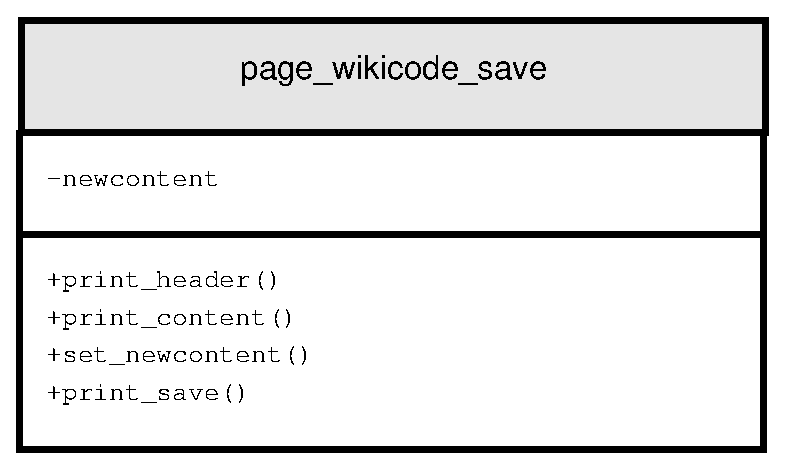
\includegraphics[width=0.5\textwidth]{./img/page_wikicode_save.eps}
			\caption{Class page\_wikicode\_save}
		\end{figure}
\end{itemize}

\subsubsection{Class page\_wikicode\_viewversion}

\begin{itemize}
	\item Descripción: Clase que nos muestra una antigua versión de una Wikicode.
	\item Observaciones: Se considera que esta clase es la que hace una parte del interfaz con el caso de uso \emph{Consulta de histórico y restauración de versiones}.
	\item Atributos:
		\begin{itemize}
			\item version:
				\begin{itemize}
					\item Descripción: Identificador de versión que será visualizada.
					\item Dominio: Variable de tipo entero.
				\end{itemize}
		\end{itemize}
	\item Operaciones:
		\begin{itemize}
			\item \textbf{print\_header: }Esta operación devuelve el código HTML que imprime la parte superior de la página.
			\item \textbf{print\_content: }Operación devuelve el código HTML que imprime la parte central de la página.
			\item \textbf{set\_url: }Operación que modifica las variables globales para indicar a Moodle en que página nos encontramos.
			\item \textbf{set\_versionid: }Operación que asigna la versión que va a ser restaurada.
			\item \textbf{print\_version\_view: }Imprime el contenido de una versión seleccionada.
		\end{itemize}
	\item Relaciones:
		\begin{itemize}
			\item \textbf{page\_wikicode:} Hereda de esta clase.
		\end{itemize}
	\item Diagrama de la clase:
		\begin{figure}[h]
			\centering
			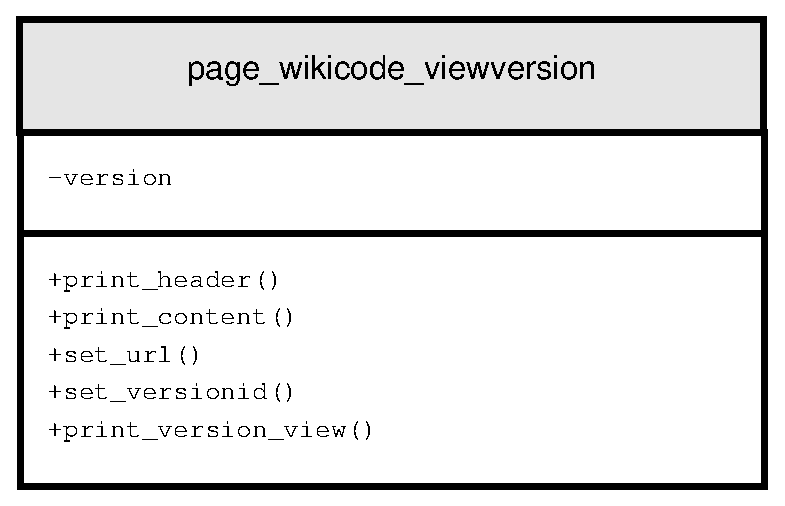
\includegraphics[width=0.5\textwidth]{./img/page_wikicode_viewversion.eps}
			\caption{Class page\_wikicode\_viewversion}
		\end{figure}
\end{itemize}

\subsubsection{Class page\_wikicode\_confirmrestore}

\begin{itemize}
	\item Descripción: Clase que nos pide confirmación sobre la restauración de una versión anterior y en caso de respuesta afirmativa la restaura.
	\item Observaciones: Se considera que esta clase es la que hace una parte del interfaz con el caso de uso \emph{Consulta de histórico y restauración de versiones}.
	\item Atributos:
		\begin{itemize}
			\item version:
				\begin{itemize}
					\item Descripción: Identificador de versión que será visualizada para la restauración.
					\item Dominio: Variable de tipo entero.
				\end{itemize}
		\end{itemize}
	\item Operaciones:
		\begin{itemize}
			\item \textbf{print\_content: }Operación devuelve el código HTML que imprime la parte central de la página.
			\item \textbf{set\_url: }Operación que modifica las variables globales para indicar a Moodle en que página nos encontramos.
			\item \textbf{set\_versionid: }Operación que asigna la versión que va a ser restaurada.
		\end{itemize}
	\item Relaciones:
		\begin{itemize}
			\item \textbf{page\_wikicode\_save:} Hereda de esta clase.
		\end{itemize}
	\item Diagrama de la clase:
		\begin{figure}[h]
			\centering
			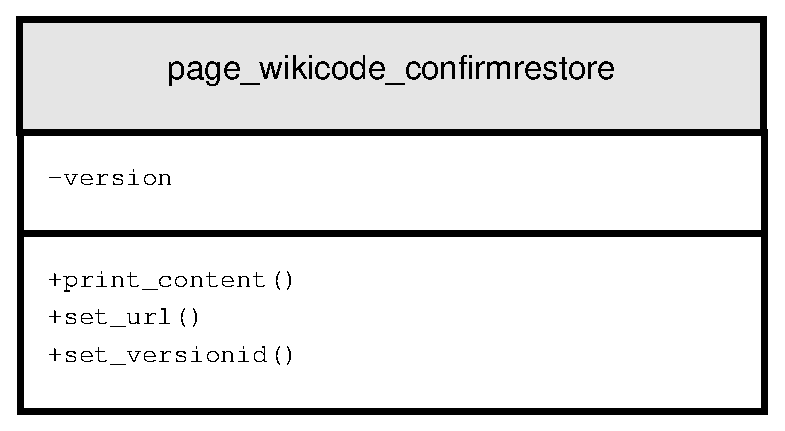
\includegraphics[width=0.5\textwidth]{./img/page_wikicode_confirmrestore.eps}
			\caption{Class page\_wikicode\_confirmrestore}
		\end{figure}
\end{itemize}

\subsubsection{Class page\_wikicode\_admin}

\begin{itemize}
	\item Descripción: Clase que nos muestra opciones de administración sobre nuestra Wikicode.
	\item Observaciones: Para visualizar la página ofrecida por esta clase es necesario tener rol de tutor en el curso.
	\item Atributos:
		\begin{itemize}
			\item action:
				\begin{itemize}
					\item Descripción: Información sobre la acción que va a realizar el administrador.
					\item Dominio: Variable de tipo string.
				\end{itemize}
		\end{itemize}
	\item Operaciones:
		\begin{itemize}
			\item \textbf{print\_header: }Esta operación devuelve el código HTML que imprime la parte superior de la página.
			\item \textbf{print\_content: }Operación que realiza la acción requerida por el administrador.
			\item \textbf{print\_delete\_content: }Operación que elimina el contenido de una Wikicode.
			\item \textbf{print\_delete\_version: }Operación que elimina una versión de Wikicode.
		\end{itemize}
	\item Relaciones:
		\begin{itemize}
			\item \textbf{page\_wikicode:} Hereda de esta clase.
		\end{itemize}
	\item Diagrama de la clase:
		\begin{figure}[h]
			\centering
			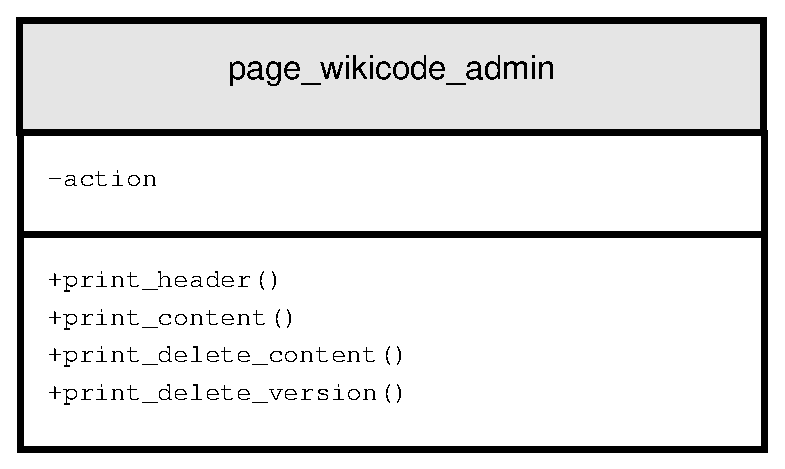
\includegraphics[width=0.5\textwidth]{./img/page_wikicode_admin.eps}
			\caption{Class page\_wikicode\_admin}
		\end{figure}
\end{itemize}

\subsubsection{Class html\_table}

\begin{itemize}
	\item Descripción: Clase que crea una tabla HTML.
	\item Observaciones: Esta clase sirve de esqueleto para diseñar una tabla HTML.
	\item Atributos:
		\begin{itemize}
			\item id:
				\begin{itemize}
					\item Descripción: Información sobre el atributo ID de la tabla.
					\item Dominio: Variable de tipo string.
				\end{itemize}
		\end{itemize}
		\begin{itemize}
			\item attributes:
				\begin{itemize}
					\item Descripción: Información sobre los atributos HTML de la tabla.
					\item Dominio: Variable de tipo array.
				\end{itemize}
		\end{itemize}
		\begin{itemize}
			\item head:
				\begin{itemize}
					\item Descripción: Objeto con información sobre la cabecera de la tabla.
					\item Dominio: Variable de tipo array.
				\end{itemize}
		\end{itemize}
		\begin{itemize}
			\item headspan:
				\begin{itemize}
					\item Descripción: Objeto con información sobre la cabecera de la tabla que puede ser utilizado para múltiples columnas.
					\item Dominio: Variable de tipo array.
				\end{itemize}
		\end{itemize}
		\begin{itemize}
			\item align:
				\begin{itemize}
					\item Descripción: Objeto con información sobre la alineación de la tabla.
					\item Dominio: Variable de tipo array.
				\end{itemize}
		\end{itemize}
		\begin{itemize}
			\item size:
				\begin{itemize}
					\item Descripción: Objeto con información sobre el tamaño de la tabla.
					\item Dominio: Variable de tipo array.
				\end{itemize}
		\end{itemize}
		\begin{itemize}
			\item wrap:
				\begin{itemize}
					\item Descripción: Información sobre la propiedad wrap de la tabla.
					\item Dominio: Variable de tipo array.
				\end{itemize}
		\end{itemize}
		\begin{itemize}
			\item data:
				\begin{itemize}
					\item Descripción: Información sobre los datos de la tabla.
					\item Dominio: Variable de tipo array.
				\end{itemize}
		\end{itemize}
		\begin{itemize}
			\item width:
				\begin{itemize}
					\item Descripción: Información sobre el tamaño de la tabla. Obsoleto a partir de la versión 2 de Moodle que utiliza hojas de estilo CSS.
					\item Dominio: Variable de tipo string.
				\end{itemize}
		\end{itemize}
		\begin{itemize}
			\item tablealign:
				\begin{itemize}
					\item Descripción:  Información sobre la alineación de la tabla. Obsoleto a partir de la versión 2 de Moodle que utiliza hojas de estilo CSS.
					\item Dominio: Variable de tipo string.
				\end{itemize}
		\end{itemize}
		\begin{itemize}
			\item cellpadding:
				\begin{itemize}
					\item Descripción:  Información sobre el margen de las celdas de la tabla. Obsoleto a partir de la versión 2 de Moodle que utiliza hojas de estilo CSS.
					\item Dominio: Variable de tipo entero.
				\end{itemize}
		\end{itemize}
		\begin{itemize}
			\item cellspacing:
				\begin{itemize}
					\item Descripción:  Información sobre el espacio entre celdas de la tabla. Obsoleto a partir de la versión 2 de Moodle que utiliza hojas de estilo CSS.
					\item Dominio: Variable de tipo entero.
				\end{itemize}
		\end{itemize}
		\begin{itemize}
			\item rowclasses:
				\begin{itemize}
					\item Descripción: Información sobre las clases a las que pertenece cada celda de la tabla.
					\item Dominio: Variable de tipo array.
				\end{itemize}
		\end{itemize}
		\begin{itemize}
			\item colclasses:
				\begin{itemize}
					\item Descripción: Información sobre las clases a las que pertenece cada columna de la tabla.
					\item Dominio: Variable de tipo array.
				\end{itemize}
		\end{itemize}
		\begin{itemize}
			\item summary:
				\begin{itemize}
					\item Descripción: Descripción de la tabla.
					\item Dominio: Variable de tipo string.
				\end{itemize}
		\end{itemize}
	\item Operaciones: -
	\item Relaciones: -
	\item Diagrama de la clase:
		\begin{figure}[h]
			\centering
			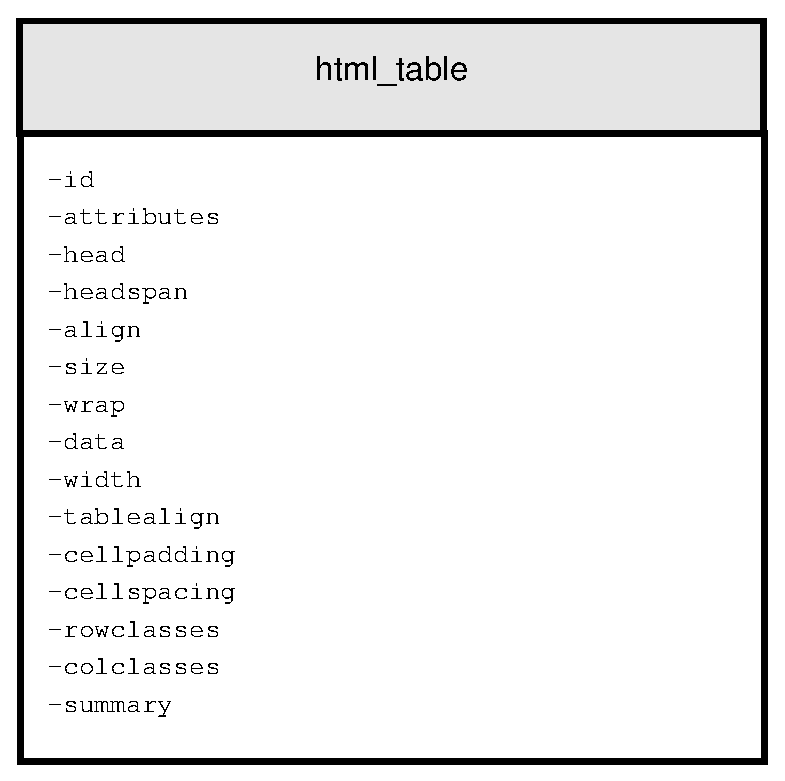
\includegraphics[width=0.5\textwidth]{./img/html_table.eps}
			\caption{Class html\_table}
		\end{figure}
\end{itemize}

\subsubsection{Class html\_write}

\begin{itemize}
	\item Descripción: Clase que nos devuelve el código HTML de distintos objetos web.
	\item Observaciones: Esta clase está disponible en el propio Moodle a partir de la versión 2, sin embargo se ha adaptado parcialmente y distribuido para la versión 1 de Moodle.
	\item Atributos: -
	\item Operaciones:
		\begin{itemize}
			\item \textbf{tag:} Devuelve el código HTML de un campo tipo tag.
			\item \textbf{start\_tag:} Devuelve la apertura del código HTML de un campo tipo tag.
			\item \textbf{end\_tag:} Devuelve el cerrado del código HTML de un campo tipo tag.
			\item \textbf{checkbox:} Devuelve el código HTML de un campo tipo checkbox.
			\item \textbf{table:} Devuelve el código HTML renderizado de un campo tipo table. Hace uso de la clase \emph{html\_table} como parámetro de entrada.
			\item \textbf{label:} Devuelve el código HTML de un campo tipo label.
		\end{itemize}
	\item Relaciones: -
	\item Diagrama de la clase:
		\begin{figure}[h]
			\centering
			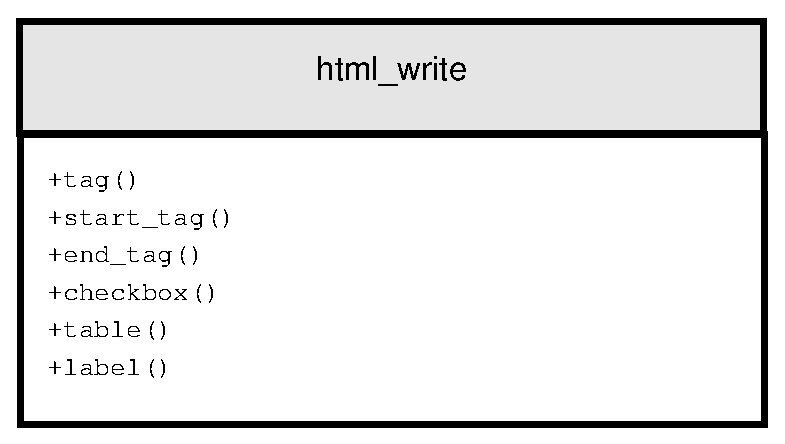
\includegraphics[width=0.5\textwidth]{./img/html_write.eps}
			\caption{Class html\_write}
		\end{figure}
\end{itemize}

\subsubsection{Class html\_table\_cell}

\begin{itemize}
	\item Descripción: Clase que define una celda de una tabla HTML.
	\item Observaciones: Esta clase está disponible en el propio Moodle a partir de la versión 2, sin embargo se ha adaptado parcialmente y distribuido para la versión 1 de Moodle.
	\item Atributos:
		\begin{itemize}
			\item id:
				\begin{itemize}
					\item Descripción: Información sobre el atributo ID de la celda.
					\item Dominio: Variable de tipo string.
				\end{itemize}
		\end{itemize}
		\begin{itemize}
			\item text:
				\begin{itemize}
					\item Descripción: Información sobre el contenido de la celda.
					\item Dominio: Variable de tipo string.
				\end{itemize}
		\end{itemize}
		\begin{itemize}
			\item abbr:
				\begin{itemize}
					\item Descripción: Información sobre el contenido abreviado de la celda.
					\item Dominio: Variable de tipo string.
				\end{itemize}
		\end{itemize}
		\begin{itemize}
			\item colspan:
				\begin{itemize}
					\item Descripción: Información sobre el número de columnas de la celda.
					\item Dominio: Variable de tipo string.
				\end{itemize}
		\end{itemize}
		\begin{itemize}
			\item rowspan:
				\begin{itemize}
					\item Descripción: Información sobre el número de filas de la celda.
					\item Dominio: Variable de tipo string.
				\end{itemize}
		\end{itemize}
		\begin{itemize}
			\item scope:
				\begin{itemize}
					\item Descripción: Define la forma de asociar la cabecera de las celdas y sus datos en una tabla.
					\item Dominio: Variable de tipo string.
				\end{itemize}
		\end{itemize}
		\begin{itemize}
			\item header:
				\begin{itemize}
					\item Descripción: Información sobre si tiene cabecera la celda.
					\item Dominio: Variable de tipo booleana.
				\end{itemize}
		\end{itemize}
		\begin{itemize}
			\item style:
				\begin{itemize}
					\item Descripción: Información sobre el contenido del atributo valor style de la celda.
					\item Dominio: Variable de tipo string.
				\end{itemize}
		\end{itemize}
		\begin{itemize}
			\item attributes:
				\begin{itemize}
					\item Descripción: Información sobre el contenido de otros atributos de la celda.
					\item Dominio: Variable de tipo objeto.
				\end{itemize}
		\end{itemize}
	\item Operaciones: -
	\item Relaciones: Esta clase está únicamente creada para que pueda ser utilizada por la clase html\_row.
	\newpage
	\item Diagrama de la clase:
		\begin{figure}[h]
			\centering
			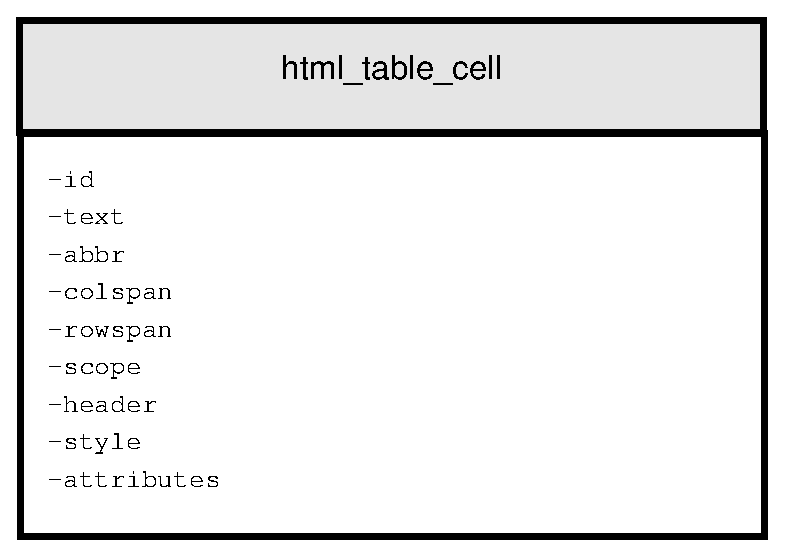
\includegraphics[width=0.5\textwidth]{./img/html_table_cell.eps}
			\caption{Class html\_cell}
		\end{figure}
\end{itemize}

\subsubsection{Class html\_table\_row}

\begin{itemize}
	\item Descripción: Clase que define una fila de una tabla HTML.
	\item Observaciones: Esta clase está disponible en el propio Moodle a partir de la versión 2, sin embargo se ha adaptado parcialmente y distribuido para la versión 1 de Moodle.
	\item Atributos:
		\begin{itemize}
			\item id:
				\begin{itemize}
					\item Descripción: Información sobre el atributo ID de la celda.
					\item Dominio: Variable de tipo string.
				\end{itemize}
		\end{itemize}
		\begin{itemize}
			\item cells:
				\begin{itemize}
					\item Descripción: Vector con información sobre las celdas de la fila.
					\item Dominio: Variable de tipo objeto.
				\end{itemize}
		\end{itemize}
		\begin{itemize}
			\item style:
				\begin{itemize}
					\item Descripción: Información sobre el contenido del atributo valor style de la celda.
					\item Dominio: Variable de tipo string.
				\end{itemize}
		\end{itemize}
		\begin{itemize}
			\item attributes:
				\begin{itemize}
					\item Descripción: Información sobre el contenido de otros atributos de la celda.
					\item Dominio: Variable de tipo objeto.
				\end{itemize}
		\end{itemize}
	\item Operaciones: -
	\item Relaciones: Esta clase está únicamente creada para que pueda ser utilizada por la clase html\_table.
	\item Diagrama de la clase:
		\begin{figure}[h]
			\centering
			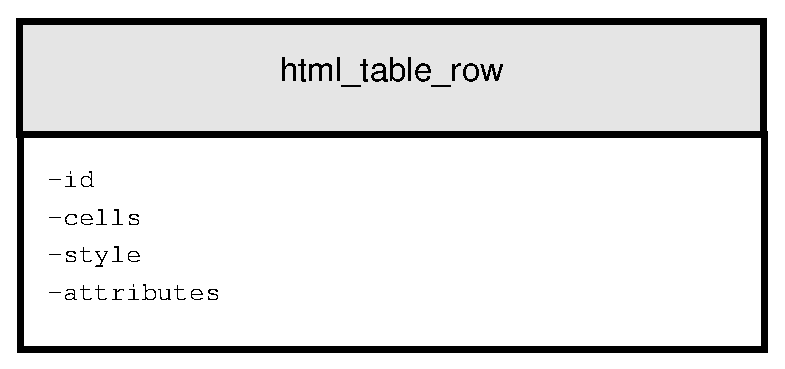
\includegraphics[width=0.5\textwidth]{./img/html_table_row.eps}
			\caption{Class html\_row}
		\end{figure}
\end{itemize}

\subsection{Diccionario de datos para el sistema Wikicode-Synchronizer}

Todas las funcionalidades de este subsistema han sido integrados en una única clase almacenada en un fichero PHP. Su descripción es la siguiente:

\subsubsection{Class editorlib}

\begin{itemize}
	\item Descripción: Clase que hace de interfaz entre el módulo de Moodle y los datos para su sincronización.
	\item Observaciones: Esta clase puede ser exportada para trabajar bajo otro sistema e-learning.
	\item Atributos:
		\begin{itemize}
			\item editorCode:
				\begin{itemize}
					\item Descripción: Código fuente que se quiere sincronizar.
					\item Dominio: Variable de tipo string.
				\end{itemize}
		\end{itemize}
		\begin{itemize}
			\item position:
				\begin{itemize}
					\item Descripción: Información sobre la posición de la tecla que ha sido pulsada para llamar al sincronizador.
					\item Dominio: Variable de tipo entero.
				\end{itemize}
		\end{itemize}
		\begin{itemize}
			\item pageid:
				\begin{itemize}
					\item Descripción: Información del identificador del código fuente.
					\item Dominio: Variable de tipo entero.
				\end{itemize}
		\end{itemize}
		\begin{itemize}
			\item del:
				\begin{itemize}
					\item Descripción: Información sobre si la operación realizada en el editor es de borrado.
					\item Dominio: Variable de tipo booleana.
				\end{itemize}
		\end{itemize}
		\begin{itemize}
			\item char\_del:
				\begin{itemize}
					\item Descripción: Código decimal del carácter que ha sido eliminado del código fuente.
					\item Dominio: Variable de tipo entero.
				\end{itemize}
		\end{itemize}
	\item Operaciones:
		\begin{itemize}
			\item \textbf{deleteEnterRepeat:} Elimina la aparición de varios saltos de línea repetidos.
			\item \textbf{getFunction:} Devuelve el nombre de la función al que pertenece una determinada posición dentro de un código fuente.
			\item \textbf{getLevel:} Devuelve el nivel de indexación en una determinada posición de un cursor dentro de un código fuente.
			\item \textbf{isLocked:} Información sobre si una determinada función está bloqueada dentro de un código fuente.
			\item \textbf{isLockedByUser:} Información sobre si una determinada función está bloqueada dentro de un código fuente por el usuario que hace la llamada al sincroonizador.
			\item \textbf{lockFunction:} Operación que bloquea una determinada función dentro de un código fuente.
			\item \textbf{unlockFunction:} Operación que desbloquea una determinada función dentro de un código fuente.
			\item \textbf{getLocksByUser:} Operación que devuelve el nombre de las funciones que tiene bloqueada un usuario dentro de un código fuente.
			\item \textbf{getInitFunctionLock:} Operación que devuelve la posición inicial del bloqueo de una función dentro de un código fuente.
			\item \textbf{getEndFunctionLock:} Operación que devuelve la posición final del bloqueo de una función dentro de un código fuente.
			\item \textbf{getFunctionLock:} Operación que devuelve una cadena con la función bloqueada delimitada por sus tags.
			\item \textbf{changeFunctionLock:} Operación que modifica una función bloqueada por otra dentro de un determinado código fuente.
			\item \textbf{getCodigoFromDB:} Operación que devuelve el código fuente almacenado en base de datos.
			\item \textbf{saveCodigoToDB:} Operación que salva el código fuente a la base de datos.
			\item \textbf{keypress:} Trigger lanzado cuando una tecla clave es pulsada en el editor asociado.
			\item \textbf{removePairKey:} Trigger lanzado cuando el usuario intenta eliminar una parte necesaria del código.
			\item \textbf{unlockFunctionDB:} Procedimiento lanzado cuando un usuario quiere desbloquear una serie de funciones que tiene bloqueada.		
		\end{itemize}
	\item Relaciones: -
	\item Diagrama de la clase:
		\begin{figure}[h]
			\centering
			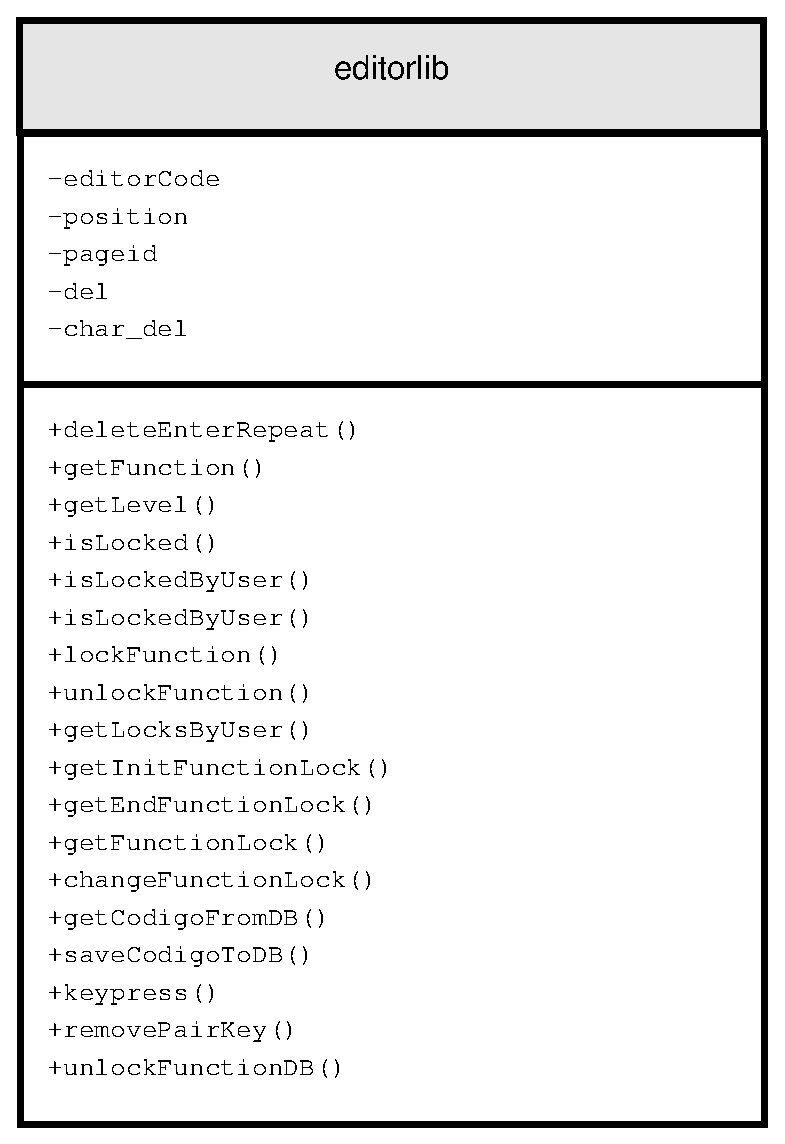
\includegraphics[width=0.5\textwidth]{./img/editorlib.eps}
			\caption{Class editorlib}
		\end{figure}
\end{itemize}

\newpage

\subsection{Diagrama de clases}

El diagrama de clases es el siguiente:

\begin{figure}[h]
	\centering
	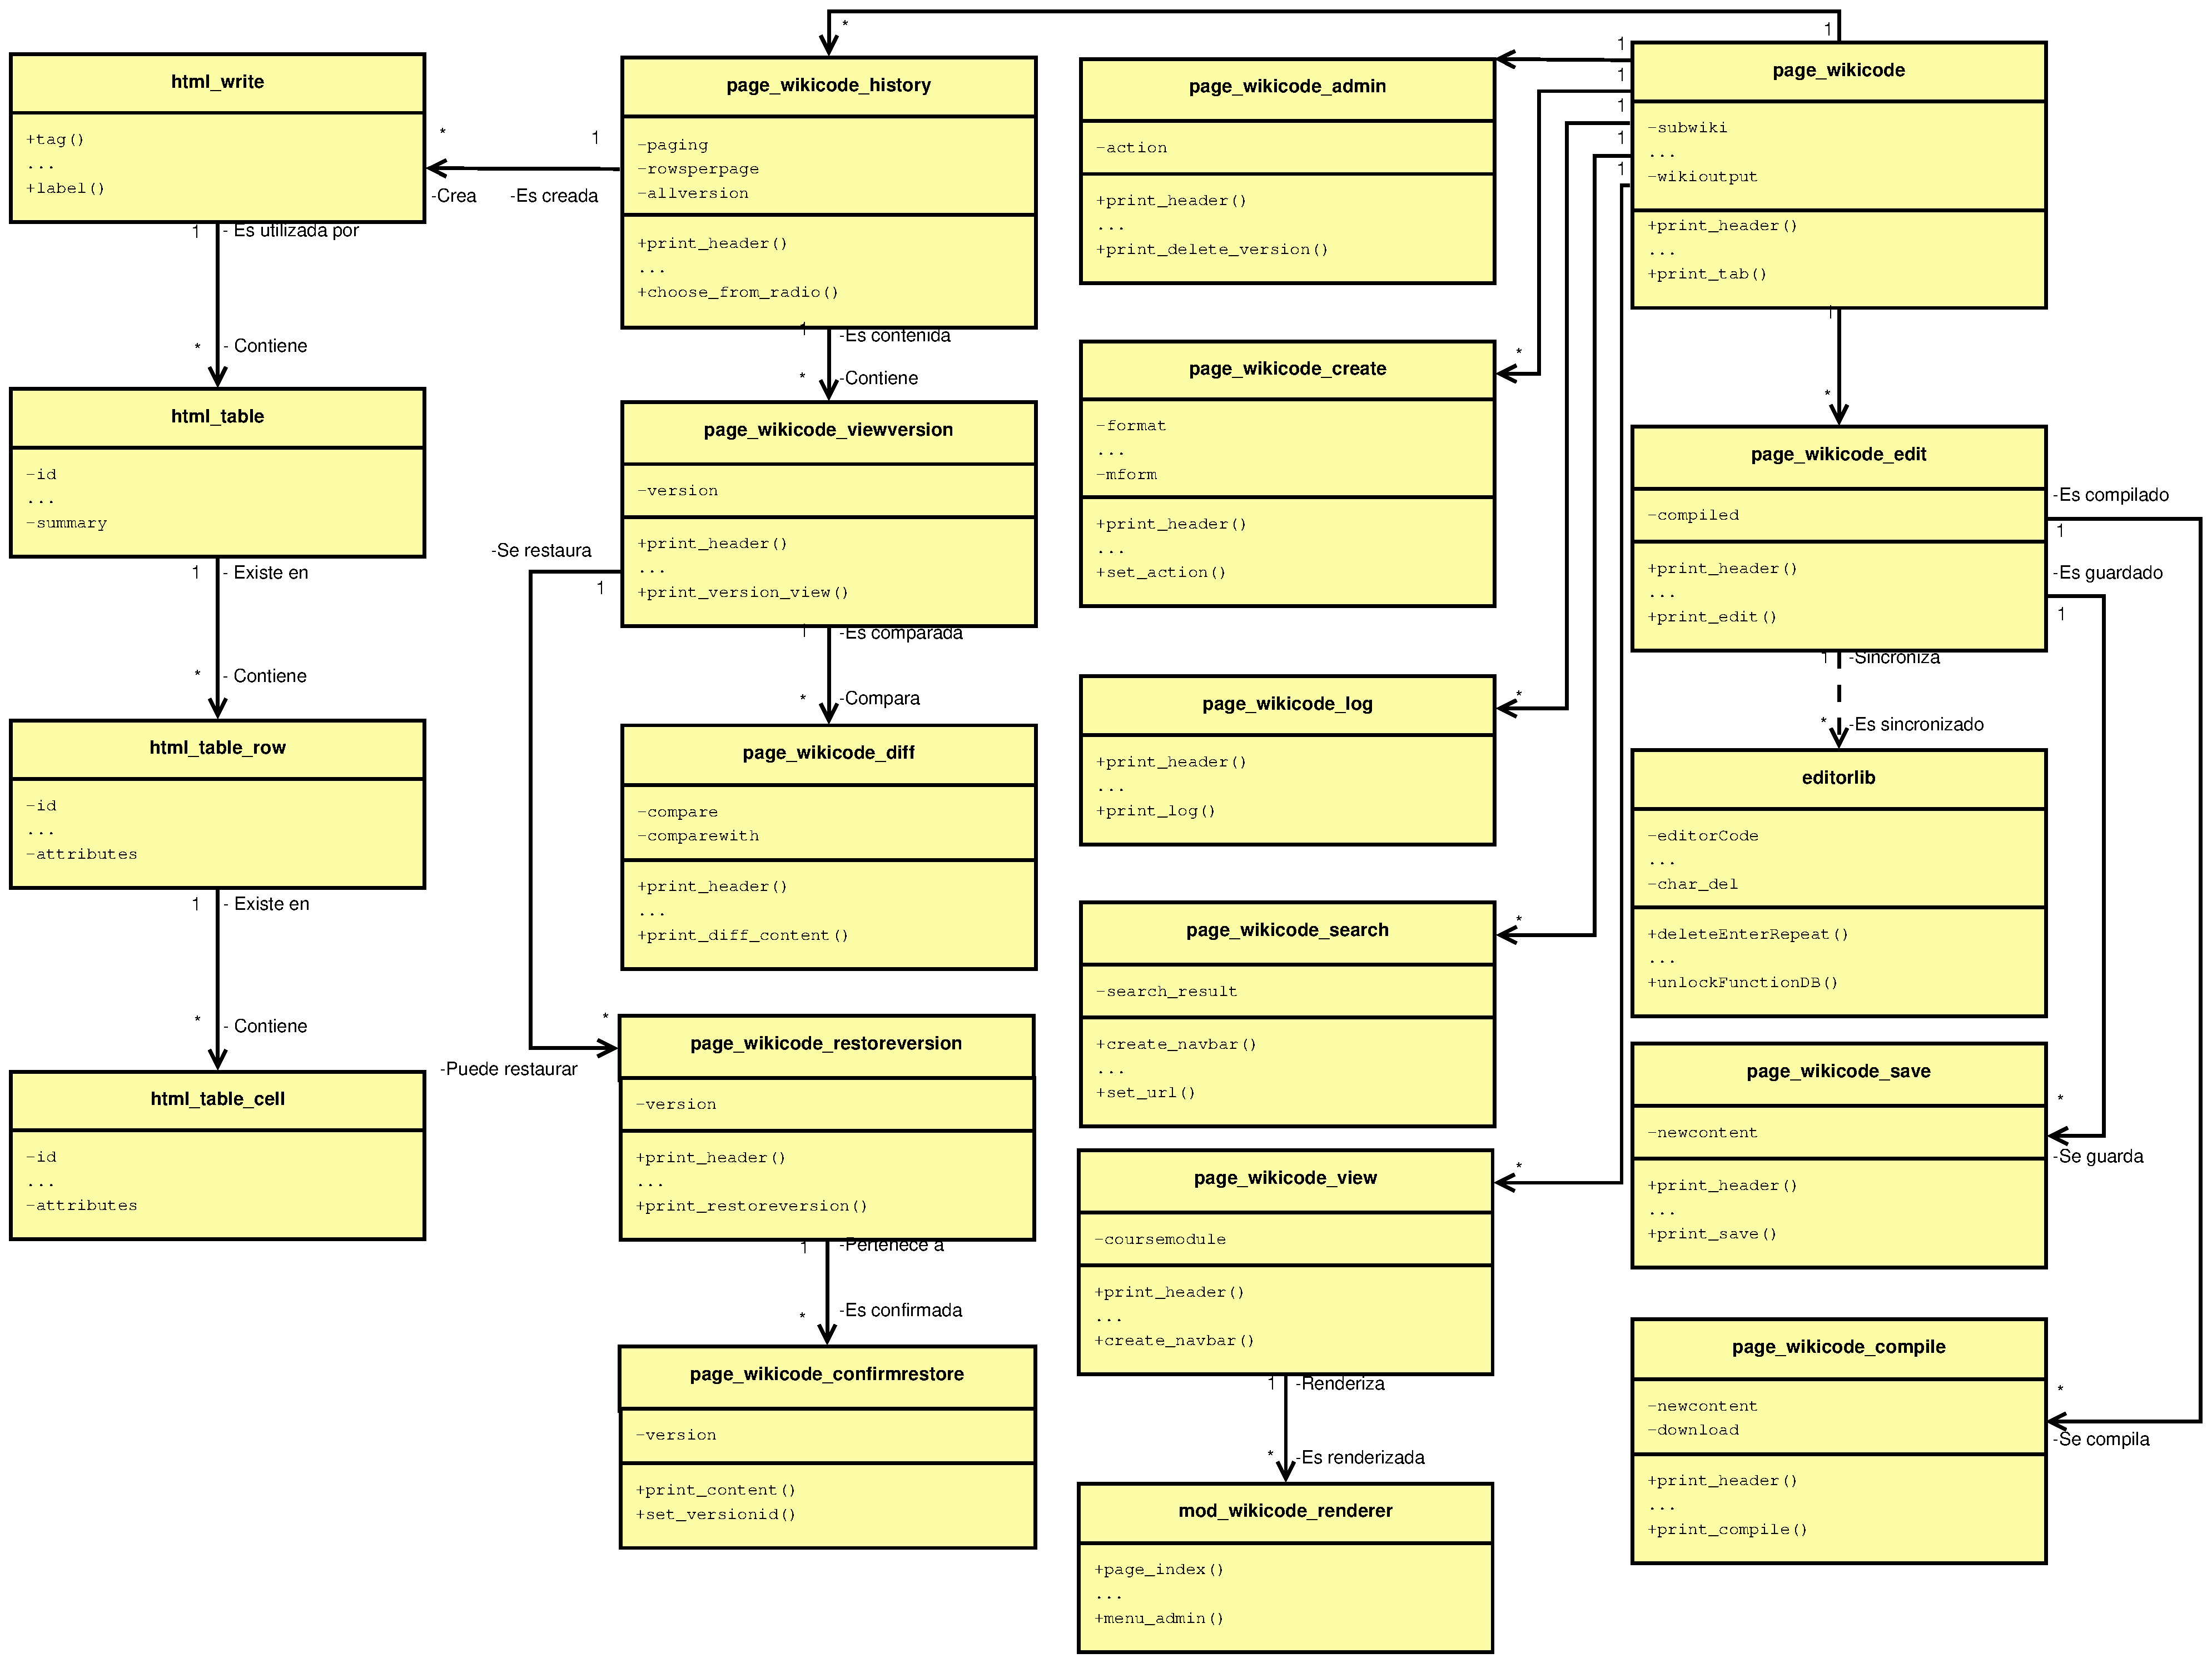
\includegraphics[width=1.1\textwidth]{./img/DiagramaCLASES.eps}
	\caption{Diagrama de clases}
\end{figure}

\newpage

\section{Especificación del Modelo Objeto-Comportamiento}

Una vez representados los elementos estáticos del sistema ahora es el momento de hacer una transición a su comportamiento dinámico. El aspecto dinámico del sistema combina la parte estructural con la dimensión del tiempo.

El modelo objeto-comportamiento representa cómo interaccionan las clases, especificando un flujo de control (secuencia de mensajes entre objetos) a lo largo del tiempo, para la ejecución de una tarea.

UML (\emph{Unified Modeling Language}) 2.0 proporciona dos tipos de diagramas de interacción: los diagramas de secuencia y los diagramas de colaboración. Se ha decidido usar diagramas de colaboración porque en ellos se destaca la organización estructural de los objetos que envían y reciben mensajes. En los apartados siguientes se desarrollan los diagramas de interacción más significativos dentro de la funcionalidad requerida.

\subsection{Diagrama de colaboración: Configuración de la Wikicode}

En este diagrama se pretende mostrar el flujo de eventos relacionado con la configuración de una nueva Wikicode.

Flujo de sucesos:

\begin{enumerate}
	\item Envía la configuración de parámetros.
	\item Confirma que la configuración es válida.
\end{enumerate}

\begin{figure}[h]
	\centering
	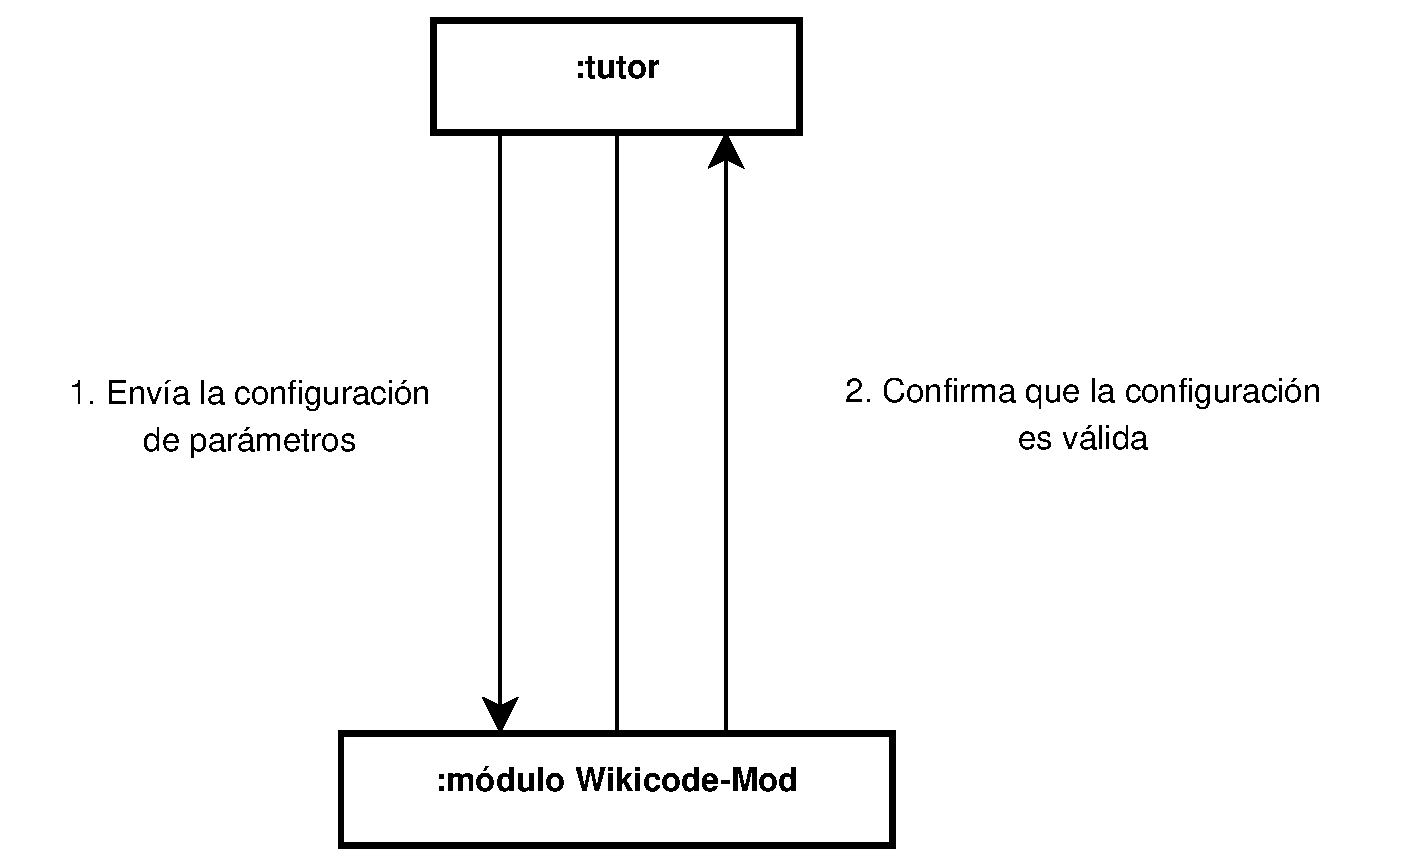
\includegraphics[width=0.5\textwidth]{./img/c3-dia-col1.eps}
	\caption{Diagrama de colaboración Configuración de la Wikicode}
\end{figure}

\subsection{Diagrama de colaboración: Visualización del Código Fuente}

En este diagrama se pretende mostrar el flujo de eventos relacionado con la visualización del código fuente dentro de Wikicode.

Flujo de sucesos:

\begin{enumerate}
	\item Solicita la visualización del código fuente.
	\item Se muestra el código.
\end{enumerate}

\begin{figure}[h]
	\centering
	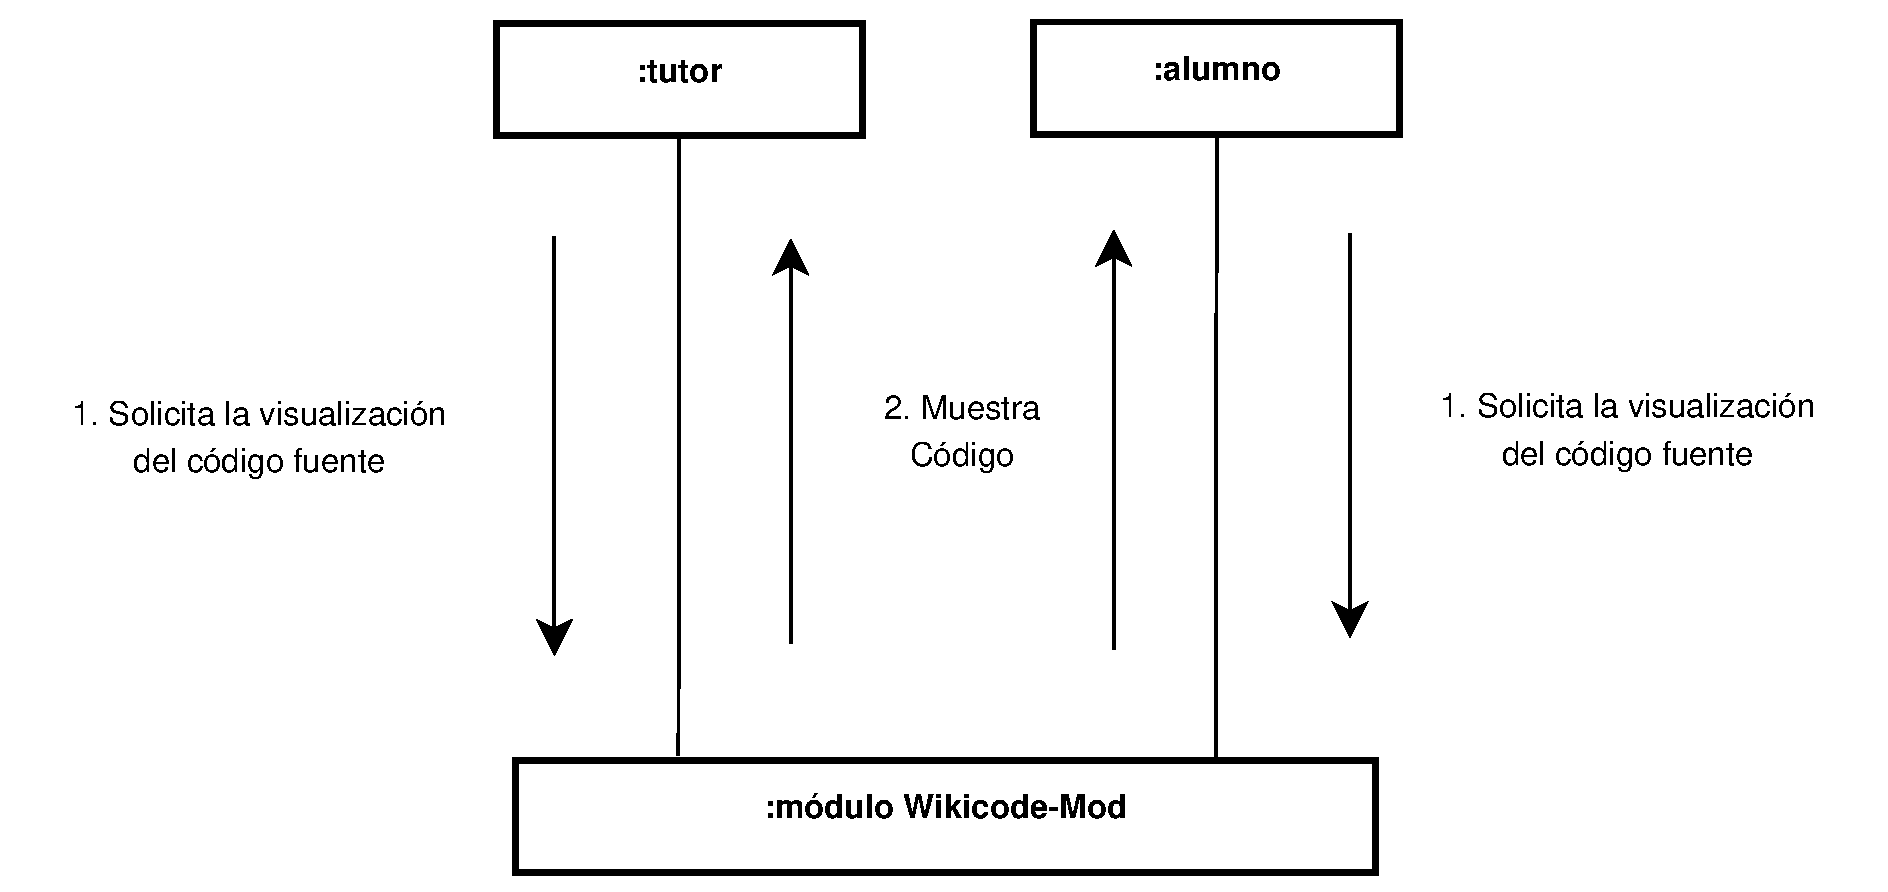
\includegraphics[width=0.5\textwidth]{./img/c3-dia-col2.eps}
	\caption{Diagrama de colaboración Visualización del Código Fuente}
\end{figure}

\newpage

\subsection{Diagrama de colaboración: Compilación de Código Fuente}

En este diagrama se pretende mostrar el flujo de eventos relacionado con la compilación de código fuente dentro de Wikicode.

Flujo de sucesos:

\begin{enumerate}
	\item Solicita la compilación del código fuente.
	\item Creación de los ficheros necesarios y petición de compilación al compilador.
	\item Se recoge la información de la compilación y se almacena.
	\item Se envía la información sobre la compilación.
	\item Se muestra la información sobre la compilación.
\end{enumerate}

\begin{figure}[h]
	\centering
	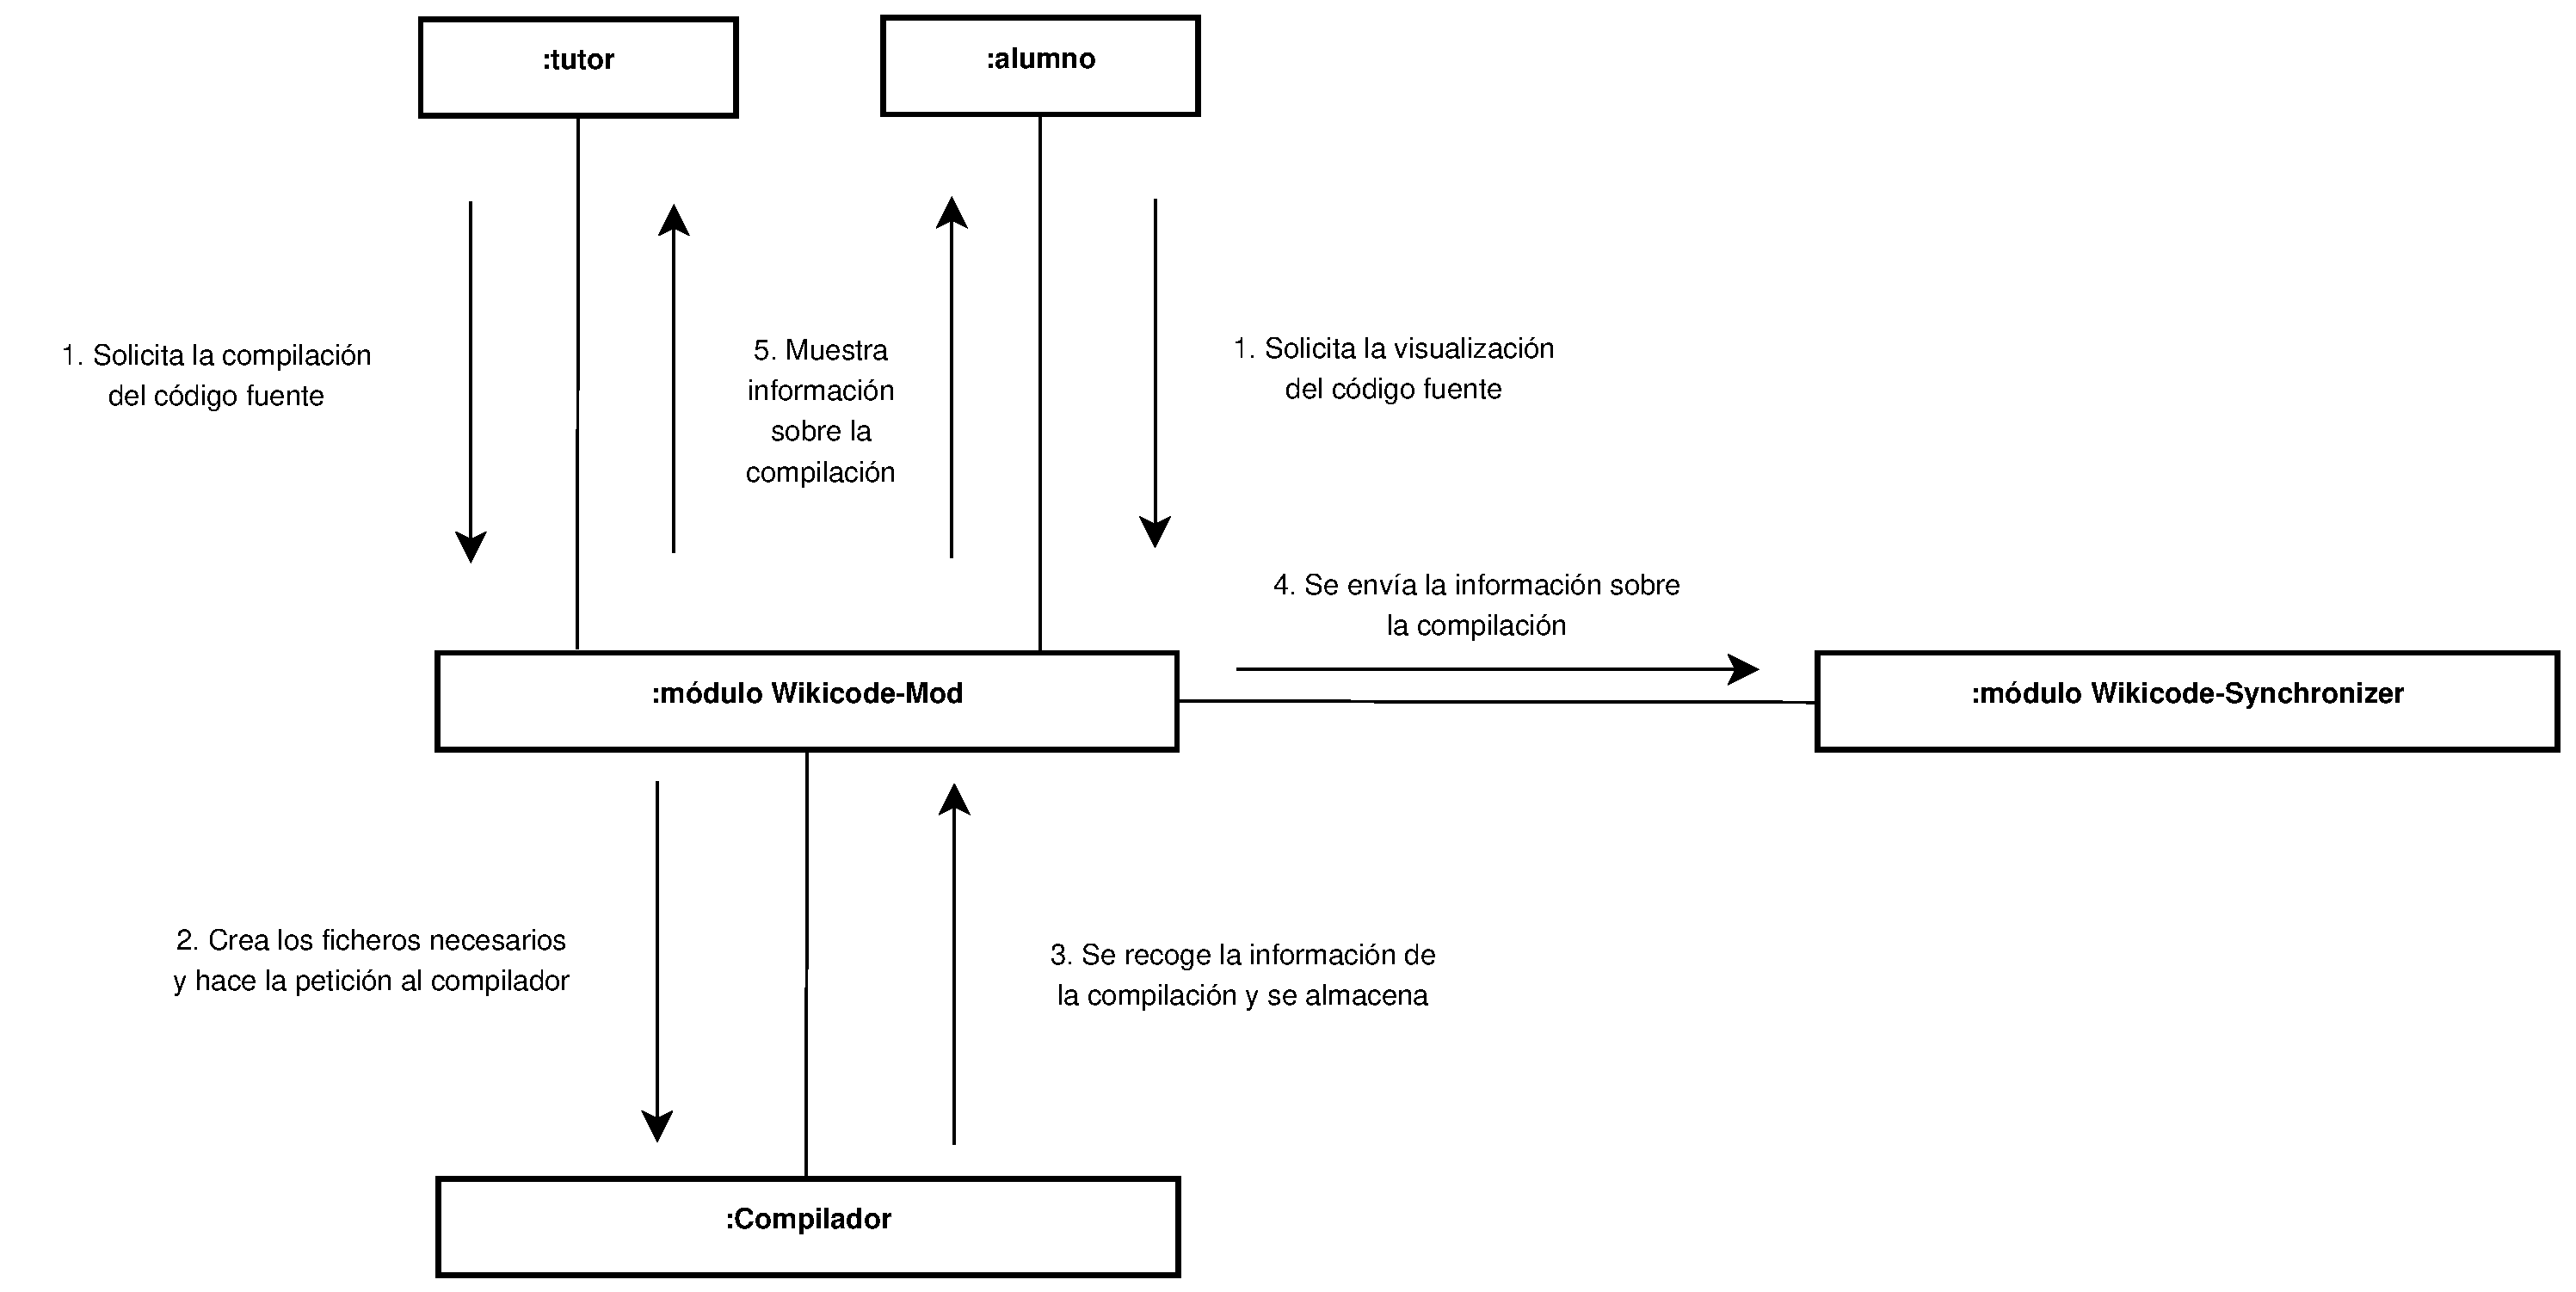
\includegraphics[width=\textwidth]{./img/c3-dia-col3.eps}
	\caption{Diagrama de colaboración Compilación de Código Fuente}
\end{figure}

\subsection{Diagrama de colaboración: Edición de código}

En este diagrama se pretende mostrar el flujo de eventos relacionado con la edición de código dentro de Wikicode.

Flujo de sucesos:

\begin{enumerate}
	\item Se edita el código y se pulsa una tecla clave.
	\item Se envía el nuevo código y la posición del carácter que ha sido modificado.
	\item Se sincroniza el código, se almacena en base de datos y se envía el nuevo código fuente.
	\item Se muestra el nuevo código sincronizado.
\end{enumerate}

\begin{figure}[h]
	\centering
	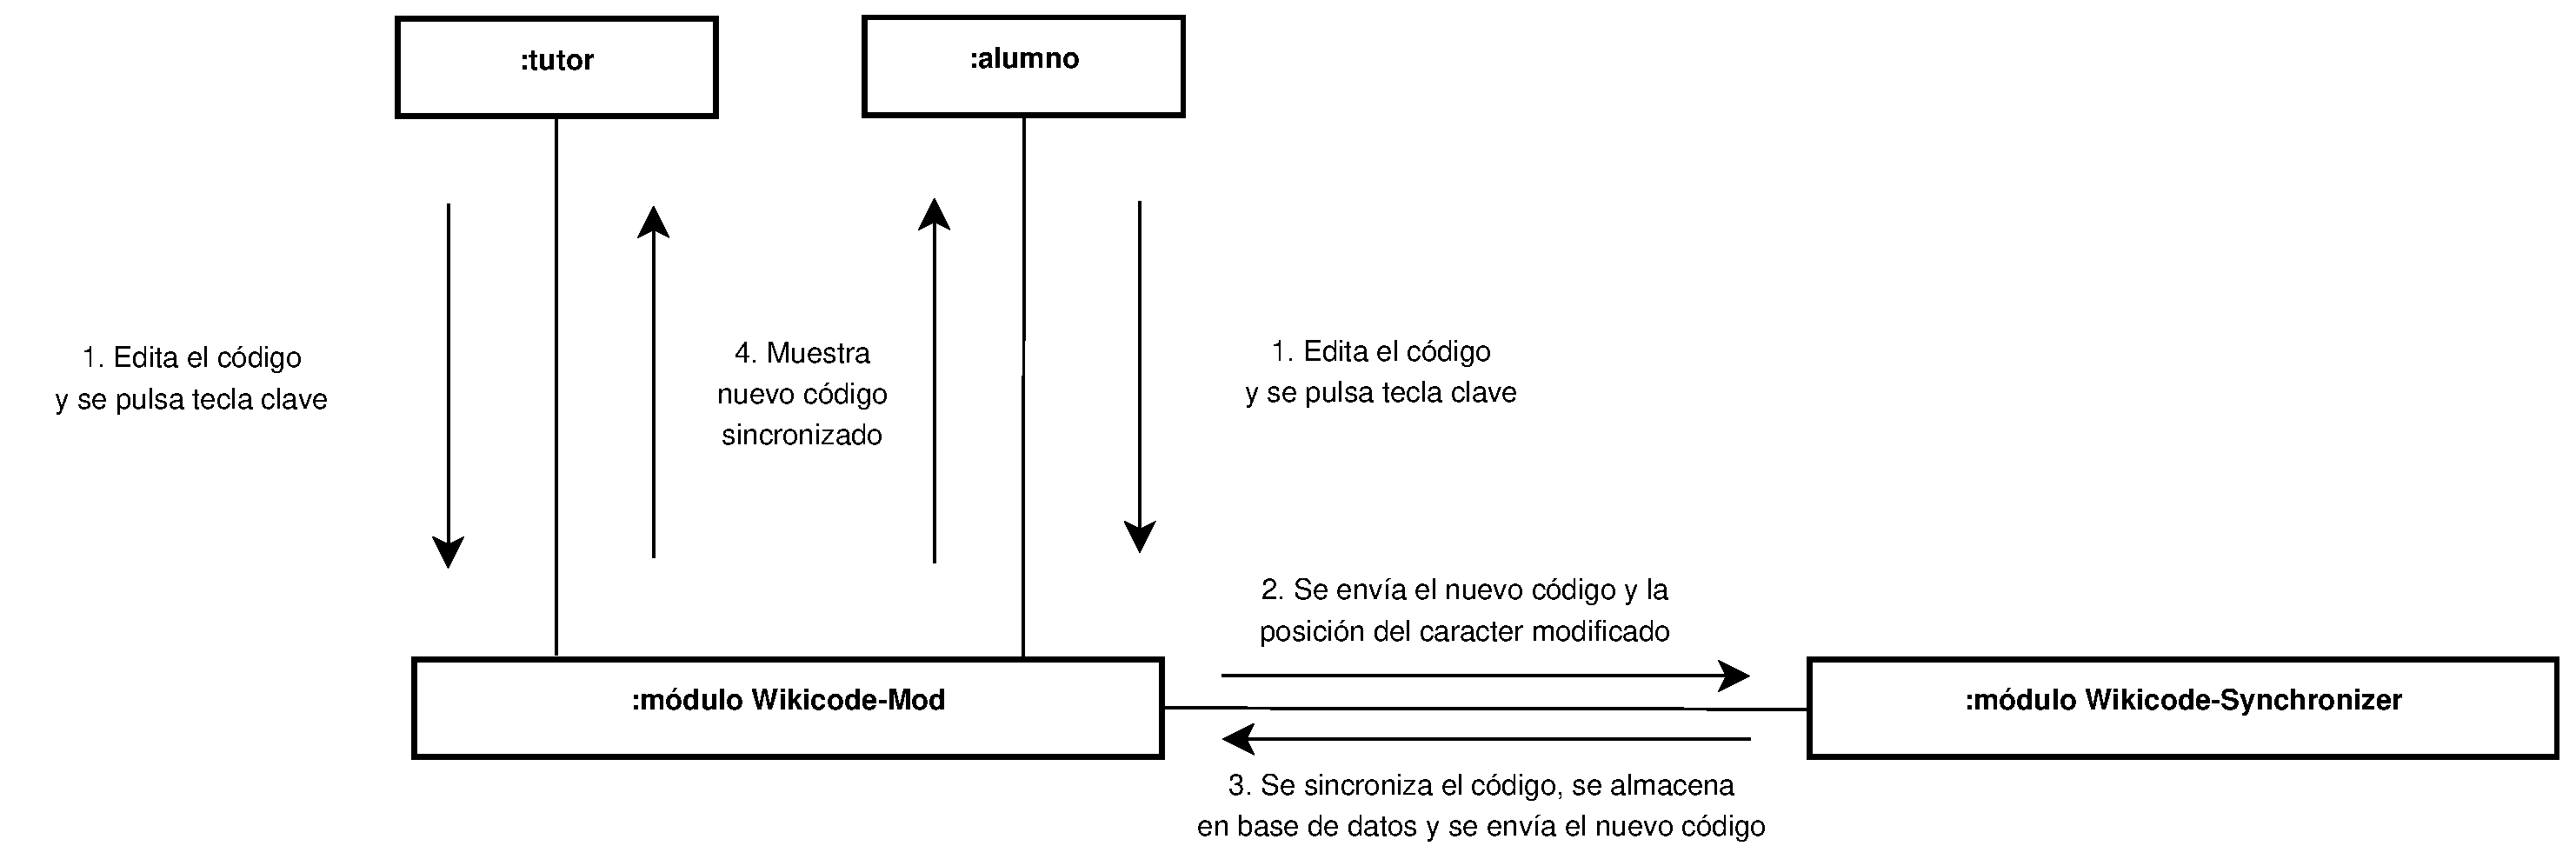
\includegraphics[width=\textwidth]{./img/c3-dia-col4.eps}
	\caption{Diagrama de colaboración Edición de código}
\end{figure}




































